% Created 2023-11-08 on 15:30
% Intended LaTeX compiler: pdflatex
\documentclass[12pt]{article}

%%%% settings when exporting code %%%% 

\usepackage{listings}
\lstdefinestyle{code-small}{
backgroundcolor=\color{white}, % background color for the code block
basicstyle=\ttfamily\small, % font used to display the code
commentstyle=\color[rgb]{0.5,0,0.5}, % color used to display comments in the code
keywordstyle=\color{black}, % color used to highlight certain words in the code
numberstyle=\ttfamily\tiny\color{gray}, % color used to display the line numbers
rulecolor=\color{black}, % color of the frame
stringstyle=\color[rgb]{0,.5,0},  % color used to display strings in the code
breakatwhitespace=false, % sets if automatic breaks should only happen at whitespace
breaklines=true, % sets automatic line breaking
columns=fullflexible,
frame=single, % adds a frame around the code (non,leftline,topline,bottomline,lines,single,shadowbox)
keepspaces=true, % % keeps spaces in text, useful for keeping indentation of code
literate={~}{$\sim$}{1}, % symbol properly display via latex
numbers=none, % where to put the line-numbers; possible values are (none, left, right)
numbersep=10pt, % how far the line-numbers are from the code
showspaces=false,
showstringspaces=false,
stepnumber=1, % the step between two line-numbers. If it's 1, each line will be numbered
tabsize=1,
xleftmargin=0cm,
emph={anova,apply,class,coef,colnames,colNames,colSums,dim,dcast,for,ggplot,head,if,ifelse,is.na,lapply,list.files,library,logLik,melt,plot,require,rowSums,sapply,setcolorder,setkey,str,summary,tapply},
aboveskip = \medskipamount, % define the space above displayed listings.
belowskip = \medskipamount, % define the space above displayed listings.
lineskip = 0pt} % specifies additional space between lines in listings
\lstset{style=code-small}
%%%% packages %%%%%

\usepackage[utf8]{inputenc}
\usepackage[T1]{fontenc}
\usepackage{lmodern}
\usepackage{textcomp}
\usepackage{color}
\usepackage{graphicx}
\usepackage{grffile}
\usepackage{wrapfig}
\usepackage{rotating}
\usepackage{longtable}
\usepackage{multirow}
\usepackage{multicol}
\usepackage{changes}
\usepackage{pdflscape}
\usepackage{geometry}
\usepackage[normalem]{ulem}
\usepackage{amssymb}
\usepackage{amsmath}
\usepackage{amsfonts}
\usepackage{dsfont}
\usepackage{array}
\usepackage{ifthen}
\usepackage{hyperref}
\usepackage{natbib}
\RequirePackage{setspace} % to modify the space between lines - incompatible with footnote in beamer
\renewcommand{\baselinestretch}{1.1}
\geometry{a4paper, left=10mm, right=10mm, top=10mm}
\usepackage{titlesec}
\usepackage{etoolbox}

\makeatletter
\patchcmd{\ttlh@hang}{\parindent\z@}{\parindent\z@\leavevmode}{}{}
\patchcmd{\ttlh@hang}{\noindent}{}{}{}
\makeatother
\RequirePackage{colortbl} % arrayrulecolor to mix colors
\definecolor{myorange}{rgb}{1,0.2,0}
\definecolor{mypurple}{rgb}{0.7,0,8}
\definecolor{mycyan}{rgb}{0,0.6,0.6}
\newcommand{\lightblue}{blue!50!white}
\newcommand{\darkblue}{blue!80!black}
\newcommand{\darkgreen}{green!50!black}
\newcommand{\darkred}{red!50!black}
\definecolor{gray}{gray}{0.5}
\hypersetup{
citecolor=[rgb]{0,0.5,0},
urlcolor=[rgb]{0,0,0.5},
linkcolor=[rgb]{0,0,0.5},
}
\newenvironment{note}{\small \color{gray}\fontfamily{lmtt}\selectfont}{\par}
\newenvironment{activity}{\color{orange}\fontfamily{qzc}\selectfont}{\par}
\RequirePackage{pifont}
\RequirePackage{relsize}
\newcommand{\Cross}{{\raisebox{-0.5ex}%
{\relsize{1.5}\ding{56}}}\hspace{1pt} }
\newcommand{\Valid}{{\raisebox{-0.5ex}%
{\relsize{1.5}\ding{52}}}\hspace{1pt} }
\newcommand{\CrossR}{ \textcolor{red}{\Cross} }
\newcommand{\ValidV}{ \textcolor{green}{\Valid} }
\usepackage{stackengine}
\usepackage{scalerel}
\newcommand\Warning[1][3ex]{%
\renewcommand\stacktype{L}%
\scaleto{\stackon[1.3pt]{\color{red}$\triangle$}{\tiny\bfseries !}}{#1}%
\xspace
}
\RequirePackage{fancyvrb}
\DefineVerbatimEnvironment{verbatim}{Verbatim}{fontsize=\small,formatcom = {\color[rgb]{0.5,0,0}}}
\definecolor{grayR}{HTML}{8A8990}
\definecolor{grayL}{HTML}{C4C7C9}
\definecolor{blueM}{HTML}{1F63B5}
\newcommand{\Rlogo}[1][0.07]{
\begin{tikzpicture}[scale=#1]
\shade [right color=grayR,left color=grayL,shading angle=60]
(-3.55,0.3) .. controls (-3.55,1.75)
and (-1.9,2.7) .. (0,2.7) .. controls (2.05,2.7)
and (3.5,1.6) .. (3.5,0.3) .. controls (3.5,-1.2)
and (1.55,-2) .. (0,-2) .. controls (-2.3,-2)
and (-3.55,-0.75) .. cycle;

\fill[white]
(-2.15,0.2) .. controls (-2.15,1.2)
and (-0.7,1.8) .. (0.5,1.8) .. controls (2.2,1.8)
and (3.1,1.2) .. (3.1,0.2) .. controls (3.1,-0.75)
and (2.4,-1.45) .. (0.5,-1.45) .. controls (-1.1,-1.45)
and (-2.15,-0.7) .. cycle;

\fill[blueM]
(1.75,1.25) -- (-0.65,1.25) -- (-0.65,-2.75) -- (0.55,-2.75) -- (0.55,-1.15) --
(0.95,-1.15)  .. controls (1.15,-1.15)
and (1.5,-1.9) .. (1.9,-2.75) -- (3.25,-2.75)  .. controls (2.2,-1)
and (2.5,-1.2) .. (1.8,-0.95) .. controls (2.6,-0.9)
and (2.85,-0.35) .. (2.85,0.2) .. controls (2.85,0.7)
and (2.5,1.2) .. cycle;

\fill[white]  (1.4,0.4) -- (0.55,0.4) -- (0.55,-0.3) -- (1.4,-0.3).. controls (1.75,-0.3)
and (1.75,0.4) .. cycle;

\end{tikzpicture}
}
\RequirePackage{epstopdf} % to be able to convert .eps to .pdf image files
\RequirePackage{capt-of} %
\RequirePackage{caption} % newlines in graphics
\RequirePackage{tikz-cd} % graph
\RequirePackage{booktabs} % for nice lines in table (e.g. toprule, bottomrule, midrule, cmidrule)
\RequirePackage{amsmath}
\RequirePackage{algorithm}
\RequirePackage[noend]{algpseudocode}
\RequirePackage{dsfont}
\RequirePackage{amsmath,stmaryrd,graphicx}
\RequirePackage{prodint} % product integral symbol (\PRODI)
\usepackage{ifthen}
\usepackage{xifthen}
\usepackage{xargs}
\usepackage{xspace}
\newcommand\defOperator[7]{%
\ifthenelse{\isempty{#2}}{
\ifthenelse{\isempty{#1}}{#7{#3}#4}{#7{#3}#4 \left#5 #1 \right#6}
}{
\ifthenelse{\isempty{#1}}{#7{#3}#4_{#2}}{#7{#3}#4_{#1}\left#5 #2 \right#6}
}
}
\newcommand\defUOperator[5]{%
\ifthenelse{\isempty{#1}}{
#5\left#3 #2 \right#4
}{
\ifthenelse{\isempty{#2}}{\underset{#1}{\operatornamewithlimits{#5}}}{
\underset{#1}{\operatornamewithlimits{#5}}\left#3 #2 \right#4}
}
}
\newcommand{\defBoldVar}[2]{
\ifthenelse{\equal{#2}{T}}{\boldsymbol{#1}}{\mathbf{#1}}
}
\newcommandx\Esp[2][1=,2=]{\defOperator{#1}{#2}{E}{}{\lbrack}{\rbrack}{\mathbb}}
\newcommandx\Prob[2][1=,2=]{\defOperator{#1}{#2}{P}{}{\lbrack}{\rbrack}{\mathbb}}
\newcommandx\Qrob[2][1=,2=]{\defOperator{#1}{#2}{Q}{}{\lbrack}{\rbrack}{\mathbb}}
\newcommandx\Var[2][1=,2=]{\defOperator{#1}{#2}{V}{ar}{\lbrack}{\rbrack}{\mathbb}}
\newcommandx\Cov[2][1=,2=]{\defOperator{#1}{#2}{C}{ov}{\lbrack}{\rbrack}{\mathbb}}
\newcommandx\Binom[2][1=,2=]{\defOperator{#1}{#2}{B}{}{(}{)}{\mathcal}}
\newcommandx\Gaus[2][1=,2=]{\defOperator{#1}{#2}{N}{}{(}{)}{\mathcal}}
\newcommandx\Wishart[2][1=,2=]{\defOperator{#1}{#2}{W}{ishart}{(}{)}{\mathcal}}
\newcommandx\Likelihood[2][1=,2=]{\defOperator{#1}{#2}{L}{}{(}{)}{\mathcal}}
\newcommandx\logLikelihood[2][1=,2=]{\defOperator{#1}{#2}{\ell}{}{(}{)}{}}
\newcommandx\Information[2][1=,2=]{\defOperator{#1}{#2}{I}{}{(}{)}{\mathcal}}
\newcommandx\Hessian[2][1=,2=]{\defOperator{#1}{#2}{H}{}{(}{)}{\mathcal}}
\newcommandx\Score[2][1=,2=]{\defOperator{#1}{#2}{S}{}{(}{)}{\mathcal}}
\newcommandx\Vois[2][1=,2=]{\defOperator{#1}{#2}{V}{}{(}{)}{\mathcal}}
\newcommandx\IF[2][1=,2=]{\defOperator{#1}{#2}{IF}{}{(}{)}{\mathcal}}
\newcommandx\Ind[1][1=]{\defOperator{}{#1}{1}{}{(}{)}{\mathds}}
\newcommandx\Max[2][1=,2=]{\defUOperator{#1}{#2}{(}{)}{min}}
\newcommandx\Min[2][1=,2=]{\defUOperator{#1}{#2}{(}{)}{max}}
\newcommandx\argMax[2][1=,2=]{\defUOperator{#1}{#2}{(}{)}{argmax}}
\newcommandx\argMin[2][1=,2=]{\defUOperator{#1}{#2}{(}{)}{argmin}}
\newcommandx\cvD[2][1=D,2=n \rightarrow \infty]{\xrightarrow[#2]{#1}}
\newcommandx\Hypothesis[2][1=,2=]{
\ifthenelse{\isempty{#1}}{
\mathcal{H}
}{
\ifthenelse{\isempty{#2}}{
\mathcal{H}_{#1}
}{
\mathcal{H}^{(#2)}_{#1}
}
}
}
\newcommandx\dpartial[4][1=,2=,3=,4=\partial]{
\ifthenelse{\isempty{#3}}{
\frac{#4 #1}{#4 #2}
}{
\left.\frac{#4 #1}{#4 #2}\right\rvert_{#3}
}
}
\newcommandx\dTpartial[3][1=,2=,3=]{\dpartial[#1][#2][#3][d]}
\newcommandx\ddpartial[3][1=,2=,3=]{
\ifthenelse{\isempty{#3}}{
\frac{\partial^{2} #1}{\partial #2^2}
}{
\frac{\partial^2 #1}{\partial #2\partial #3}
}
}
\newcommand\Real{\mathbb{R}}
\newcommand\Rational{\mathbb{Q}}
\newcommand\Natural{\mathbb{N}}
\newcommand\trans[1]{{#1}^\intercal}%\newcommand\trans[1]{{\vphantom{#1}}^\top{#1}}
\newcommand{\independent}{\mathrel{\text{\scalebox{1.5}{$\perp\mkern-10mu\perp$}}}}
\newcommand\half{\frac{1}{2}}
\newcommand\normMax[1]{\left|\left|#1\right|\right|_{max}}
\newcommand\normTwo[1]{\left|\left|#1\right|\right|_{2}}
\newcommand\Veta{\boldsymbol{\eta}}
\newcommand{\Model}{\mathcal{M}}
\newcommand{\ModelHat}{\widehat{\mathcal{M}}}
\newcommand{\param}{\Theta}
\newcommand{\paramHat}{\widehat{\param}}
\newcommand{\paramCon}{\widetilde{\param}}
\newcommand{\Vparam}{\boldsymbol{\param}}
\newcommand{\VparamT}{\Vparam_0}
\newcommand{\VparamHat}{\boldsymbol{\paramHat}}
\newcommand{\VparamCon}{\boldsymbol{\paramCon}}
\newcommand{\X}{X}
\newcommand{\x}{x}
\newcommand{\VX}{\boldsymbol{X}}
\newcommand{\Vx}{\boldsymbol{x}}
\newcommand{\Y}{Y}
\newcommand{\y}{y}
\newcommand{\VY}{\boldsymbol{Y}}
\newcommand{\Vy}{\boldsymbol{y}}
\newcommand{\Vvarepsilon}{\boldsymbol{\varepsilon}}
\author{Brice Ozenne}
\date{\today}
\title{Overview of the package LMMstar}
\hypersetup{
 colorlinks=true,
 pdfauthor={Brice Ozenne},
 pdftitle={Overview of the package LMMstar},
 pdfkeywords={},
 pdfsubject={},
 pdfcreator={Emacs 27.2 (Org mode 9.5.2)},
 pdflang={English}
 }
\begin{document}

\maketitle
This vignette describes the main functionalities of the \textbf{LMMstar}
package. This package implements specific types of linear mixed
models, mainly useful when having repeated observations over a
discrete variable: \(\VY=(Y_1,\ldots,Y_T)\) where \(T\) can be
for example be time (chronological ordering of the repetitions) or
brain region (arbitrary ordering of the repetitions). Denoting by
\(X\) the associated covariates and \(\boldsymbol{\varepsilon} =
(\varepsilon_1,\ldots,\varepsilon_T)\), the model can be written:
\[ \VY = X \beta + \boldsymbol{\varepsilon} \text{ where } \varepsilon \sim \Gaus(0,\Omega) \]
where \(\beta\) are the mean parameters and the residual
variance-covariance matrix, \(\Omega\), depends on a set of
variance-covariance parameters (say \(\gamma\)) distinct of
\(\beta\). Key assumptions are:
\begin{itemize}
\item we observe \(n\) independent replicates of
\(\mathcal{O}=(\VY,X)\), i.e. at the cluster level,
observations \(\left(\mathcal{O}_1,\ldots,\mathcal{O}_n\right)\) are
independent. The replicates should also be identically distributed
up to a categorical variable (called strata variable in the following).
\item the residual variance is independent of the mean value.
\end{itemize}
Additional assumptions are necessary in presence of missing values,
typically correct specification of the conditional mean to have
consistent estimates of the mean parameters. This case will sometimes
be examplified by considering that only last outcome may be missing:
the conditional mean \(\Esp[Y_T|Y_1,Y_2,\ldots,Y_{T-1}]\) is then
abreviated as \(\Esp[Y_T|Y_{T-1}]\). Note that we do not require the
residuals to be normally distributed to have valid estimates or
statistical inference in large samples.

\bigskip

To get start, one should load the \textbf{LMMstar} package in the \Rlogo session:
\lstset{language=r,label= ,caption= ,captionpos=b,numbers=none}
\begin{lstlisting}
library(LMMstar)
\end{lstlisting}

This package is under active development. Newer package versions may
include additional functionalities and fix previous bugs. The version
of the package that is being used for this overview is:
\lstset{language=r,label= ,caption= ,captionpos=b,numbers=none}
\begin{lstlisting}
utils::packageVersion("LMMstar")
\end{lstlisting}

\begin{verbatim}
[1] '1.0.0'
\end{verbatim}


\clearpage

The user interface of the \textbf{LMMstar} package is made of the following
functions:
\begin{itemize}
\item the function \texttt{lmm} is the main function of the package which fits
linear mixed models. The user can interact with \emph{lmm} objects using:
\begin{itemize}
\item \texttt{anova} to perform Wald tests, i.e. test linear combinations of
coefficients (\(\widehat{\beta}_1+\widehat{\beta}_2=0\) or
\(\widehat{\beta}_1=\widehat{\beta}_2=0\)). The output obtained
with different \texttt{lmm} can be combined using \texttt{rbind}.
\item \texttt{coef} to extract the estimated model parameters (\(\widehat{\beta}\) and possibly \(\widehat{\gamma}\)).
\item \texttt{confint} to extract the estimates with their confidence intervals.
\item \texttt{dummy.coef} to extract the estimated (marginal) mean for each combination of categorical covariate.
\item \texttt{estimate} to test non-linear combinations of coefficients (Wald test via a first order delta method, e.g. \(\widehat{\beta}_1/\widehat{\beta}_2=1\)).
\item \texttt{fitted} to output the fitted mean (\(X\widehat{\beta}\)) or the
conditional mean for observations with missing outcome
(e.g. \(X\widehat{\beta} +
      \widehat{\Esp}[\varepsilon_T|\varepsilon_{-T}]\)).
\item \texttt{iid} to extract the influence function of the estimated
parameters (\(\varphi\)), which satisfies \newline
\(\sqrt{n}(\widehat{\beta}-\beta) = \frac{1}{\sqrt{n}}
      \sum_{i=1}^n \varphi\left(\mathcal{O}_i\right) +o_p(1)\)
\item \texttt{levels} to extract the reference level for the mean structure.
(i.e. what \texttt{(Intercept)} refers to in presence of categorical.
covariates).
\item \texttt{logLik} to output the log-likelihood of the estimated model.
\item \texttt{model.tables} to extract the estimates, standard errors, p-value, and confidence intervals.
\item \texttt{plot} to obtain a diagnostic plots, partial residual plots, or a graphical display of the fitted values.
\item \texttt{predict} to compute the mean conditional on covariates and
possible outcome values.
\item \texttt{profile} to display the likelihood or profile likelihood of the model.
\item \texttt{resample} to use non-parametric bootstrap or permutation test for statistical inference.
\item \texttt{residuals} to extract the observed residuals of the fitted
model, possibly normalized
(\(\widehat{\Omega}^{-\frac{1}{2}}\widehat{\varepsilon}\)).
\item \texttt{sigma} to extract the modeled residual variance covariance matrix (\(\widehat{\Omega}\)).
\item \texttt{summary} to obtain a summary of the input, model fit, and estimated values.
\item \texttt{vcov} to extract the variance-covariance matrix of the mean
parameters (\(\widehat{\Sigma}_{\widehat{\beta}}\)).
\end{itemize}
\item the \texttt{mlmm} function to fit group-specific linear mixed models and
gather the estimated coefficients.
\item the \texttt{summarize} function to compute summary statistics, possibly
stratified on a categorical variable
\item the \texttt{summarizeNA} function to identify missing data patterns.
\item the \texttt{partialCor} function to compute partial correlation between two variables.
\item the \texttt{sampleRem} function to simulate longitudinal data.
\item the \texttt{LMMstar.options} function enables the user to display the
default values used in the \textbf{LMMstar} package. The function
can also change the default values to better match the user needs.
\end{itemize}


\clearpage

\section{Illustrative dataset}
\label{sec:org43fa78c}
To illustrate the functionalities of the package, we will use the
gastricbypass dataset. The long format can be imported using:
\lstset{language=r,label= ,caption= ,captionpos=b,numbers=none}
\begin{lstlisting}
data(gastricbypassL, package = "LMMstar")
head(gastricbypassL)
\end{lstlisting}

\begin{verbatim}
  id visit          time weight glucagonAUC
1  1     1 3monthsBefore  127.2     5032.50
2  2     1 3monthsBefore  165.2    12142.50
3  3     1 3monthsBefore  109.7    10321.35
4  4     1 3monthsBefore  146.2     6693.00
5  5     1 3monthsBefore  113.1     7090.50
6  6     1 3monthsBefore  158.8    10386.00
\end{verbatim}


See \texttt{?gastricbypassL} for a presentation of the dataset. We will
shorten the values of the time variable:
\lstset{language=r,label= ,caption= ,captionpos=b,numbers=none}
\begin{lstlisting}
gastricbypassL$time <- factor(gastricbypassL$time,
                              levels = c("3monthsBefore", "1weekBefore",
                                         "1weekAfter", "3monthsAfter" ),
                              labels = c("B3m","B1w","A1w","A3m"))
gastricbypassL$visit <- as.numeric(gastricbypassL$time) ## convert to numeric
gastricbypassL$baseline <- gastricbypassL$visit<=2
\end{lstlisting}
rescale the glucagon values
\lstset{language=r,label= ,caption= ,captionpos=b,numbers=none}
\begin{lstlisting}
gastricbypassL$glucagon <- as.double(scale(gastricbypassL$glucagonAUC))+5
\end{lstlisting}

and add a group variable:
\lstset{language=r,label= ,caption= ,captionpos=b,numbers=none}
\begin{lstlisting}
gastricbypassL$group <- as.numeric(gastricbypassL$id)%%2
\end{lstlisting}

The corresponding wide format is
\lstset{language=r,label= ,caption= ,captionpos=b,numbers=none}
\begin{lstlisting}
data(gastricbypassW, package = "LMMstar")
head(gastricbypassW)
\end{lstlisting}

\begin{verbatim}
  id weight1 weight2 weight3 weight4 glucagonAUC1 glucagonAUC2 glucagonAUC3 glucagonAUC4
1  1   127.2   120.7   115.5   108.1      5032.50       4942.5      20421.0      9249.45
2  2   165.2   153.4   149.2   132.0     12142.50      14083.5      10945.5      7612.50
3  3   109.7   101.6    97.7    87.1     10321.35       6202.5      20121.0     17704.50
4  4   146.2   142.4   136.7   123.0      6693.00       6631.5      13090.5      4551.00
5  5   113.1   105.6    99.9    87.7      7090.50           NA      19155.0     12345.00
6  6   158.8   143.6   134.6   108.7     10386.00       7609.5      11778.0      8014.80
\end{verbatim}


for which we can also add the group variable:
\lstset{language=r,label= ,caption= ,captionpos=b,numbers=none}
\begin{lstlisting}
gastricbypassW$group <- as.numeric(gastricbypassW$id)%%2
\end{lstlisting}

Finally we will remove observation with missing glucagon values:
\lstset{language=r,label= ,caption= ,captionpos=b,numbers=none}
\begin{lstlisting}
dfL <- gastricbypassL[!is.na(gastricbypassL$glucagonAUC),]
\end{lstlisting}

\clearpage

\section{Descriptive statistics}
\label{sec:org1565a4e}
\subsection{Summary statistics}
\label{sec:orgfa1411a}

Mean, standard deviation, and other summary statistic can be computed
with respect to a categorical variable (typically time) using the
\texttt{summarize} function:
\lstset{language=r,label= ,caption= ,captionpos=b,numbers=none}
\begin{lstlisting}
sss <- summarize(weight+glucagon ~ time, data = gastricbypassL, na.rm = TRUE)
print(sss, digits = 3)
\end{lstlisting}

\begin{verbatim}
   outcome time observed missing   mean     sd    min     q1 median     q3    max
1   weight  B3m       20       0 128.97 20.269 100.90 115.30 123.10 139.82 173.00
2           B1w       20       0 121.24 18.910  95.70 107.78 114.50 134.53 162.20
3           A1w       20       0 115.70 18.275  89.90 102.22 110.60 128.38 155.00
4           A3m       20       0 102.36 17.054  78.80  90.40  98.50 108.25 148.00
5 glucagon  B3m       20       0   4.51  0.641   3.61   4.06   4.33   4.93   6.03
6           B1w       19       1   4.39  0.558   3.58   4.05   4.23   4.55   5.95
7           A1w       19       1   6.06  1.044   4.52   5.30   5.94   6.62   8.27
8           A3m       20       0   5.06  0.760   3.95   4.52   5.03   5.27   7.12
\end{verbatim}


Correlation matrices are also ouput when a cluster and ordering
variable have been specified (here respectively \texttt{id} and \texttt{time}):
\lstset{language=r,label= ,caption= ,captionpos=b,numbers=none}
\begin{lstlisting}
sss <- summarize(weight ~ time|id, data = gastricbypassL, na.rm = TRUE)
print(sss, digits = 3)
\end{lstlisting}

\begin{verbatim}
  time observed missing mean   sd   min    q1 median  q3 max
1  B3m       20       0  129 20.3 100.9 115.3  123.1 140 173
2  B1w       20       0  121 18.9  95.7 107.8  114.5 135 162
3  A1w       20       0  116 18.3  89.9 102.2  110.6 128 155
4  A3m       20       0  102 17.1  78.8  90.4   98.5 108 148

 Pearson's correlation: 
      B3m   B1w   A1w   A3m
B3m 1.000 0.990 0.986 0.946
B1w 0.990 1.000 0.997 0.959
A1w 0.986 0.997 1.000 0.966
A3m 0.946 0.959 0.966 1.000
\end{verbatim}

Alternatively, the \texttt{partialCor} function can be used to compute
correlation from the wide format, e.g.:
\lstset{language=r,label= ,caption= ,captionpos=b,numbers=none}
\begin{lstlisting}
partialCor(weight1 + weight4 ~ 1, data = gastricbypassW)
\end{lstlisting}

\begin{verbatim}
                     estimate    se   df lower upper  p.value
rho(weight1,weight4)    0.946 0.105 31.1 0.867 0.978 8.46e-09
\end{verbatim}


\clearpage

Partial correlations can be also computed, e.g.:
\lstset{language=r,label= ,caption= ,captionpos=b,numbers=none}
\begin{lstlisting}
partialCor(list(weight1 ~ glucagonAUC1, weight4 ~ glucagonAUC4),
           data = gastricbypassW)
\end{lstlisting}

\begin{verbatim}
                     estimate    se   df lower upper  p.value
rho(weight1,weight4)    0.946 0.109 19.6 0.859  0.98 3.62e-07
\end{verbatim}


The \texttt{partialCor} function can also be used to obtain group-specific
correlations:
\lstset{language=r,label= ,caption= ,captionpos=b,numbers=none}
\begin{lstlisting}
partialCor(weight + glucagonAUC ~ 1, by = "group", data = gastricbypassL)
\end{lstlisting}

\begin{verbatim}
                           estimate    se   df  lower   upper p.value
0: rho(weight,glucagonAUC)   -0.281 0.148 21.1 -0.552  0.0442  0.0858
1: rho(weight,glucagonAUC)   -0.336 0.144 22.2 -0.594 -0.0156  0.0410
\end{verbatim}


A p-value for the difference can be obtained specifying the argument
\texttt{effects}:
\lstset{language=r,label= ,caption= ,captionpos=b,numbers=none}
\begin{lstlisting}
partialCor(weight + glucagonAUC ~ 1, by = "group", effects = "Dunnett",
           data = gastricbypassL)
\end{lstlisting}

\begin{verbatim}
                                                      estimate se df lower upper p.value
1:rho(weight,glucagonAUC) - 0:rho(weight,glucagonAUC)   -0.055 NA NA    NA    NA   0.789
\end{verbatim}

\subsection{Missing data patterns}
\label{sec:org1b0c823}

The \texttt{summarizeNA} identify the possible combinations of
observed/missing data:
\lstset{language=r,label= ,caption= ,captionpos=b,numbers=none}
\begin{lstlisting}
mp <- summarizeNA(gastricbypassL)
mp
\end{lstlisting}

\begin{verbatim}
frequency missing.pattern n.missing id visit time weight glucagonAUC baseline glucagon group
       78        00000000         0  0     0    0      0           0        0        0     0
        2        00001010         2  0     0    0      0           1        0        1     0
\end{verbatim}


A graphical representation can be obtained using \texttt{plot}:
\lstset{language=r,label= ,caption= ,captionpos=b,numbers=none}
\begin{lstlisting}
plot(mp)
\end{lstlisting}

\begin{center}
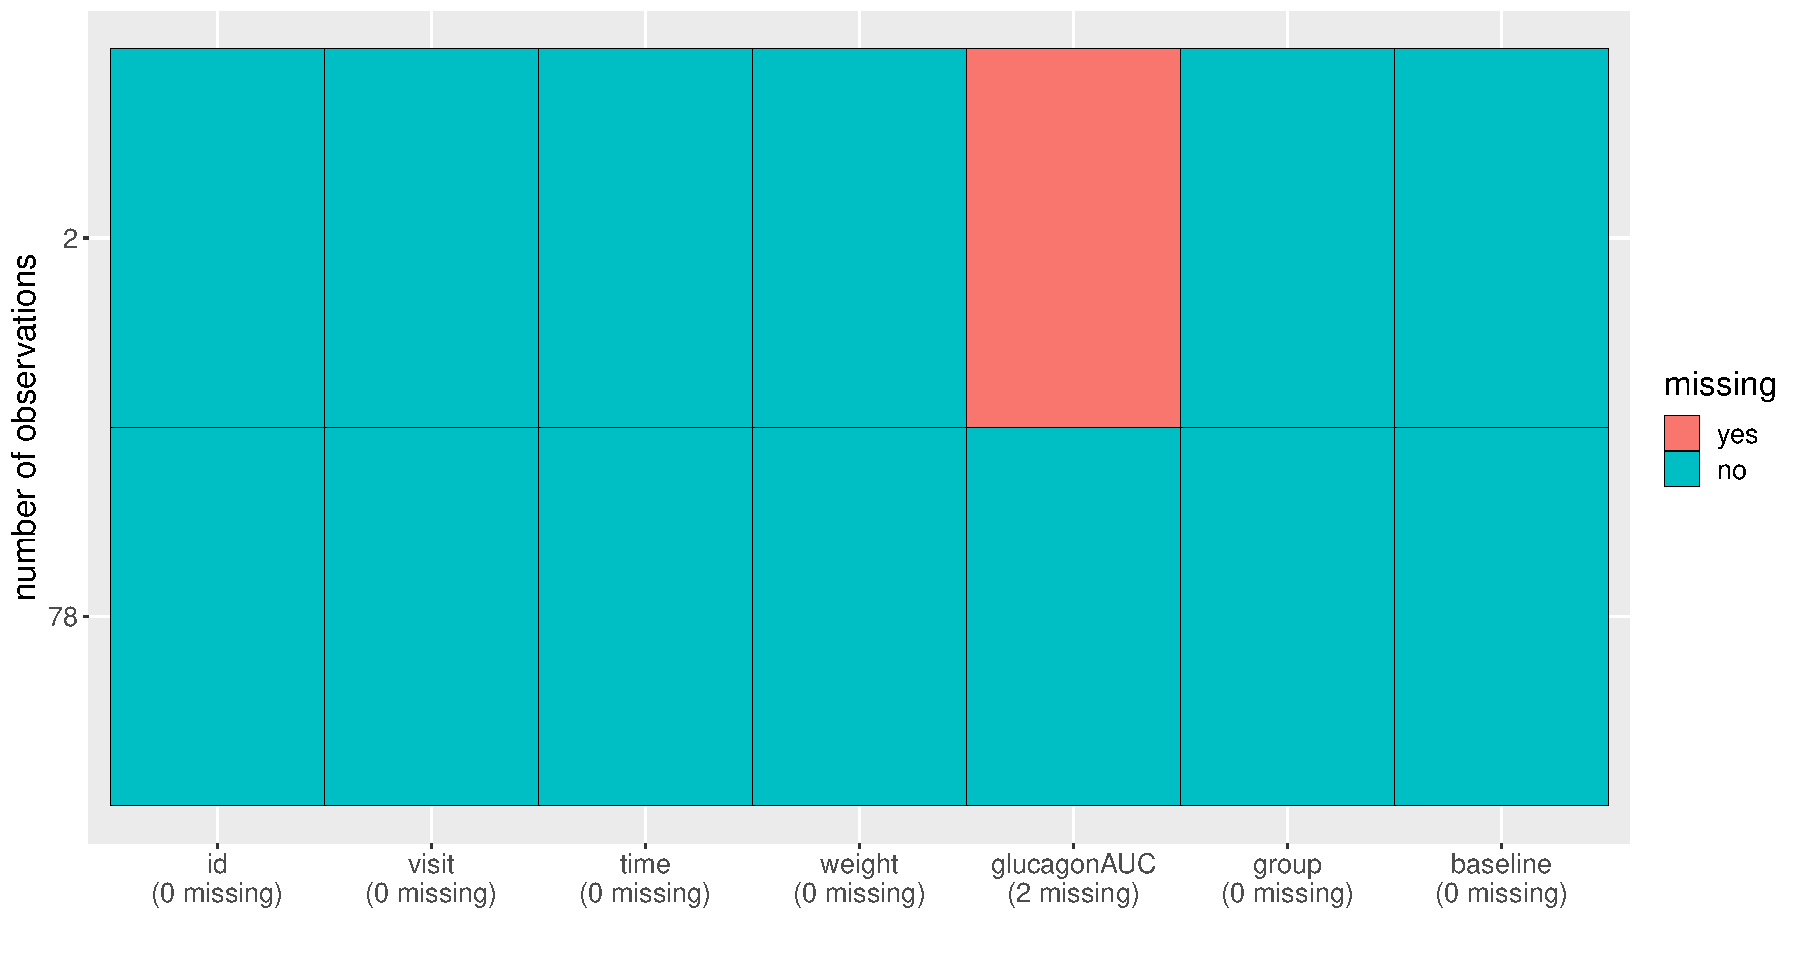
\includegraphics[trim={0 0 0 0},width=1\textwidth]{./figures/summarizeNA.pdf}
\end{center}



\clearpage

\section{Linear mixed model (LMM)}
\label{sec:org85ec94e}
\subsection{Classical covariance patterns}
\label{sec:org803e9f6}

Several build-in covariance patterns can be used when specifying the
linear model. The most basic ones are the \textbf{identity} structure:
\lstset{language=r,label= ,caption= ,captionpos=b,numbers=none}
\begin{lstlisting}
eId.lmm <- lmm(weight ~ time + glucagon, repetition = ~time|id, 
               structure = "ID", data = dfL)
eId.lmm
cat(" modeled residual variance-covariance: \n");sigma(eId.lmm)
\end{lstlisting}

\begin{verbatim}
		Linear regression 

 outcome/cluster/time: weight/id/time 
 data                : 78 observations from 20 clusters 
 parameter           : 5 mean ((Intercept) timeB1w timeA1w timeA3m glucagon) 
                       1 variance (sigma) 
 log-restr.likelihood: -323.086426918519 
 convergence         : TRUE (0 iterations)
 modeled residual variance-covariance: 
         B3m      B1w      A1w      A3m
B3m 330.0427   0.0000   0.0000   0.0000
B1w   0.0000 330.0427   0.0000   0.0000
A1w   0.0000   0.0000 330.0427   0.0000
A3m   0.0000   0.0000   0.0000 330.0427
\end{verbatim}

and the \textbf{independence} structure:
\lstset{language=r,label= ,caption= ,captionpos=b,numbers=none}
\begin{lstlisting}
eInd.lmm <- lmm(weight ~ time + glucagon, repetition = ~time|id, 
               structure = "IND", data = dfL)
eInd.lmm
cat(" modeled residual variance-covariance: \n");sigma(eInd.lmm)
\end{lstlisting}

\begin{verbatim}
		Linear regression with heterogeneous residual variance 

 outcome/cluster/time: weight/id/time 
 data                : 78 observations from 20 clusters 
 parameter           : 5 mean ((Intercept) timeB1w timeA1w timeA3m glucagon) 
                       4 variance (sigma k.B1w k.A1w k.A3m) 
 log-restr.likelihood: -321.457830361849 
 convergence         : TRUE (8 iterations)
 modeled residual variance-covariance: 
         B3m      B1w      A1w      A3m
B3m 442.6475   0.0000   0.0000   0.0000
B1w   0.0000 418.9934   0.0000   0.0000
A1w   0.0000   0.0000 222.8463   0.0000
A3m   0.0000   0.0000   0.0000 237.2049
\end{verbatim}

\clearpage

The most common linear mixed model uses a \textbf{compound symmetry} structure:
\lstset{language=r,label= ,caption= ,captionpos=b,numbers=none}
\begin{lstlisting}
eCS.lmm <- lmm(weight ~ time + glucagon, repetition = ~time|id,
               structure = "CS", data = dfL)
eCS.lmm
cat(" modeled residual variance-covariance: \n");sigma(eCS.lmm)
\end{lstlisting}

\begin{verbatim}
		Linear Mixed Model with a compound symmetry covariance matrix 

 outcome/cluster/time: weight/id/time 
 data                : 78 observations from 20 clusters 
 parameter           : 5 mean ((Intercept) timeB1w timeA1w timeA3m glucagon) 
                       1 variance (sigma) 
                       1 correlation (rho) 
 log-restr.likelihood: -243.600523870252 
 convergence         : TRUE (9 iterations)
 modeled residual variance-covariance: 
         B3m      B1w      A1w      A3m
B3m 355.3062 344.6236 344.6236 344.6236
B1w 344.6236 355.3062 344.6236 344.6236
A1w 344.6236 344.6236 355.3062 344.6236
A3m 344.6236 344.6236 344.6236 355.3062
\end{verbatim}

\noindent A more flexible model can be obtained with a \textbf{toeplitz} covariance matrix:
\lstset{language=r,label= ,caption= ,captionpos=b,numbers=none}
\begin{lstlisting}
eTOE.lmm <- lmm(weight ~ time*group, repetition = ~time|id,
                structure = "TOEPLITZ", data = dfL)
eTOE.lmm
cat(" modeled residual correlation: \n");cov2cor(sigma(eTOE.lmm))
\end{lstlisting}

\begin{verbatim}

 outcome/cluster/time: weight/id/time 
 data                : 78 observations from 20 clusters 
 parameter           : 8 mean ((Intercept) timeB1w timeA1w timeA3m group timeB1w:group timeA1w:group timeA3m:group) 
                       4 variance (sigma k.B1w k.A1w k.A3m) 
                       3 correlation (rho(1) rho(2) rho(3)) 
 log-restr.likelihood: -221.152940926053 
 convergence         : TRUE (21 iterations)
 modeled residual correlation: 
          B3m       B1w       A1w       A3m
B3m 1.0000000 0.9854133 0.9676223 0.9489216
B1w 0.9854133 1.0000000 0.9854133 0.9676223
A1w 0.9676223 0.9854133 1.0000000 0.9854133
A3m 0.9489216 0.9676223 0.9854133 1.0000000
\end{verbatim}

\clearpage

\noindent And an even more flexible model can be obtained with an
\textbf{unstructured} covariance matrix:

\lstset{language=r,label= ,caption= ,captionpos=b,numbers=none}
\begin{lstlisting}
eUN.lmm <- lmm(weight ~ time + glucagon, repetition = ~time|id,
               structure = "UN", data = dfL)
eUN.lmm
cat(" modeled residual variance-covariance: \n");sigma(eUN.lmm)
\end{lstlisting}

\begin{verbatim}
		Linear Mixed Model with an unstructured covariance matrix 

 outcome/cluster/time: weight/id/time 
 data                : 78 observations from 20 clusters 
 parameter           : 5 mean ((Intercept) timeB1w timeA1w timeA3m glucagon) 
                       4 variance (sigma k.B1w k.A1w k.A3m) 
                       6 correlation (rho(B3m,B1w) rho(B3m,A1w) rho(B3m,A3m) rho(B1w,A1w) rho(B1w,A3m) rho(A1w,A3m)) 
 log-restr.likelihood: -216.318937004306 
 convergence         : TRUE (22 iterations)
 modeled residual variance-covariance: 
         B3m      B1w      A1w      A3m
B3m 411.3114 381.9734 352.6400 318.8573
B1w 381.9734 362.7326 335.4649 304.6314
A1w 352.6400 335.4649 311.6921 285.8077
A3m 318.8573 304.6314 285.8077 280.9323
\end{verbatim}

\noindent Stratification of the covariance structure on a categorical
variable is also possible:
\begin{itemize}
\item e.g. to get a \textbf{stratified compound symmetry}
\end{itemize}
\lstset{language=r,label= ,caption= ,captionpos=b,numbers=none}
\begin{lstlisting}
eSCS.lmm <- lmm(weight ~ time*group,
                repetition = ~time|id, structure = CS(group~1),
                data = dfL)
eSCS.lmm
\end{lstlisting}

\begin{verbatim}
	       Linear Mixed Model with a stratified compound symmetry covariance matrix 

outcome/cluster/time: weight/id/time 
data                : 78 observations from 20 clusters 
parameter           : 8 mean ((Intercept) timeB1w timeA1w timeA3m group timeB1w:group timeA1w:group timeA3m:group) 
                      2 variance (sigma:0 sigma:1) 
                      2 correlation (rho:0 rho:1) 
log-restr.likelihood: -229.203435252784 
convergence         : TRUE (6 iterations)
\end{verbatim}


\clearpage

\begin{itemize}
\item e.g. \textbf{stratified unstructured} covariance matrix:
\end{itemize}
\lstset{language=r,label= ,caption= ,captionpos=b,numbers=none}
\begin{lstlisting}
eSUN.lmm <- lmm(weight ~ time*group + glucagon,
                repetition = ~time|id, structure = UN(~group),
                data = dfL)
eSUN.lmm
\end{lstlisting}
\begin{verbatim}
	       Linear Mixed Model with a stratified unstructured covariance matrix 

outcome/cluster/time: weight/id/time 
data                : 78 observations from 20 clusters 
parameter           : 9 mean ((Intercept) timeB1w timeA1w timeA3m group glucagon timeB1w:group timeA1w:group timeA3m:group) 
                      8 variance (sigma:0 sigma:1 k.B1w:0 k.A1w:0 k.A3m:0 k.B1w:1 k.A1w:1 k.A3m:1) 
                      12 correlation (rho(B3m,B1w):0 rho(B3m,A1w):0 rho(B3m,A3m):0 rho(B1w,A1w):0 rho(B1w,A3m):0 rho(A1w,A3m):0 rho(B3m,B1w):1 rho(B3m,A1w):1 rho(B3m,A3m):1 rho(B1w,A1w):1 rho(B1w,A3m):1 rho(A1w,A3m):1) 
log-restr.likelihood: -197.171312062212 
convergence         : TRUE (50 iterations)
\end{verbatim}



with modeled residual variance-covariance:

\bigskip

\begin{minipage}{0.47\linewidth}
\lstset{language=r,label= ,caption= ,captionpos=b,numbers=none}
\begin{lstlisting}
sigma(eSCS.lmm)
\end{lstlisting}

\begin{verbatim}
$`1:1`
         B3m      B1w      A1w      A3m
B3m 348.0783 334.7404 334.7404 334.7404
B1w 334.7404 348.0783 334.7404 334.7404
A1w 334.7404 334.7404 348.0783 334.7404
A3m 334.7404 334.7404 334.7404 348.0783

$`3:3`
         B3m      B1w      A1w      A3m
B3m 345.5863 340.1538 340.1538 340.1538
B1w 340.1538 345.5863 340.1538 340.1538
A1w 340.1538 340.1538 345.5863 340.1538
A3m 340.1538 340.1538 340.1538 345.5863
\end{verbatim}
\end{minipage}
\begin{minipage}{0.47\linewidth}
\lstset{language=r,label= ,caption= ,captionpos=b,numbers=none}
\begin{lstlisting}
sigma(eSUN.lmm)
\end{lstlisting}

\begin{verbatim}
$`1:1`
         B3m      B1w      A1w      A3m
B3m 417.3374 382.8829 362.5674 301.7430
B1w 382.8829 364.4515 346.4039 292.7507
A1w 362.5674 346.4039 331.1789 282.9301
A3m 301.7430 292.7507 282.9301 253.3324

$`2:2`
         B3m      B1w      A1w      A3m
B3m 383.8877 363.6405 336.5771 350.0416
B1w 363.6405 347.9898 321.5908 331.5182
A1w 336.5771 321.5908 297.5329 308.1345
A3m 350.0416 331.5182 308.1345 334.8267
\end{verbatim}
\end{minipage}

\clearpage

\noindent Finally the some covariance patterns like the compound
symmetry structure may depend on covariates:
\begin{itemize}
\item e.g. to obtain a \textbf{block compound symmetry} structure\footnote{similar to
nested random effects}:
\end{itemize}
\lstset{language=r,label= ,caption= ,captionpos=b,numbers=none}
\begin{lstlisting}
eBCS.lmm <- lmm(weight ~ time*group,repetition = ~time|id,
                structure = CS(~baseline, type = "homogeneous"), data = dfL)
eBCS.lmm
cat(" modeled residual variance-covariance: \n");sigma(eBCS.lmm)
\end{lstlisting}

\begin{verbatim}
		Linear Mixed Model with a block compound symmetry covariance matrix 

 outcome/cluster/time: weight/id/time 
 data                : 78 observations from 20 clusters 
 parameter           : 8 mean ((Intercept) timeB1w timeA1w timeA3m group timeB1w:group timeA1w:group timeA3m:group) 
                       1 variance (sigma) 
                       2 correlation (rho(baseline) rho(id)) 
 log-restr.likelihood: -230.532819632968 
 convergence         : TRUE (6 iterations)
 modeled residual variance-covariance: 
         B3m      B1w      A1w      A3m
B3m 346.7441 339.3256 336.1825 336.1825
B1w 339.3256 346.7441 336.1825 336.1825
A1w 336.1825 336.1825 346.7441 339.3256
A3m 336.1825 336.1825 339.3256 346.7441
\end{verbatim}

\begin{itemize}
\item e.g. to obtain a \textbf{block unstructured} covariance matrix:
\end{itemize}
\lstset{language=r,label= ,caption= ,captionpos=b,numbers=none}
\begin{lstlisting}
eBUN.lmm <- lmm(weight ~ time*group, repetition = ~time|id,
                structure = CS(~baseline, type = "heterogeneous"), data = dfL)
eBUN.lmm
cat(" modeled residual variance-covariance: \n");sigma(eBUN.lmm)
\end{lstlisting}

\begin{verbatim}
		Linear Mixed Model with a block unstructured covariance matrix 

 outcome/cluster/time: weight/id/time 
 data                : 78 observations from 20 clusters 
 parameter           : 8 mean ((Intercept) timeB1w timeA1w timeA3m group timeB1w:group timeA1w:group timeA3m:group) 
                       2 variance (sigma k.TRUE) 
                       3 correlation (rho(FALSE) rho(FALSE,TRUE) rho(TRUE)) 
 log-restr.likelihood: -227.461008305704 
 convergence         : TRUE (6 iterations)
 modeled residual variance-covariance: 
         B3m      B1w      A1w      A3m
B3m 378.0328 372.8100 336.3064 336.3064
B1w 372.8100 378.0328 336.3064 336.3064
A1w 336.3064 336.3064 315.6358 306.0647
A3m 336.3064 336.3064 306.0647 315.6358
\end{verbatim}

\clearpage

\subsection{User-specific covariance patterns}
\label{sec:org7283dac}

It is possible input user-specific covariance patterns under the
following model for the residuals: \[\Omega =
\trans{\boldsymbol{\sigma}} R \boldsymbol{\sigma}\] where:
\begin{itemize}
\item \(\boldsymbol{\sigma}=f(\boldsymbol{\theta}_{\sigma},Z_{\sigma})\)
is a vector of residual standard errors depending on a vector of
parameters \(\boldsymbol{\theta}_{\sigma}\) and possible covariates
via the design matrix \(Z_{\sigma}\).
\item \(R=g(\boldsymbol{\theta}_{R},Z_R)\) is a matrix of residual
correlations depending on a vector of parameters
\(\boldsymbol{\theta}_{R}\) and possible covariates via the design
matrix \(Z_R\).
\end{itemize}

\bigskip

To be more concrete, consider the following correlation matrix
\lstset{language=r,label= ,caption= ,captionpos=b,numbers=none}
\begin{lstlisting}
rho.2block <- function(p,n.time,X){
  rho <- matrix(1, nrow = n.time, ncol = n.time)
  rho[1,2] <- rho[2,1] <- rho[4,5] <- rho[5,4] <- p["rho1"]
  rho[1,3] <- rho[3,1] <- rho[4,6] <- rho[6,4] <- p["rho2"]
  rho[2,3] <- rho[3,2] <- rho[5,6] <- rho[6,5] <- p["rho3"]
  rho[4:6,1:3] <- rho[1:3,4:6] <- p["rho4"]
  return(rho)
}
Rho <- rho.2block(p = c(rho1=0.25,rho2=0.5,rho3=0.4,rho4=0.1),
                  n.time = 6)
Rho
\end{lstlisting}

\begin{verbatim}
     [,1] [,2] [,3] [,4] [,5] [,6]
[1,] 1.00 0.25  0.5 0.10 0.10  0.1
[2,] 0.25 1.00  0.4 0.10 0.10  0.1
[3,] 0.50 0.40  1.0 0.10 0.10  0.1
[4,] 0.10 0.10  0.1 1.00 0.25  0.5
[5,] 0.10 0.10  0.1 0.25 1.00  0.4
[6,] 0.10 0.10  0.1 0.50 0.40  1.0
\end{verbatim}


and the corresponding dataset:
\lstset{language=r,label= ,caption= ,captionpos=b,numbers=none}
\begin{lstlisting}
set.seed(11)
n <- 1000
Y <- rmvnorm(n, mean = rep(0,6), sigma = Rho)
dfL2 <- reshape2::melt(cbind(id = 1:n, as.data.frame(Y)), id.vars = "id")
dfL2$time  <- dfL2$variable
dfL2 <- dfL2[order(dfL2$id),]
dfL2[1:8,]
\end{lstlisting}

\begin{verbatim}
     id variable      value time
1     1       V1 -0.9842079   V1
1001  1       V2 -0.3681245   V2
2001  1       V3 -1.6174652   V3
3001  1       V4 -1.4994103   V4
4001  1       V5  0.7493107   V5
5001  1       V6 -1.0719657   V6
2     2       V1  1.2402726   V1
1002  2       V2  0.6494215   V2
\end{verbatim}


To estimate the corresponding mixed model we first define a new
covariance structure:
\lstset{language=r,label= ,caption= ,captionpos=b,numbers=none}
\begin{lstlisting}
myStruct <- CUSTOM(~variable,
                   FCT.sigma = function(p,n.time,X){rep(p,n.time)}, ## function f
                   init.sigma = c("sigma"=1),
                   FCT.rho = rho.2block, ## function g
                   init.rho = c("rho1"=0.25,"rho2"=0.25,"rho3"=0.25,"rho4"=0.25))
\end{lstlisting}

and then call \texttt{lmm} with this structure structure:
\lstset{language=r,label= ,caption= ,captionpos=b,numbers=none}
\begin{lstlisting}
e.lmmCUSTOM <- lmm(value~time,
                   repetition=~time|id,
                   structure = myStruct,
                   data=dfL2,
                   df = FALSE) ## df = FALSE to save computation time
logLik(e.lmmCUSTOM)
\end{lstlisting}

\begin{verbatim}
[1] -7962.243
\end{verbatim}


The optimization procedure may be slow but should eventually reaches
an optimum. We can then output the estimated correlation matrix:
\lstset{language=r,label= ,caption= ,captionpos=b,numbers=none}
\begin{lstlisting}
cov2cor(sigma(e.lmmCUSTOM))
\end{lstlisting}

\begin{verbatim}
           V1         V2         V3         V4         V5         V6
V1 1.00000000 0.24898095 0.50058994 0.09053785 0.09053785 0.09053785
V2 0.24898095 1.00000000 0.36110943 0.09053785 0.09053785 0.09053785
V3 0.50058994 0.36110943 1.00000000 0.09053785 0.09053785 0.09053785
V4 0.09053785 0.09053785 0.09053785 1.00000000 0.24898095 0.50058994
V5 0.09053785 0.09053785 0.09053785 0.24898095 1.00000000 0.36110943
V6 0.09053785 0.09053785 0.09053785 0.50058994 0.36110943 1.00000000
\end{verbatim}


\clearpage

\textbf{Comparison to build-in structure}: consider the following model using
a build-in compound symmetry structure:
\lstset{language=r,label= ,caption= ,captionpos=b,numbers=none}
\begin{lstlisting}
system.time(
  e.lmmDEFAULT.CS <- lmm(value~time,
                         repetition = ~time|id,
                         structure = "CS", 
                         data = dfL2, df = FALSE)
)
\end{lstlisting}

\begin{verbatim}
bruger   system forløbet 
  0.15     0.00     0.15
\end{verbatim}



Using instead \texttt{CUSTOM} to specifying this structure:
\lstset{language=r,label= ,caption= ,captionpos=b,numbers=none}
\begin{lstlisting}
myCS <- CUSTOM(~1,
               FCT.sigma = function(p,n.time,X){rep(p,n.time)},
               init.sigma = c("sigma"=1), 
               FCT.rho = function(p,n.time,X){p+diag(1-p,n.time,n.time)},
               init.rho = c("rho"=0.5))
\end{lstlisting}

is considerably slower than using the pre-specified structure:
\lstset{language=r,label= ,caption= ,captionpos=b,numbers=none}
\begin{lstlisting}
system.time(
  e.lmmCUSTOM.CS <- lmm(value~time,
                        repetition = ~time|id,
                        structure = myCS, 
                        data = dfL2, df = FALSE
                        )
)
\end{lstlisting}

\begin{verbatim}
bruger   system forløbet 
  1.13     0.02     1.20
\end{verbatim}



but will lead to the same estimates:
\lstset{language=r,label= ,caption= ,captionpos=b,numbers=none}
\begin{lstlisting}
logLik(e.lmmDEFAULT.CS)
logLik(e.lmmCUSTOM.CS)

\end{lstlisting}

\begin{verbatim}
[1] -8186.859
[1] -8186.859
\end{verbatim}


There are two reasons for the slower execution time: slower evaluation
of the derivatives (since they are obtained by numerical
differentiation) and worse starting point, as reflected by the larger
number of interations needed to reach convergence:
\lstset{language=r,label= ,caption= ,captionpos=b,numbers=none}
\begin{lstlisting}
e.lmmDEFAULT.CS$opt$n.iter
e.lmmCUSTOM.CS$opt$n.iter
\end{lstlisting}

\begin{verbatim}
[1] 1
[1] 4
\end{verbatim}


Faster execution time can be obtained by specifying the first and
second derivative regarding each parameter:
\lstset{language=r,label= ,caption= ,captionpos=b,numbers=none}
\begin{lstlisting}
myCS.wD <- CUSTOM(~1,
                  FCT.sigma = function(p,n.time,X){rep(p,n.time)},
                  dFCT.sigma = function(p,n.time,X){list(sigma = rep(1,n.time))},
                  d2FCT.sigma = function(p,n.time,X){list(sigma = rep(0,n.time))},
                  init.sigma = c("sigma"=1),
                  FCT.rho = function(p,n.time,X){p+diag(1-p,n.time,n.time)},
                  dFCT.rho = function(p,n.time,X){list(rho = 1-diag(1,n.time,n.time))},
                  d2FCT.rho = function(p,n.time,X){list(rho = matrix(0,n.time,n.time))},
                  init.rho = c("rho"=0.5))

system.time(
  e.lmmCUSTOMwD.CS <- lmm(value~time,
                          repetition = ~time|id,
                          structure = myCS.wD, 
                          data = dfL2, df = FALSE
                          )
)
\end{lstlisting}

\begin{verbatim}
bruger   system forløbet 
  0.89     0.00     0.89
\end{verbatim}



\clearpage

\subsection{Estimation procedure}
\label{sec:orgbb0e93a}

\textbf{Initialiation}: by default the mean parameters are initialized using
 Ordinary Least Squares (OLS) and the variance and correlation
 parameters are initialized by minimizing the difference between the
 observed and residuals variance-covariance matrix. These values can
 be visualized by specifying the argument \texttt{control}:
\lstset{language=r,label= ,caption= ,captionpos=b,numbers=none}
\begin{lstlisting}
eCS.lmm.bis <- update(eCS.lmm, control = list(trace = 2))
\end{lstlisting}

\begin{verbatim}
Initialization:
(Intercept)     timeB1w     timeA1w     timeA3m    glucagon       sigma         rho 
159.1349871  -7.7137607  -2.3202963 -22.9747234  -6.6820191  18.1670760   0.8960476 

Loop:
*********
(Intercept)     timeB1w     timeA1w     timeA3m    glucagon       sigma         rho 
125.2601602  -7.6194918 -14.4951323 -27.0514694   0.8217879  18.8495686   0.9699341 
Convergence after 9 iterations: max score=3.680809e-06 | max change in coefficient=1.877273e-06
\end{verbatim}


It is possible to input user-defined value:
\begin{itemize}
\item for all parameters (vector)
\end{itemize}
\lstset{language=r,label= ,caption= ,captionpos=b,numbers=none}
\begin{lstlisting}
init.all <- coef(eCS.lmm, effects = "all")
eCS.lmm.bis <- update(eCS.lmm, control = list(init = init.all, trace = 2))
\end{lstlisting}

\begin{verbatim}
Initialization:
(Intercept)     timeB1w     timeA1w     timeA3m    glucagon       sigma         rho 
125.2601602  -7.6194918 -14.4951323 -27.0514694   0.8217879  18.8495686   0.9699341 

Loop:

(Intercept)     timeB1w     timeA1w     timeA3m    glucagon       sigma         rho 
125.2601602  -7.6194918 -14.4951323 -27.0514694   0.8217879  18.8495686   0.9699341 
Convergence after 0 iteration: max score=3.680809e-06
\end{verbatim}


\begin{itemize}
\item the mean parameters only (vector)
\end{itemize}
\lstset{language=r,label= ,caption= ,captionpos=b,numbers=none}
\begin{lstlisting}
init.mean <- coef(eCS.lmm, effects = "mean")
eCS.lmm.bis <- update(eCS.lmm, control = list(init = init.mean, trace = 2))
\end{lstlisting}

\begin{verbatim}
Initialization:
(Intercept)     timeB1w     timeA1w     timeA3m    glucagon       sigma         rho 
125.2601602  -7.6194918 -14.4951323 -27.0514694   0.8217879  19.0853249   0.9737808 

Loop:
*****
(Intercept)     timeB1w     timeA1w     timeA3m    glucagon       sigma         rho 
125.2601601  -7.6194918 -14.4951323 -27.0514694   0.8217879  18.8495690   0.9699341 
Convergence after 5 iterations: max score=2.820304e-06 | max change in coefficient=4.171839e-06
\end{verbatim}


\begin{itemize}
\item a full data variance-covariance matrix (matrix).
\end{itemize}
\lstset{language=r,label= ,caption= ,captionpos=b,numbers=none}
\begin{lstlisting}
init.vcov <- sigma(eCS.lmm)
eCS.lmm.bis <- update(eSCS.lmm, control = list(init = init.vcov, trace = 2))
\end{lstlisting}

\begin{verbatim}
Initialization:
  (Intercept)       timeB1w       timeA1w       timeA3m         group timeB1w:group timeA1w:group 
  134.2700000    -8.2800000   -14.1100000   -29.6100000   -10.6000000     1.0505605     1.7562258 
timeA3m:group       sigma:0       sigma:1         rho:0         rho:1 
    6.0100000    18.8495686    18.8495686     0.9699341     0.9699341 

Loop:
*******
  (Intercept)       timeB1w       timeA1w       timeA3m         group timeB1w:group timeA1w:group 
  134.2700000    -8.2800000   -14.1100000   -29.6100000   -10.6000000     1.0444208     1.7525468 
timeA3m:group       sigma:0       sigma:1         rho:0         rho:1 
    6.0100000    18.6568561    18.5899521     0.9616812     0.9842804 
Convergence after 7 iterations: max score=2.208526e-05 | max change in coefficient=6.343994e-06
\end{verbatim}

\textbf{Optimizer}: by default the optimizer is a Newton Raphson algorithm
with backtracking. At each iteration:
\begin{itemize}
\item it computes the first two moments (score, information) according to
the current parameters values.
\item it updates the variance-covariance parameters according to the
gradient multiplied by the inverse of the information.
\item it updates the mean parameters by generalized least squares (using
the updated variance-covariance parameters).
\item it checks whether the log-likelihoood at the u.pdated estimates is
well defined and higher than at the previous estimates. If this is
not the case, the step is re-run with half the update of the
variance-covariance parameters (backtracking).
\end{itemize}

One can modify the maximum number of iterations (\texttt{n.iter}), maximum
number of backtracking steps (\texttt{n.backtracking}), the maximum score
(absolute) value over all parameters (\texttt{tol.score}) and (absolute)
maximum difference in parameter value between to iterations
(\texttt{tol.param}) used to declare convergence. It is also possible to use
another optimizer (\texttt{optimizer}). All these elements should be passed
to the argument \texttt{control} of \texttt{lmm} using a list.

\clearpage

\subsection{Model output}
\label{sec:org4750893}

The \texttt{summary} method can be used to display the main information
relative to the model fit:
\lstset{language=r,label= ,caption= ,captionpos=b,numbers=none}
\begin{lstlisting}
summary(eUN.lmm)
\end{lstlisting}

\begin{verbatim}
		Linear Mixed Model 
 
Dataset: dfL 

  - 20 clusters 
  - 78 observations 
  - between 3 and 4 observations per cluster 

Summary of the outcome and covariates: 

    $ weight  : num  127 165 110 146 113 ...
    $ time    : Factor w/ 4 levels "B3m","B1w","A1w",..: 1 1 1 1 1 1 1 1 1 1 ...
    $ glucagon: num  4.03 5.24 4.93 4.32 4.38 ...
    reference level: time=B3m 

Estimation procedure 

  - Restricted Maximum Likelihood (REML) 
  - log-likelihood :-216.3189
  - parameters: mean = 5, variance = 4, correlation = 6
  - convergence: TRUE (22 iterations) 
    largest |score| = 7.034659e-05 for k.A1w
            |change|= 1.09738491005373e-06 for (Intercept)
 
Residual variance-covariance: unstructured 

  - correlation structure: ~0 + time 
          B3m   B1w   A1w   A3m
    B3m 1.000 0.989 0.985 0.938
    B1w 0.989 1.000 0.998 0.954
    A1w 0.985 0.998 1.000 0.966
    A3m 0.938 0.954 0.966 1.000

  - variance structure: ~time 
              standard.deviation ratio
    sigma.B3m               20.3 1.000
    sigma.B1w               19.0 0.939
    sigma.A1w               17.7 0.871
    sigma.A3m               16.8 0.826
\end{verbatim}

\clearpage

\begin{verbatim}
Fixed effects: weight ~ time + glucagon 
 
                estimate    se   df   lower   upper  p.value    
    (Intercept)   132.98 4.664 19.8 123.243 142.717  < 2e-16 ***
    timeB1w       -7.882 0.713 19.2  -9.374   -6.39 9.27e-10 ***
    timeA1w      -11.788 1.018 21.6   -13.9  -9.676 9.55e-11 ***
    timeA3m      -26.122 1.656 18.8 -29.591 -22.654 2.62e-12 ***
    glucagon      -0.888 0.242 13.7  -1.408  -0.369  0.00257  **
    ----------------------------------------------------------- 
   Signif. codes:  0 '***' 0.001 '**' 0.01 '*' 0.05 '.' 0.1 ' ' 1.
   Columns lower and upper contain 95% pointwise confidence intervals for each coefficient.
   Model-based standard errors are derived from the observed information (column se). 
   Degrees of freedom were computed using a Satterthwaite approximation (column df).
\end{verbatim}

\uline{Note:} the calculation of the degrees of freedom, especially when
using the observed information can be quite slow. Setting the
arguments \texttt{df} to \texttt{FALSE} and \texttt{type.information} to \texttt{"expected"} when
calling \texttt{lmm} should lead to a more reasonnable computation time.

\subsection{Extract estimated coefficients}
\label{sec:org04add28}
The value of the estimated coefficients can be output using \texttt{coef}:
\lstset{language=r,label= ,caption= ,captionpos=b,numbers=none}
\begin{lstlisting}
coef(eUN.lmm)
\end{lstlisting}

\begin{verbatim}
(Intercept)     timeB1w     timeA1w     timeA3m    glucagon 
132.9801355  -7.8822331 -11.7879545 -26.1223908  -0.8883081
\end{verbatim}


Variance coefficients can be output by specifying the \texttt{effects} argument:
\lstset{language=r,label= ,caption= ,captionpos=b,numbers=none}
\begin{lstlisting}
coef(eUN.lmm, effects = "variance")
\end{lstlisting}

\begin{verbatim}
     sigma      k.B1w      k.A1w      k.A3m 
20.2808131  0.9390916  0.8705176  0.8264480
\end{verbatim}



It is possible to apply specific transformation on the variance
coefficients, for instance to obtain the residual variance relative to
each outcome:
\lstset{language=r,label= ,caption= ,captionpos=b,numbers=none}
\begin{lstlisting}
coef(eUN.lmm, effects = "variance", transform.k = "sd")
\end{lstlisting}

\begin{verbatim}
sigma.B3m sigma.B1w sigma.A1w sigma.A3m 
 20.28081  19.04554  17.65480  16.76104
\end{verbatim}


The marginal means at each timepoint can be obtained using \texttt{dummy.coef}:
\lstset{language=r,label= ,caption= ,captionpos=b,numbers=none}
\begin{lstlisting}
dummy.coef(eUN.lmm)
\end{lstlisting}

\begin{verbatim}
  time estimate       se       df     lower    upper
1  B3m 128.5386 4.536445 18.97584 119.04289 138.0343
2  B1w 120.6564 4.261691 19.04078 111.73783 129.5749
3  A1w 116.7506 3.956964 19.04925 108.47007 125.0312
4  A3m 102.4162 3.747908 19.05531  94.57328 110.2591
\end{verbatim}

\subsection{Extract estimated coefficient and associated uncertainty}
\label{sec:org34648d6}

The uncertainty about the mean coefficients can be obtained using the
\texttt{model.tables} method \footnote{it is equivalent to \texttt{confint} method
except that by default it also outputs \texttt{se} and \texttt{p.value}}:
\lstset{language=r,label= ,caption= ,captionpos=b,numbers=none}
\begin{lstlisting}
model.tables(eUN.lmm)
\end{lstlisting}

\begin{verbatim}
               estimate        se       df      lower       upper      p.value
(Intercept) 132.9801355 4.6642475 19.75815 123.243045 142.7172256 0.000000e+00
timeB1w      -7.8822331 0.7131797 19.17147  -9.374032  -6.3904339 9.273644e-10
timeA1w     -11.7879545 1.0175135 21.64404 -13.900162  -9.6757467 9.552470e-11
timeA3m     -26.1223908 1.6564077 18.84049 -29.591280 -22.6535021 2.617462e-12
glucagon     -0.8883081 0.2416081 13.70759  -1.407545  -0.3690712 2.571605e-03
\end{verbatim}


Values for the all correlation parameters can be displayed
too, by specifying \texttt{effect="all"}:
\lstset{language=r,label= ,caption= ,captionpos=b,numbers=none}
\begin{lstlisting}
model.tables(eUN.lmm, effect = "all")
\end{lstlisting}

\begin{verbatim}
                estimate           se       df       lower       upper      p.value
(Intercept)  132.9801355 4.664247e+00 19.75815 123.2430454 142.7172256 0.000000e+00
timeB1w       -7.8822331 7.131797e-01 19.17147  -9.3740323  -6.3904339 9.273644e-10
timeA1w      -11.7879545 1.017513e+00 21.64404 -13.9001622  -9.6757467 9.552470e-11
timeA3m      -26.1223908 1.656408e+00 18.84049 -29.5912795 -22.6535021 2.617462e-12
glucagon      -0.8883081 2.416081e-01 13.70759  -1.4075449  -0.3690712 2.571605e-03
sigma         20.2808131 1.042207e+08 17.94875  14.4225149  28.5187002           NA
k.B1w          0.9390916 8.746246e-02 19.25090   0.8742815   1.0087060 8.159292e-02
k.A1w          0.8705176 9.733113e-02 20.32066   0.7996375   0.9476805 2.778018e-03
k.A3m          0.8264480 1.820402e-01 19.48030   0.6997216   0.9761257 2.692889e-02
rho(B3m,B1w)   0.9889048 9.815766e-02 32.79091   0.9719687   0.9956310 7.778223e-13
rho(B3m,A1w)   0.9848800 9.911546e-02 26.28819   0.9614535   0.9941119 5.780221e-11
rho(B3m,A3m)   0.9380157 1.061121e-01 23.56848   0.8470249   0.9755995 1.153943e-07
rho(B1w,A1w)   0.9976791 9.925175e-02 27.01628   0.9939113   0.9991163 3.730349e-14
rho(B1w,A3m)   0.9542904 1.035349e-01 24.72225   0.8860968   0.9820453 1.782701e-08
rho(A1w,A3m)   0.9658511 1.015050e-01 27.88668   0.9147964   0.9865286 1.450022e-09
\end{verbatim}

Because these parameters are constrained (e.g. strictly positive),
they uncertainty is by default computed after transformation
(e.g. \texttt{log}) and then backtransformed. The column argument can be used
to extract more or less information, e.g.:
\lstset{language=r,label= ,caption= ,captionpos=b,numbers=none}
\begin{lstlisting}
model.tables(eUN.lmm, columns = c("estimate","p.value"))
\end{lstlisting}

\begin{verbatim}
               estimate      p.value
(Intercept) 132.9801355 0.000000e+00
timeB1w      -7.8822331 9.273644e-10
timeA1w     -11.7879545 9.552470e-11
timeA3m     -26.1223908 2.617462e-12
glucagon     -0.8883081 2.571605e-03
\end{verbatim}


The functions \texttt{add} (resp. \texttt{remove}) can be used to add (resp. remove)
one or several columns from the default display, e.g.:
\lstset{language=r,label= ,caption= ,captionpos=b,numbers=none}
\begin{lstlisting}
model.tables(eUN.lmm, columns = add("statistic"))
\end{lstlisting}

\begin{verbatim}
               estimate        se  statistic       df      lower       upper      p.value
(Intercept) 132.9801355 4.6642475  28.510523 19.75815 123.243045 142.7172256 0.000000e+00
timeB1w      -7.8822331 0.7131797 -11.052240 19.17147  -9.374032  -6.3904339 9.273644e-10
timeA1w     -11.7879545 1.0175135 -11.585060 21.64404 -13.900162  -9.6757467 9.552470e-11
timeA3m     -26.1223908 1.6564077 -15.770508 18.84049 -29.591280 -22.6535021 2.617462e-12
glucagon     -0.8883081 0.2416081  -3.676648 13.70759  -1.407545  -0.3690712 2.571605e-03
\end{verbatim}

\subsection{Extract estimated residual variance-covariance structure}
\label{sec:org7383a47}

The method \texttt{sigma} can be used to output the modeled residual
covariance structure:
\lstset{language=r,label= ,caption= ,captionpos=b,numbers=none}
\begin{lstlisting}
Sigma <- sigma(eUN.lmm)
Sigma
\end{lstlisting}

\begin{verbatim}
         B3m      B1w      A1w      A3m
B3m 411.3114 381.9734 352.6400 318.8573
B1w 381.9734 362.7326 335.4649 304.6314
A1w 352.6400 335.4649 311.6921 285.8077
A3m 318.8573 304.6314 285.8077 280.9323
\end{verbatim}


and then converted to a correlation matrix using \texttt{cov2cor}:
\lstset{language=r,label= ,caption= ,captionpos=b,numbers=none}
\begin{lstlisting}
cov2cor(Sigma)
\end{lstlisting}

\begin{verbatim}
          B3m       B1w       A1w       A3m
B3m 1.0000000 0.9889048 0.9848800 0.9380157
B1w 0.9889048 1.0000000 0.9976791 0.9542904
A1w 0.9848800 0.9976791 1.0000000 0.9658511
A3m 0.9380157 0.9542904 0.9658511 1.0000000
\end{verbatim}


The method can also be used to extract the residual covariance
relative to a "known" individual:
\lstset{language=r,label= ,caption= ,captionpos=b,numbers=none}
\begin{lstlisting}
sigma(eUN.lmm, cluster = 5)
\end{lstlisting}

\begin{verbatim}
         B3m      A1w      A3m
B3m 411.3114 352.6400 318.8573
A1w 352.6400 311.6921 285.8077
A3m 318.8573 285.8077 280.9323
\end{verbatim}


or for a new individual:
\lstset{language=r,label= ,caption= ,captionpos=b,numbers=none}
\begin{lstlisting}
newdata <- data.frame(id = "X", time = c("B3m","B1w","A1w","A3m"))
sigma(eUN.lmm, cluster = newdata)
\end{lstlisting}

\begin{verbatim}
         B3m      B1w      A1w      A3m
B3m 411.3114 381.9734 352.6400 318.8573
B1w 381.9734 362.7326 335.4649 304.6314
A1w 352.6400 335.4649 311.6921 285.8077
A3m 318.8573 304.6314 285.8077 280.9323
\end{verbatim}

\subsection{Random effects}
\label{sec:org7a62df5}

Mixed model having a compound symmetry structure with positive
correlation parameters may be equivalent to random intercept models,
possibly with nested random effects. Indeed in some case the residual
variance-covariance matrix can then be decomposed as:
\[ \Omega = Z \Psi \trans{Z} + \Delta \]
where:
\begin{itemize}
\item \(Z\) is the design matrix associated to the random effect (e.g. patient id)
\item \(\Psi\) is the variance-covariance of the random effects
\item \(\Delta\) the residual variance covariance conditional to the random effects.
\end{itemize}
One can the use \texttt{lme4} syntax to fit random intercept models with
\texttt{lmm}:
\lstset{language=r,label= ,caption= ,captionpos=b,numbers=none}
\begin{lstlisting}
eRI.lmm <- eCS.lmm <- lmm(weight ~ time + glucagon + (1|id), data = dfL)
eRI.lmm
\end{lstlisting}

\begin{verbatim}
	       Linear Mixed Model with a random intercept 

outcome/cluster/time: weight/id/XXtimeXX 
data                : 78 observations from 20 clusters 
parameter           : 5 mean ((Intercept) timeB1w timeA1w timeA3m glucagon) 
                      1 variance (sigma) 
                      1 correlation (rho) 
log-restr.likelihood: -243.600523870252 
convergence         : TRUE (9 iterations)
\end{verbatim}


It is also possible to specify cross or nested random effects, e.g.:

\lstset{language=r,label= ,caption= ,captionpos=b,numbers=none}
\begin{lstlisting}
eNRI.lmm <- lmm(weight ~ time*group + (1|id/baseline), data = dfL)
eNRI.lmm
\end{lstlisting}

\begin{verbatim}
	       Linear Mixed Model with nested random intercepts 

outcome/cluster/time: weight/id/XXtimeXX 
data                : 78 observations from 20 clusters 
parameter           : 8 mean ((Intercept) timeB1w timeA1w timeA3m group timeB1w:group timeA1w:group timeA3m:group) 
                      1 variance (sigma) 
                      2 correlation (rho(baseline) rho(id)) 
log-restr.likelihood: -230.532819632968 
convergence         : TRUE (6 iterations)
\end{verbatim}


We obtain the same log-likelihood as, respectively, \texttt{eCS.lmm} and
\texttt{eBCS.lmm}. Indeed, as previously mentioned, with positive residual
correlation the random effect structure is equivalent to a compound
symmetry structure. \newline \Warning random slopes are not currently
supported in LMMstar. \newline \Warning the proposed implementation can
be very inefficient compared to \texttt{lme4}.

\bigskip

The joint distribution between the outcome \(\VY\)
and the random effects \(\Veta\) can be explicit as:
\[
\begin{bmatrix} \VY \\ \Veta \end{bmatrix} \sim \Gaus\left(\begin{bmatrix} \boldsymbol{\mu} \\ \mathbf{0} \end{bmatrix}, \begin{bmatrix} \Omega & Z \Psi \\ \Psi \trans{Z} & \Psi \end{bmatrix}\right)
\]
Denote by \(\varepsilon_i=\VY_i-\boldsymbol{\mu}_i\) the vector of
marginal residuals relative to individual \(i\), \(\Omega_i\) its
variance-covariance matrix, and \(\psi_j=(\Psi)_{jj}\) the variance of the
\(j\)-th random effect. We can re-express the expected value of the
\(j\)-th random effect for individual \(i\) as:
\[ \eta_{ij} = \psi_{j} Z_{ij} \Omega_i^{-1}\varepsilon_i \]
This is what the \texttt{ranef} method returns:

\bigskip

\begin{minipage}{0.48\linewidth}
\lstset{language=r,label= ,caption= ,captionpos=b,numbers=none}
\begin{lstlisting}
head(ranef(eCS.lmm, format = "wide"))
\end{lstlisting}

\begin{verbatim}
  id    estimate
1  1   0.9036038
2  2  32.5542378
3  3 -18.3099658
4  4  20.2561307
5  5 -15.4258816
6  6  19.3751847
\end{verbatim}

\end{minipage}
\begin{minipage}{0.48\linewidth}
\lstset{language=r,label= ,caption= ,captionpos=b,numbers=none}
\begin{lstlisting}
head(ranef(eNRI.lmm, format = "wide"))
\end{lstlisting}

\begin{verbatim}
  id   estimate  estimate.0 estimate.1
1  1   4.931442  0.52901983 -0.4829138
2  2  28.390660 -0.09204109  0.3574766
3  3 -13.728389  0.18951039 -0.3178625
4  4  15.645550  0.82309894 -0.6768225
5  5 -11.246852 -0.30658155  0.2014303
6  6  15.002108 -2.64303027  2.7832909
\end{verbatim}

\end{minipage}


It is also possible to extract the variance decomposition by setting
the argument \texttt{effects} to \texttt{"variance"}: 
\lstset{language=r,label= ,caption= ,captionpos=b,numbers=none}
\begin{lstlisting}
ranef(eCS.lmm, effects = "variance", format = "wide", simplify = FALSE)
\end{lstlisting}

\begin{verbatim}
  variable strata  variance   relative
1    total      1 355.30623 1.00000000
2       id      1 344.62363 0.96993408
3 residual      1  10.68261 0.03006592
\end{verbatim}


\lstset{language=r,label= ,caption= ,captionpos=b,numbers=none}
\begin{lstlisting}
ranef(eNRI.lmm, effects = "variance", format = "wide", simplify = FALSE)
\end{lstlisting}

\begin{verbatim}
  variable strata   variance    relative
1    total      1 346.744085 1.000000000
2       id      1 336.182537 0.969540799
3 baseline      1   3.143104 0.009064622
4 residual      1   7.418444 0.021394579
\end{verbatim}


\clearpage

\subsection{Sum of squares}
\label{sec:org91254ec}

\Warning The definition of the sum of squares is not straightforward with mixed
models. Intuitively summing residuals across several outcomes will be
hard to interpret unless all outcomes have the same variance. This is
why LMMstar does not provide them. Nevertheless for specific
covariance structure, namely independence and compound symmetry (with
positive correlation) structure, sum of squares can be deduced from
the \texttt{lmm} object - see appendix \ref{SM:sumSquares} for the theoretical
derivations. Importantly, with these structures the residuals can be
reparametrised as random effects plus independent residuals,
i.e. \(\Omega = Z \Psi \trans{Z} + \delta I\) where \(I\) is the
identity matrix and \(\delta\) the variance of these independent
residuals.

\bigskip

Appendix \ref{SM:sumSquares} illustrate how to extract the sum of squares
for univariate linear regression (i.e. independence structure) and
here we illustrate the case of a compound symmetry structure.  A key
step is to extract from the \texttt{lmm} object the conditional variance
\(\delta\):
\lstset{language=r,label= ,caption= ,captionpos=b,numbers=none}
\begin{lstlisting}
sigma2 <- coef(eCS.lmm, effect = "variance")^2
tau <- coef(eCS.lmm, effect = "correlation")*sigma2
delta <- unname(sigma2 - tau)
\end{lstlisting}

This step will typically depend on the covariance structure. The
residual sum of squares (SSE) equals the residual degrees of freedom
times the conditional variance:
\lstset{language=r,label= ,caption= ,captionpos=b,numbers=none}
\begin{lstlisting}
df.res <- df.residual(eCS.lmm)
SSE <- df.res * delta
c(df.res = df.res, SSE = SSE)
\end{lstlisting}

\begin{verbatim}
 df.res      SSE 
73.0000 779.8304
\end{verbatim}


For the regression sum of squares (SSR), we first extract the mean
parameters and their variance-covariance based on the expected
information:
\lstset{language=r,label= ,caption= ,captionpos=b,numbers=none}
\begin{lstlisting}
eBeta.lmm <- coef(eCS.lmm)
eVcov.lmm <- vcov(eCS.lmm, type.information = "expected")
\end{lstlisting}

Parameters are grouped with respect to the original variable:
\lstset{language=r,label= ,caption= ,captionpos=b,numbers=none}
\begin{lstlisting}
attr(model.matrix(eCS.lmm),"assign")
\end{lstlisting}

\begin{verbatim}
[1] 0 1 1 1 2
\end{verbatim}


\clearpage

So we respect this grouping when computing the normalized SSR: 
\lstset{language=r,label= ,caption= ,captionpos=b,numbers=none}
\begin{lstlisting}
SSRstar.time <- eBeta.lmm[2:4] %*% solve(eVcov.lmm[2:4,2:4]) %*% eBeta.lmm[2:4] 
SSRstar.glucagon <- eBeta.lmm[5] %*% solve(eVcov.lmm[5,5]) %*% eBeta.lmm[5] 
\end{lstlisting}
The SSR is obtained by multiplying the normalized SSR by the
conditional variance:
\lstset{language=r,label= ,caption= ,captionpos=b,numbers=none}
\begin{lstlisting}
SSR.time <- as.double(SSRstar.time * delta)
SSR.glucagon <- as.double(SSRstar.glucagon * delta)
c(time = SSR.time, glucagon = SSR.glucagon)
\end{lstlisting}
\begin{verbatim}
      time   glucagon 
6986.78351   18.83074
\end{verbatim}

\subsection{Proportion of explained variance and partial correlation}
\label{sec:orgb4a6ee1}

\Warning The definition of explained variance is not straightforward
with mixed models. Intuitively considering the variance across several
outcomes will be hard to interpret unless all outcomes have the same
variance. Similar consideration holds for partial correlation. This
is why LMMstar does not output these quantities by
default. Nevertheless for specific covariance structure, namely
independence and compound symmetry (with positive correlation)
structure, explained variance and partial correlation can be deduced
from the \texttt{lmm} object. Importantly, with these structures the
residuals can be reparametrised as random effects plus independent
residuals, i.e. \(\Omega = Z \Psi \trans{Z} + \delta I\) where
\(I\) is the identity matrix and \(\delta\) the variance of these
independent residuals.

\bigskip

The proportion of explained variance, also called partial \(R^2\) or
partial \(\eta^2\), is defined as the ratio between sum of squares
(e.g. \cite{lakens2013calculating}, equation 12):
\[ R^2=\frac{SSR}{SSR + SSE} \]

\lstset{language=r,label= ,caption= ,captionpos=b,numbers=none}
\begin{lstlisting}
c(SSR.time/ (SSR.time + SSE),
  SSR.glucagon/ (SSR.glucagon + SSE))
\end{lstlisting}

\begin{verbatim}
[1] 0.89959197 0.02357789
\end{verbatim}


Computing the SSR for each individual coefficients, taking its squared
root, and multiplying by the sign of the corresponding coefficient
leads to the partial correlation
\lstset{language=r,label= ,caption= ,captionpos=b,numbers=none}
\begin{lstlisting}
eCS.R2 <- partialCor(eCS.lmm, R2 = TRUE)
summary(eCS.R2)
\end{lstlisting}

\begin{verbatim}

		Partial correlation 

            estimate    se   df  lower  upper  p.value
   timeB1w    -0.646 0.055 18.6 -0.762  -0.53 5.11e-10
   timeA1w    -0.765 0.035  9.5 -0.845 -0.686 2.07e-09
   timeA3m    -0.946 0.006  2.4 -0.969 -0.923 6.80e-06
   glucagon    0.154 0.114 45.3 -0.076  0.383    0.184
   ------------------------------------------------- 
  Columns lower and upper contain 95% pointwise confidence intervals for each coefficient.
  Degrees of freedom were computed using a Satterthwaite approximation (column df). 

		Coefficient of determination (R2)

            estimate    se   df  lower upper  p.value
   time          0.9 0.011  2.4  0.857 0.942 4.09e-05
   glucagon    0.024 0.035 45.3 -0.047 0.094    0.503
   global      0.906 0.011  2.3  0.866 0.946 4.51e-05
   ------------------------------------------------- 
  Columns lower and upper contain 95% pointwise confidence intervals for each coefficient.
  Degrees of freedom were computed using a Satterthwaite approximation (column df).
\end{verbatim}

Here the line "global" refer to the R2 for all covariates, computed
based on the SSR relative to all mean parameters but the intercept.

\bigskip

\Warning \texttt{partialCor} will compute values for all types of mixed
models. But their interpretation as partial correlation and proportion
of explained variance outside the covariance structures mentioned in
this section is questionnable.

\bigskip

\uline{Note:} Other software packages like \texttt{effectsize::eta\_squared} uses
another formula to estimate the partial R2:
\[ R^2=\frac{F df_{num}}{F df_{num} + df_{denom}} \]

where \(F\) denote the F-statistic, \(df_{num}\)
(resp. \(df_{denom}\)) the degrees of freedom of the numerator
(resp. denominator) of this statistic. However since the calculation
of degrees of freedom in LMM is approximate, I would expect this
approach to be less reliable than the one of \texttt{partialCor} based on the
SSR and SSE.

\lstset{language=r,label= ,caption= ,captionpos=b,numbers=none}
\begin{lstlisting}
aCS.aov <- anova(eCS.lmm)$multivariate
setNames(with(aCS.aov, statistic*df.num/(statistic*df.num+df.denom)), aCS.aov$test)
\end{lstlisting}

\begin{verbatim}
      time   glucagon 
0.92380363 0.03162017
\end{verbatim}



\bigskip


\clearpage

\subsection{Model diagnostic}
\label{sec:orgf624bf1}

The method \texttt{residuals} returns the residuals in the wide format:
\lstset{language=r,label= ,caption= ,captionpos=b,numbers=none}
\begin{lstlisting}
eUN.diagW <- residuals(eUN.lmm, type = "normalized", format = "wide")
colnames(eUN.diagW) <- gsub("normalized.","",colnames(eUN.diagW))
head(eUN.diagW)
\end{lstlisting}

\begin{verbatim}
  cluster      r.B3m      r.B1w      r.A1w       r.A3m
1       1 -0.1082872  0.4283943  0.7477306  0.91794015
2       2  1.8182348 -0.3516996  1.5698307 -0.98743171
3       3 -0.9318737 -0.7728221  0.6315751  0.16549699
4       4  0.8408969  1.8695564  0.3485784 -0.09662565
5       5 -0.7882340         NA -0.6128276  0.09933842
6       6  1.4896141 -1.9727358 -1.9672939 -1.37068983
\end{verbatim}


or in the long format:
\lstset{language=r,label= ,caption= ,captionpos=b,numbers=none}
\begin{lstlisting}
eUN.diagL <- residuals(eUN.lmm, type = "normalized", format = "long", keep.data = TRUE)
head(eUN.diagL)
\end{lstlisting}

\begin{verbatim}
  id visit time weight glucagonAUC baseline glucagon group   fitted r.normalized
1  1     1  B3m  127.2     5032.50     TRUE 4.034616     1 129.3962   -0.1082872
2  2     1  B3m  165.2    12142.50     TRUE 5.240766     0 128.3247    1.8182348
3  3     1  B3m  109.7    10321.35     TRUE 4.931824     1 128.5992   -0.9318737
4  4     1  B3m  146.2     6693.00     TRUE 4.316306     0 129.1459    0.8408969
5  5     1  B3m  113.1     7090.50     TRUE 4.383738     1 129.0860   -0.7882340
6  6     1  B3m  158.8    10386.00     TRUE 4.942791     0 128.5894    1.4896141
\end{verbatim}


Various type of residuals can be extract but the normalized one are
recommanded when doing model checking. Diagnostic plots can then be
generated by the user, or directly from the \texttt{lmm} object via the
method \texttt{plot} (which internally calls the \texttt{residuals} method):
\begin{itemize}
\item misspecification of the mean structure
\end{itemize}
\lstset{language=r,label= ,caption= ,captionpos=b,numbers=none}
\begin{lstlisting}
plot(eUN.lmm, type = "scatterplot")
\end{lstlisting}

\begin{center}
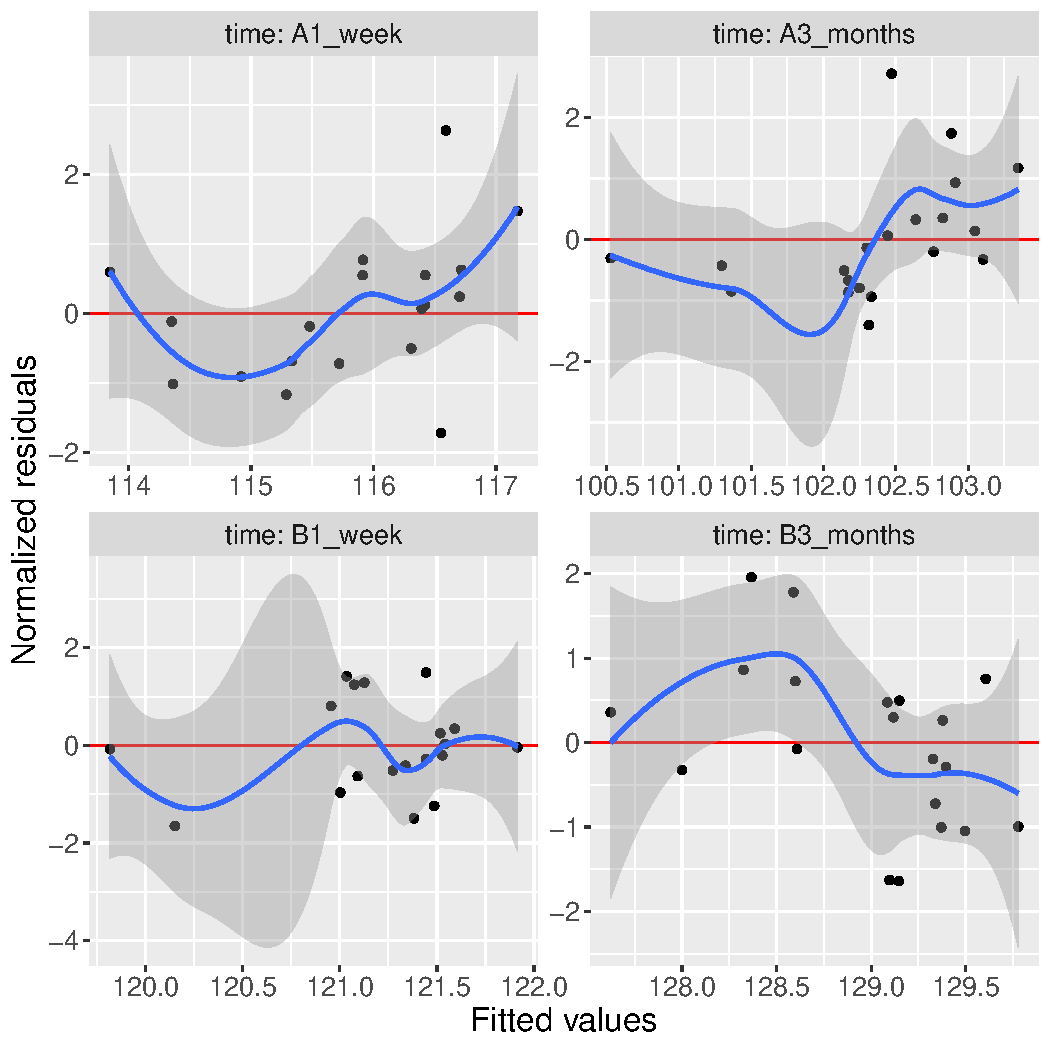
\includegraphics[width=0.4\textwidth]{./figures/diag-scatterplot.pdf}
\end{center}

\clearpage

\begin{itemize}
\item misspecification of the variance structure
\end{itemize}
\lstset{language=r,label= ,caption= ,captionpos=b,numbers=none}
\begin{lstlisting}
plot(eUN.lmm, type = "scatterplot2")
\end{lstlisting}

\begin{center}
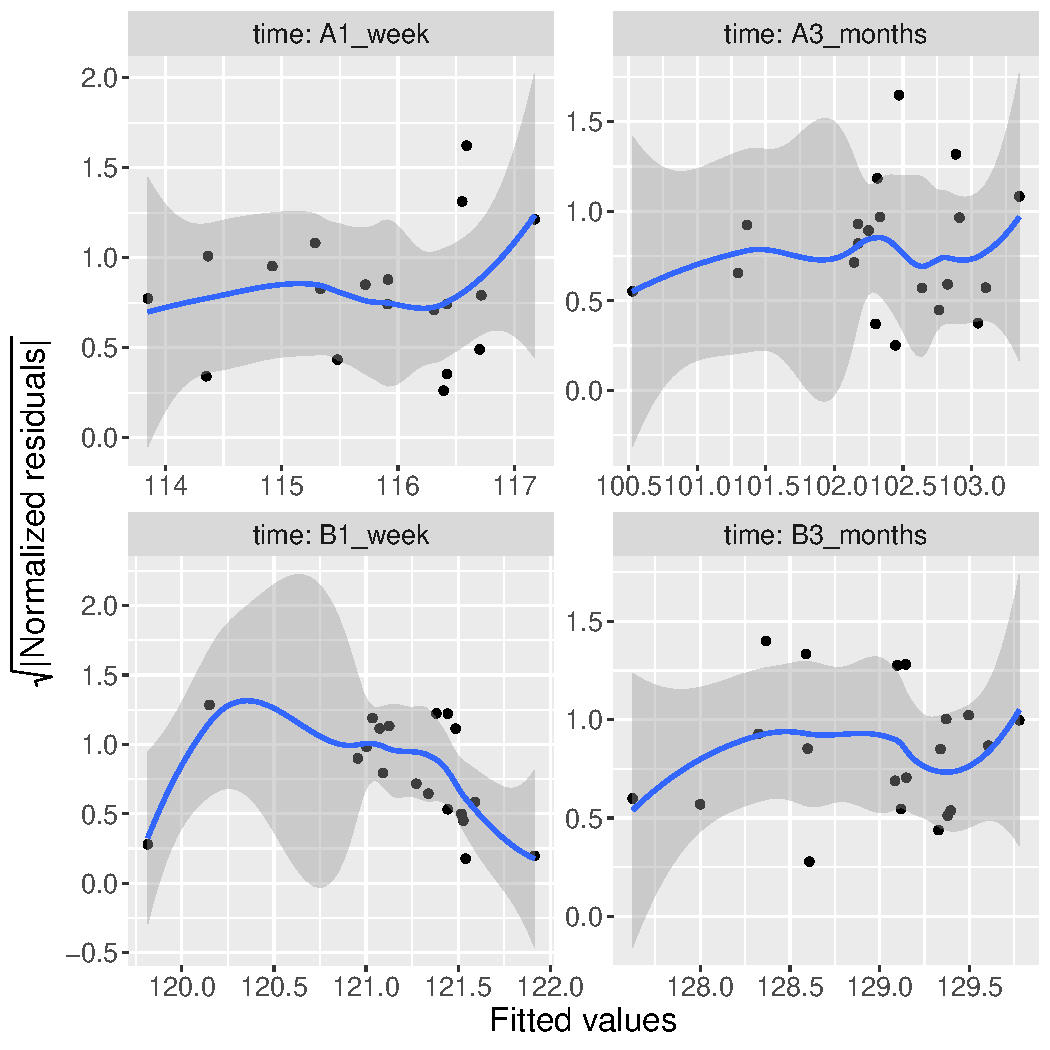
\includegraphics[width=0.4\textwidth]{./figures/diag-scatterplot2.pdf}
\end{center}

\begin{itemize}
\item misspecification of the correlation structure
\end{itemize}

\lstset{language=r,label= ,caption= ,captionpos=b,numbers=none}
\begin{lstlisting}
plot(eUN.lmm, type = "correlation", type.residual = "response")
plot(eUN.lmm, type = "correlation", type.residual = "normalized")
\end{lstlisting}

\begin{center}
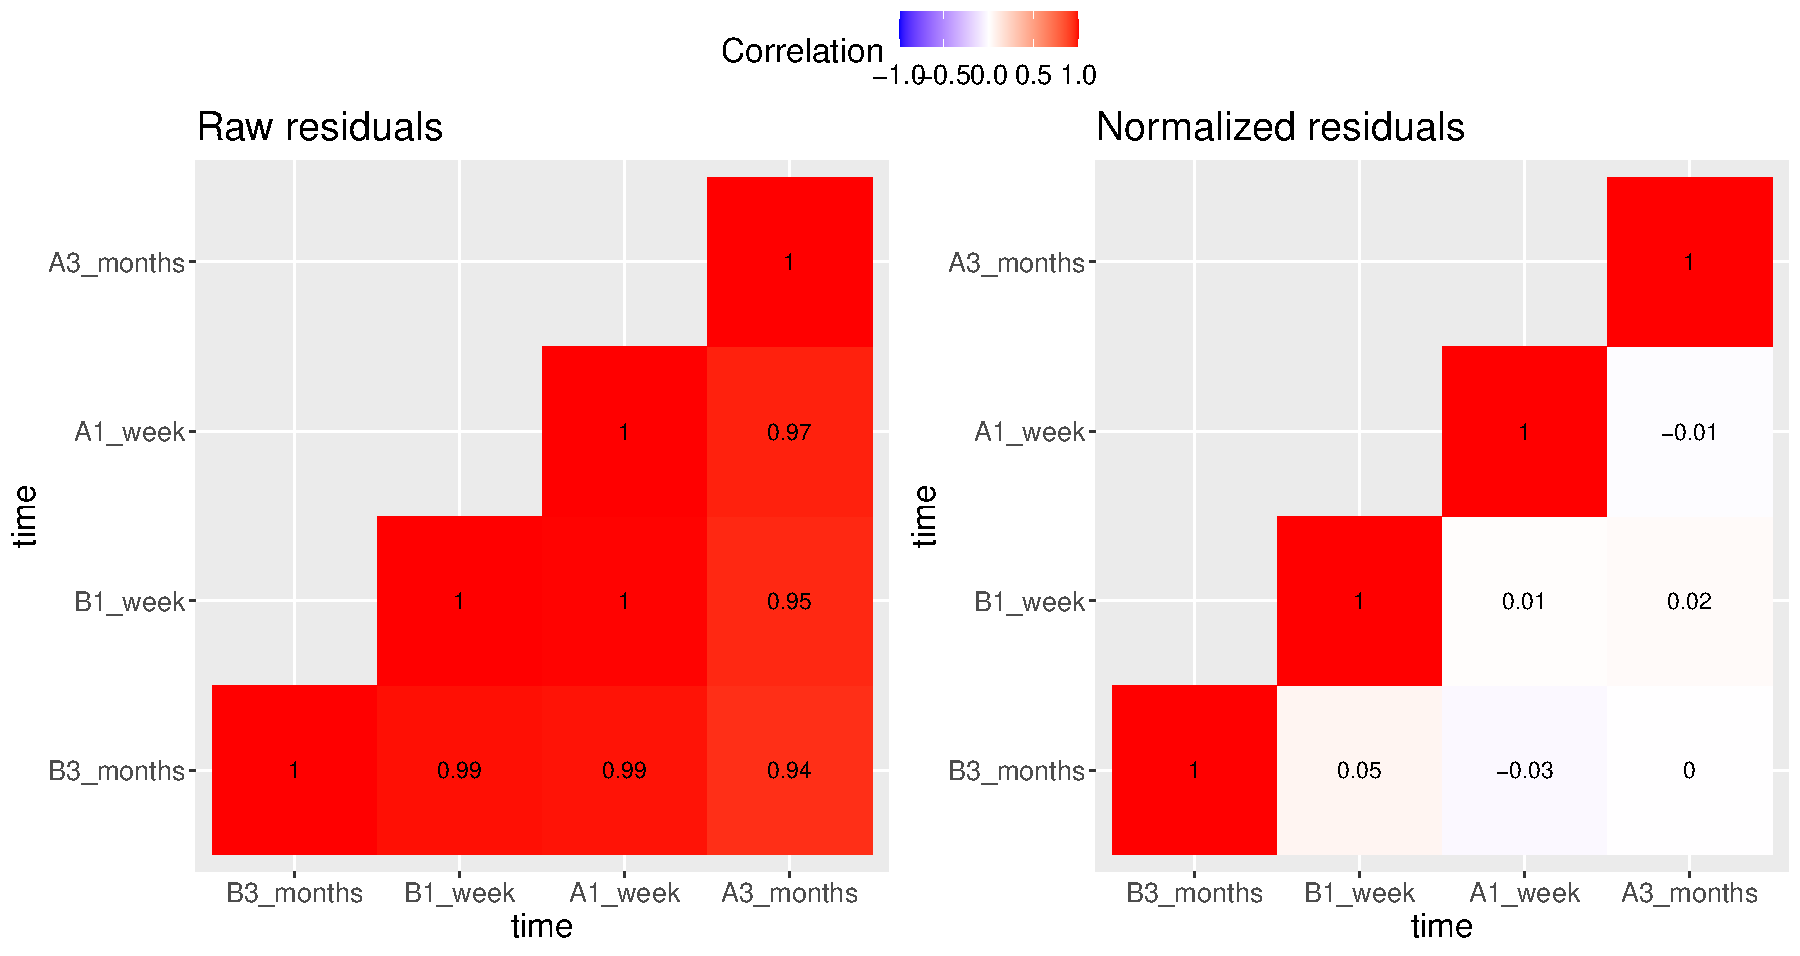
\includegraphics[width=0.6\textwidth]{./figures/diag-correlation.pdf}
\end{center}

\begin{itemize}
\item residual distribution vs. normal distribution \footnote{see \cite{oldford2016self} for guidance
about how to read quantile-quantile plots.}:
\end{itemize}
\lstset{language=r,label= ,caption= ,captionpos=b,numbers=none}
\begin{lstlisting}
plot(eUN.lmm, type = "qqplot", engine.qqplot = "qqtest")
## Note: the qqtest package to be installed to use the argument engine.plot = "qqtest" 
\end{lstlisting}

\begin{center}
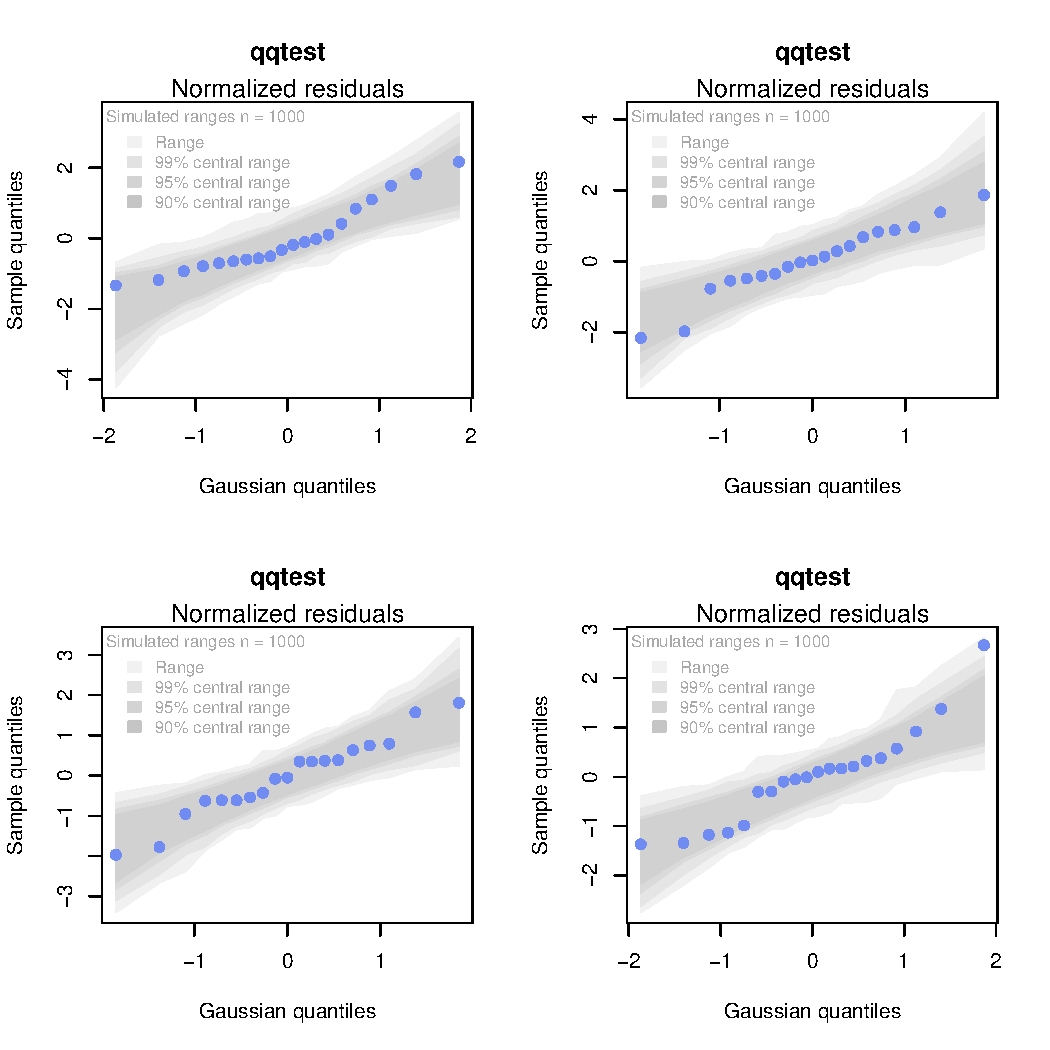
\includegraphics[width=0.5\textwidth]{./figures/diag-qqplot.pdf}
\end{center}

\Warning Deviation from the normal distribution does not necessarily
question the validity of the statistical inference. Moreover, for
variance and correlation parameters, normally distributed data is not
enought to ensure valid statistical inference. Instead one could
assess whether the log-likelihood is locally quadratic as this ensures
normally distributed estimates in finite samples
\citep{geyer2013asymptotics}. Since the likelihood function is a
multi-dimensional function this is not an easy task but one can look
at specific 'slices' using the \texttt{profile} method:

\lstset{language=r,label= ,caption= ,captionpos=b,numbers=none}
\begin{lstlisting}
plot(profile(eUN.lmm, effects = c("sigma","rho(B1w,A1w)")))
\end{lstlisting}


\begin{center}
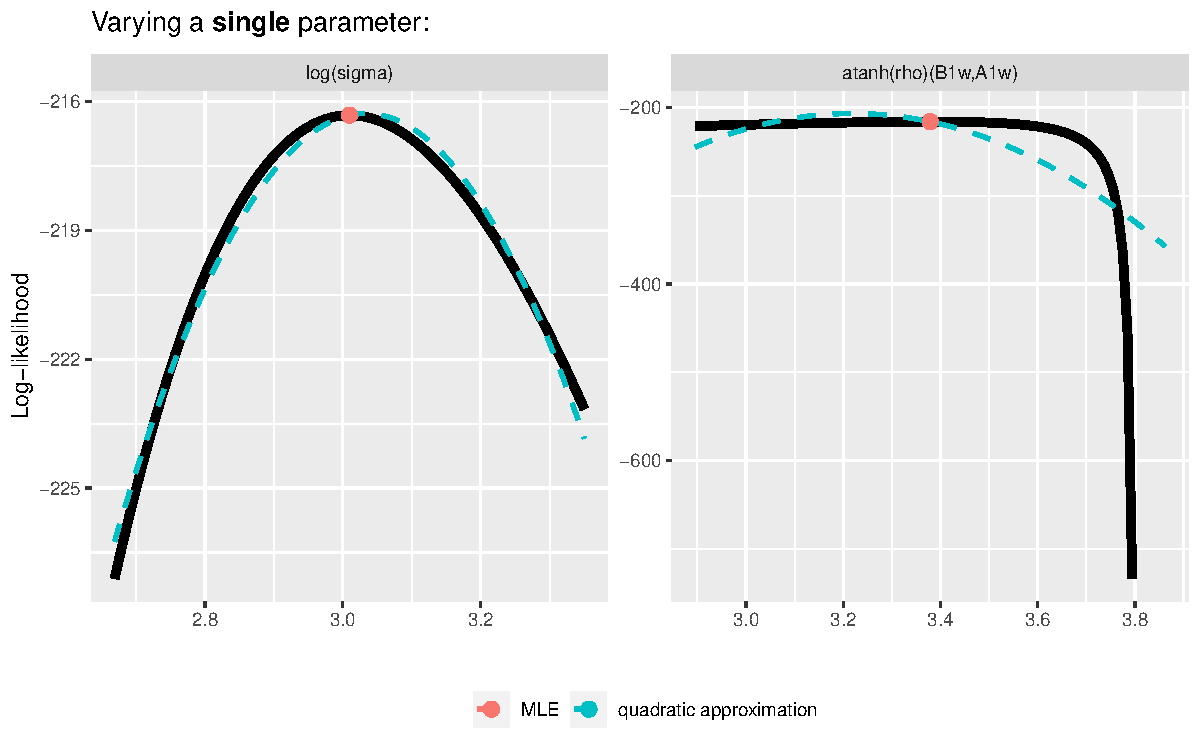
\includegraphics[width=0.5\textwidth]{./figures/diag-profileUN.pdf}
\end{center}

\clearpage

\subsection{Model fit}
\label{sec:org75ba3c5}

The fitted values can be displayed via the \texttt{plot} method or using the \texttt{emmeans} package:

\lstset{language=r,label= ,caption= ,captionpos=b,numbers=none}
\begin{lstlisting}
library(ggplot2) ## left panel
plot(eUN.lmm, type = "fit", color = "id", ci.alpha = NA, size.text = 20)
\end{lstlisting}

\lstset{language=r,label= ,caption= ,captionpos=b,numbers=none}
\begin{lstlisting}
library(emmeans) ## right panel
emmip(eUN.lmm, ~time) + theme(text = element_text(size=20))
\end{lstlisting}

\begin{minipage}{0.45\linewidth}
\begin{center}
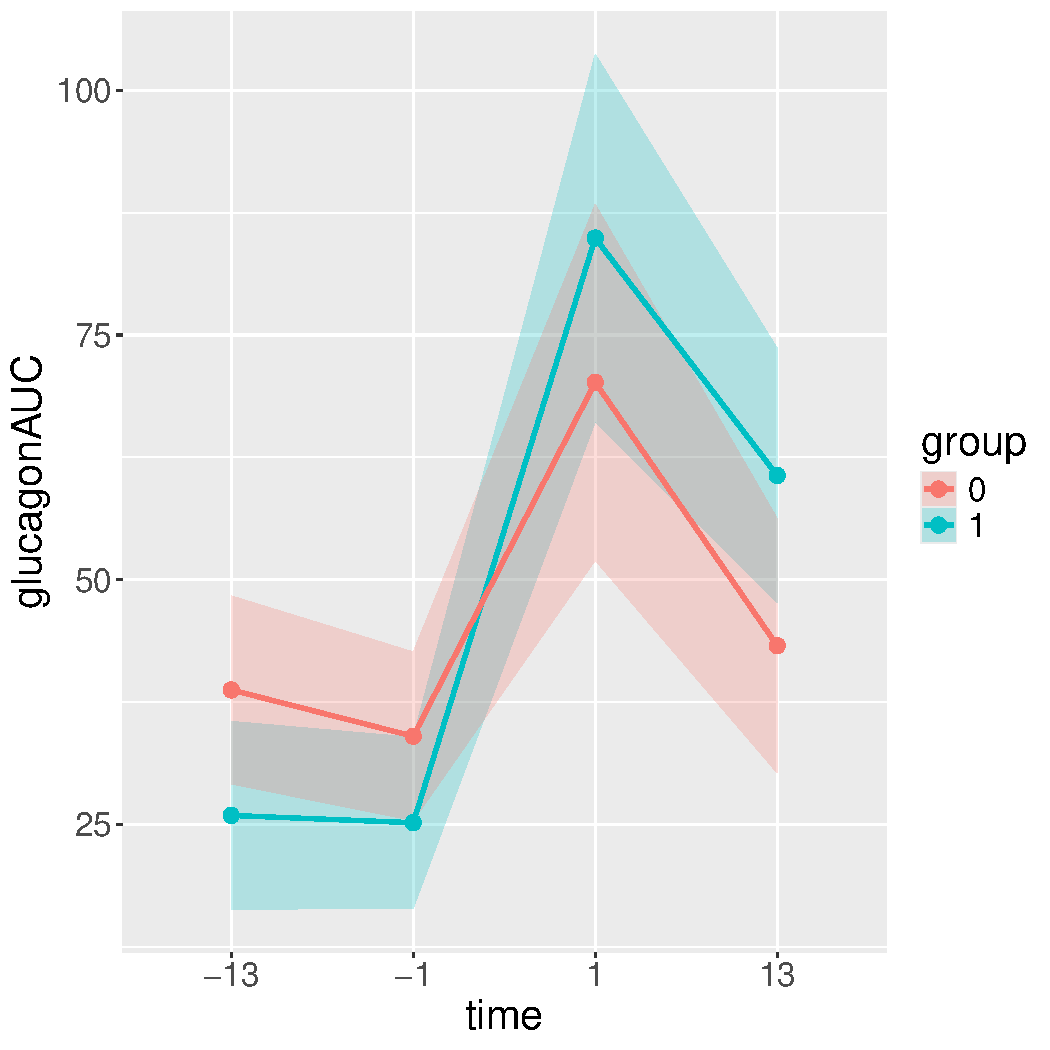
\includegraphics[width=\textwidth]{./figures/fit-autoplot.pdf}
\end{center}
\end{minipage}
\begin{minipage}{0.45\linewidth}
\begin{center}
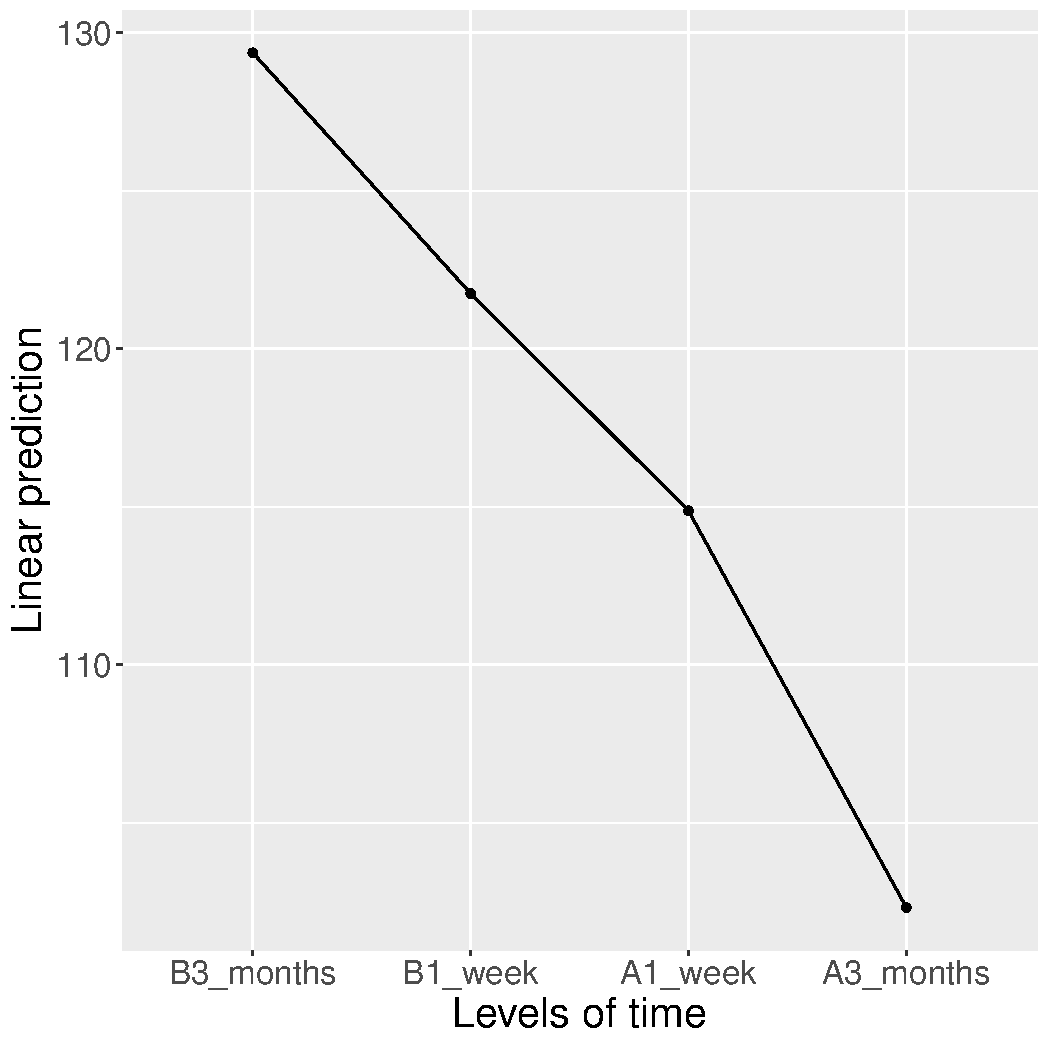
\includegraphics[width=\textwidth]{./figures/fit-emmip.pdf}
\end{center}
\end{minipage}

In the first case each possible curve is displayed while in the latter
the average curve (over glucagon values). With the \texttt{plot} method,
it is possible to display a curve specific to a glucagon value via the
argument \texttt{at}:
\lstset{language=r,label= ,caption= ,captionpos=b,numbers=none}
\begin{lstlisting}
## left panel
plot(eUN.lmm, type = "fit", at = data.frame(glucagon = 10), color = "glucagon") 
\end{lstlisting}

It is also possible to display the observed values along with the
fitted values by setting the argument \texttt{obs.alpha} to a strictly
positive value below or equal to 1. This argument controls the
transparency of the color used to display the observed values:
\lstset{language=r,label= ,caption= ,captionpos=b,numbers=none}
\begin{lstlisting}
## right panel
gg.spafit <- plot(eUN.lmm, type = "fit", obs.alpha = 0.25, ci = FALSE)$plot
\end{lstlisting}

\begin{minipage}{0.45\linewidth}
\begin{center}
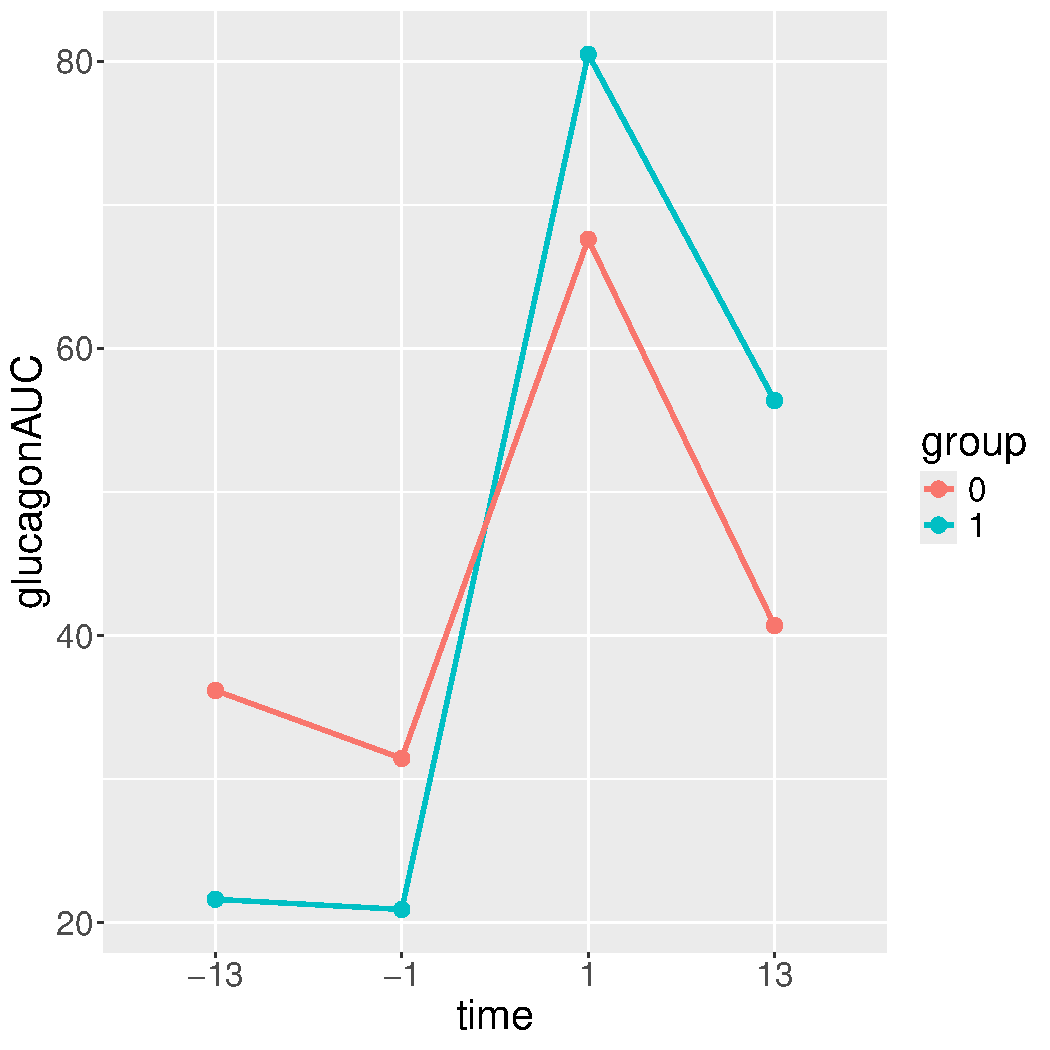
\includegraphics[width=\textwidth]{./figures/fit10-autoplot.pdf}
\end{center}
\end{minipage}
\begin{minipage}{0.45\linewidth}
\begin{center}
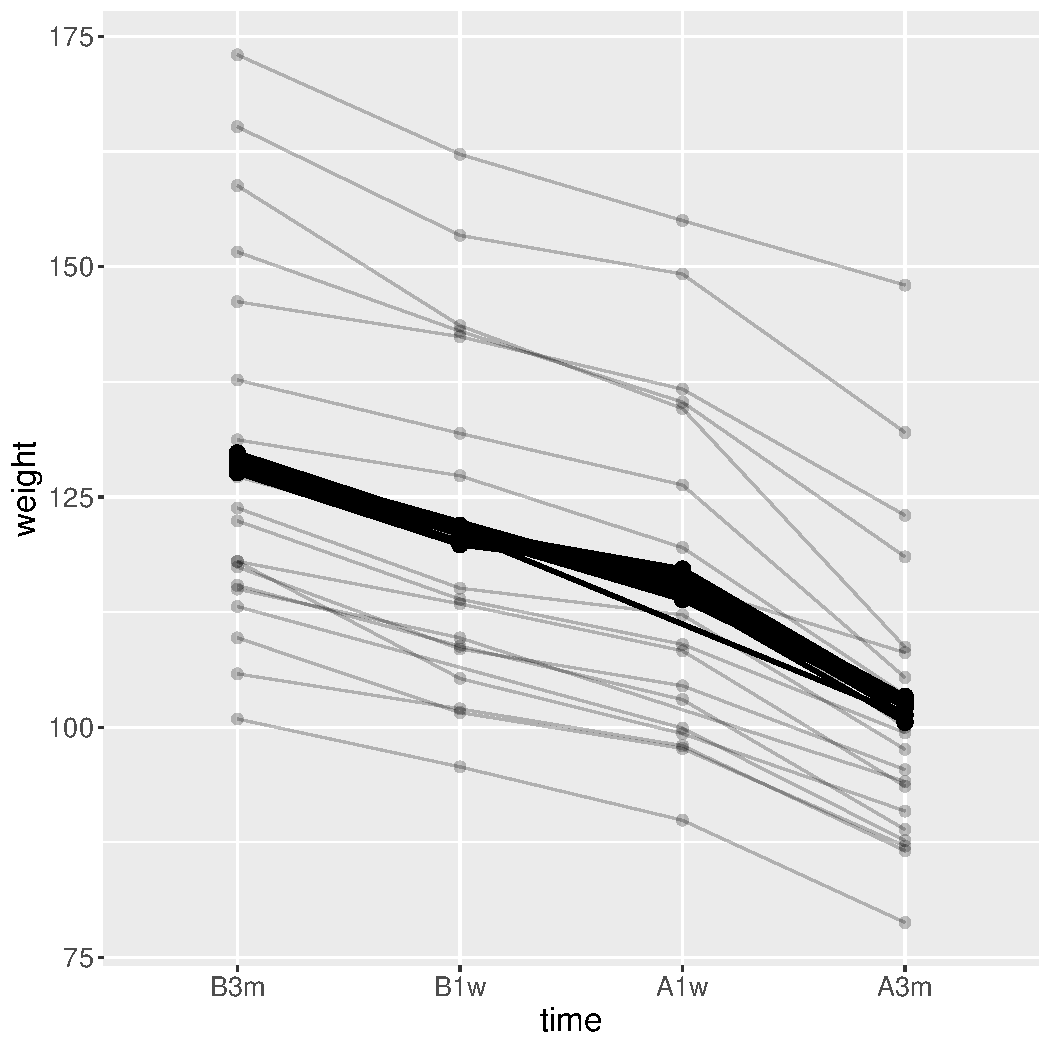
\includegraphics[width=\textwidth]{./figures/fitAll-autoplot.pdf}
\end{center}
\end{minipage}

The \texttt{plot} element output by the \texttt{plot} method can be manipulated as a ggplot object
to modify the visual appearance, e.g. to compare each individual
trajectory to the model fit:
\lstset{language=r,label= ,caption= ,captionpos=b,numbers=none}
\begin{lstlisting}
gg.traj <- gg.spafit + facet_wrap(~id, labeller = label_both)
gg.traj <- gg.traj + theme(axis.text.x=element_text(angle = 90, hjust = 0))
gg.traj
\end{lstlisting}

\begin{center}
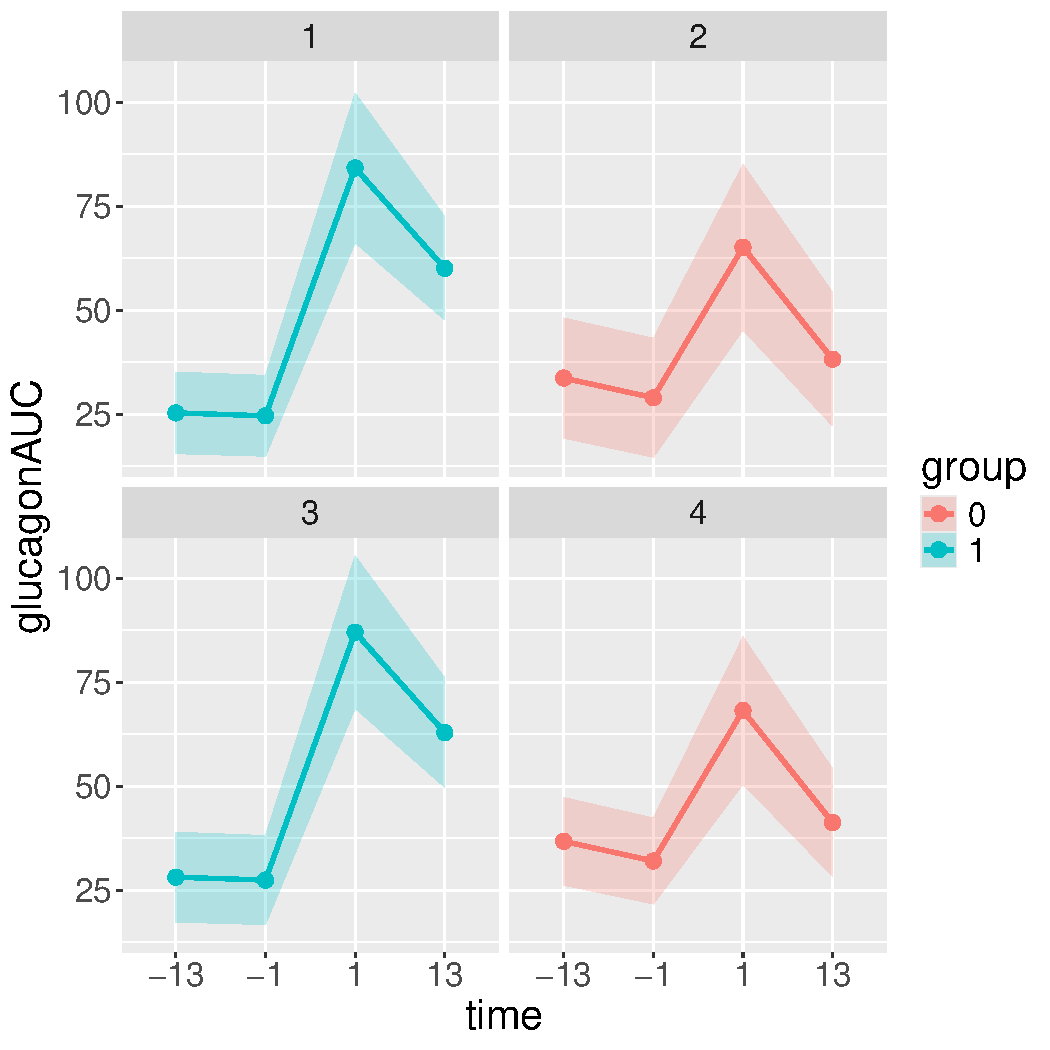
\includegraphics[width=\textwidth]{./figures/fit-autoplot-indiv.pdf}
\end{center}

\clearpage

\subsection{Partial residuals}
\label{sec:orge150da1}

Partial residuals can also be displayed via the \texttt{plot} method:
\lstset{language=r,label= ,caption= ,captionpos=b,numbers=none}
\begin{lstlisting}
gg1 <- plot(eUN.lmm, type = "partial", var = "glucagon")$plot
gg2 <- plot(eUN.lmm, type = "partial", var = c("(Intercept)","glucagon"))$plot
ggarrange(gg1,gg2)
\end{lstlisting}

\begin{center}
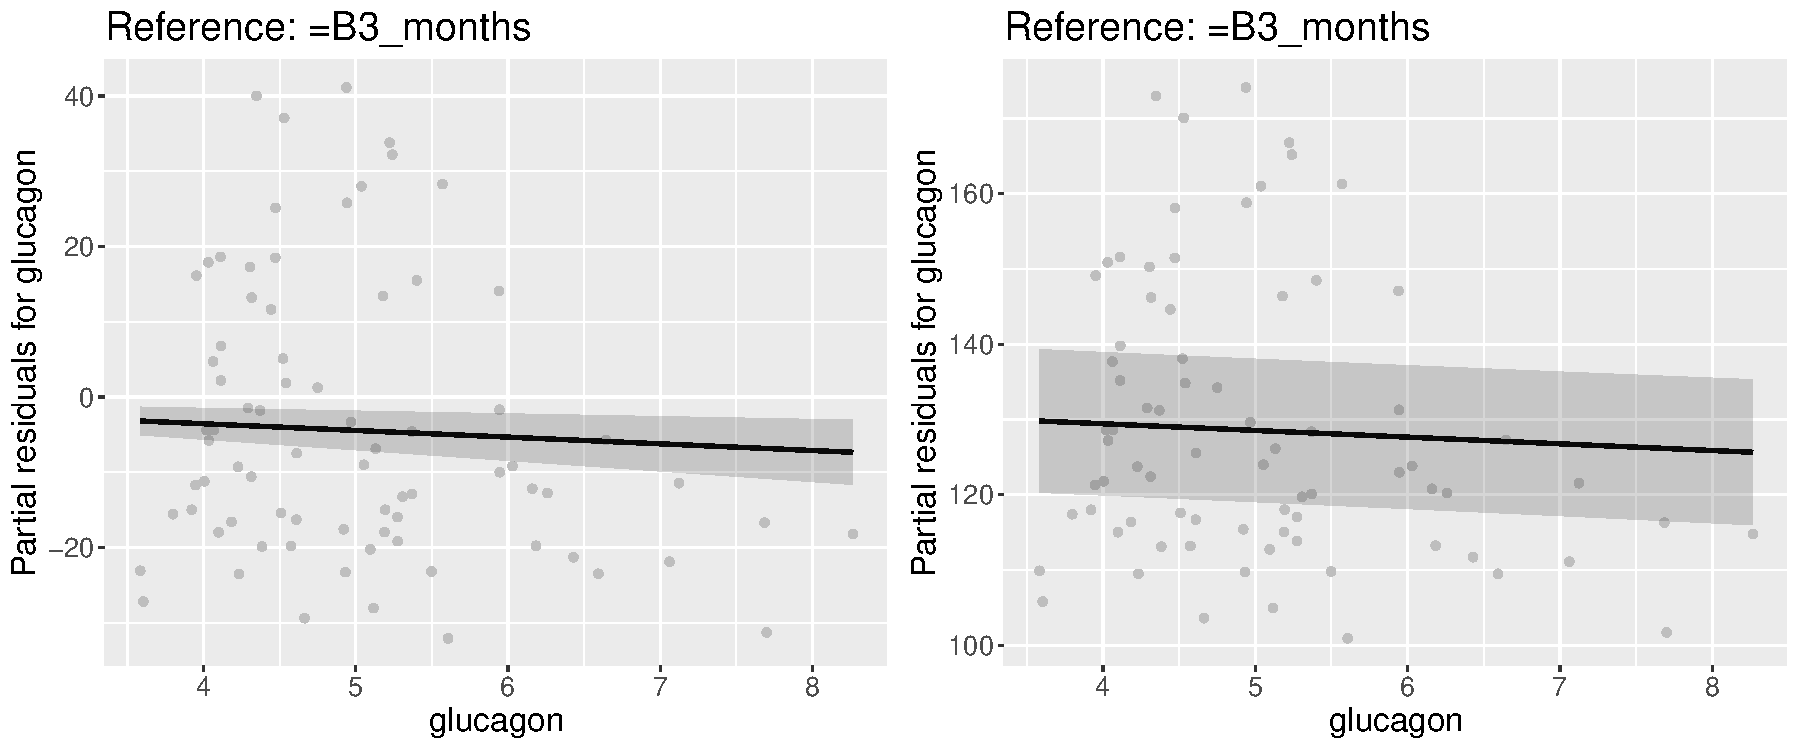
\includegraphics[width=0.75\textwidth]{./figures/fit-pres.pdf}
\end{center}

Their value can be extracted via the \texttt{residuals} method, e.g.:
\lstset{language=r,label= ,caption= ,captionpos=b,numbers=none}
\begin{lstlisting}
df.pres <- residuals(eUN.lmm, type = "partial", var = "glucagon", keep.data = TRUE)
head(df.pres)
\end{lstlisting}

\begin{verbatim}
  id visit time weight glucagonAUC baseline glucagon group    fitted  r.partial
1  1     1  B3m  127.2     5032.50     TRUE 4.034616     1 -3.583982  -5.780136
2  2     1  B3m  165.2    12142.50     TRUE 5.240766     0 -4.655415  32.219864
3  3     1  B3m  109.7    10321.35     TRUE 4.931824     1 -4.380979 -23.280136
4  4     1  B3m  146.2     6693.00     TRUE 4.316306     0 -3.834209  13.219864
5  5     1  B3m  113.1     7090.50     TRUE 4.383738     1 -3.894110 -19.880136
6  6     1  B3m  158.8    10386.00     TRUE 4.942791     0 -4.390721  25.819864
NULL
\end{verbatim}


This matches manual calculation:
\lstset{language=r,label= ,caption= ,captionpos=b,numbers=none}
\begin{lstlisting}
m.pres <- dfL$weight - model.matrix(~time,dfL) %*% coef(eUN.lmm)[1:4]
range(df.pres$r.partial - m.pres, na.rm = TRUE)

m.pfit <- model.matrix(~0+glucagon,dfL) %*% coef(eUN.lmm)["glucagon"]
range(df.pres$fitted - m.pfit, na.rm = TRUE)
\end{lstlisting}

\begin{verbatim}
[1] -1.421085e-14  1.421085e-14
[1] 0 0
\end{verbatim}


The \texttt{plot} methods can handle one continuous and one categorical
covariate (in addition to the intercept) to display interaction
plots. In that case each observation/fitted line is colored according
to the categorical covariate.

\clearpage

\subsection{Statistical inference (linear)}
\label{sec:org636ff5d}

The \texttt{anova} method can be use to test one or several linear
combinations of the model coefficients using Wald tests. By default,
it will simultaneously test all parameters associated to a variable:
\lstset{language=r,label= ,caption= ,captionpos=b,numbers=none}
\begin{lstlisting}
anova(eUN.lmm)
\end{lstlisting}

\begin{verbatim}
	     Multivariate Wald test 

               F-statistic       df  p.value    
mean: time          86.743 (3,19.0) 2.84e-11 ***
    : glucagon      13.518 (1,13.7)  0.00257  **
\end{verbatim}


Note that here the p-values are not adjust for multiple comparisons
over variables. It is possible to specify a null hypothesis to be
test: e.g. is there a change in average weight just after taking the
treatment:
\lstset{language=r,label= ,caption= ,captionpos=b,numbers=none}
\begin{lstlisting}
anova(eUN.lmm, effects = c("timeA1w-timeB1w=0"))
\end{lstlisting}

\begin{verbatim}
	     Multivariate Wald test 

       F-statistic       df  p.value    
all: 1      43.141 (1,17.9) 3.72e-06 ***
\end{verbatim}


One can also simulateneously tests several null hypotheses:
\lstset{language=r,label= ,caption= ,captionpos=b,numbers=none}
\begin{lstlisting}
e.anova <- anova(eUN.lmm, effects = c("timeA1w-timeB1w=0","timeA3m-timeB1w=0"))
summary(e.anova)
\end{lstlisting}

\begin{verbatim}
		Multivariate Wald test 

          F-statistic       df  p.value    
   all: 1      98.651 (2,18.6) 1.23e-10 ***
   ---------------------------------------- 
  Signif. codes:  0 '***' 0.001 '**' 0.01 '*' 0.05 '.' 0.1 ' ' 1.
  Degrees of freedom were computed using a Satterthwaite approximation (column df). 

		Univariate Wald test 

                     estimate    se   df   lower   upper p.value    
   timeA1w - timeB1w   -3.906 0.595 17.9  -5.329  -2.482  <1e-05 ***
   timeA3m - timeB1w   -18.24 1.323   19 -21.407 -15.073  <1e-05 ***
   --------------------------------------------------------------- 
  Signif. codes:  0 '***' 0.001 '**' 0.01 '*' 0.05 '.' 0.1 ' ' 1.
  Columns lower/upper/p.value adjusted for multiple comparisons -- max-test.
  (1e+05 samples have been used)
  Model-based standard errors are derived from the observed information (column se). 
  Degrees of freedom were computed using a Satterthwaite approximation (column df).
\end{verbatim}

\clearpage

or return all pairwise comparisons for a given factor using the \texttt{mcp}
function of the multcomp package:
\lstset{language=r,label= ,caption= ,captionpos=b,numbers=none}
\begin{lstlisting}
library(multcomp)
summary(anova(eUN.lmm, effects = mcp(time = "Tukey")))
\end{lstlisting}

\begin{verbatim}
Singular contrast matrix: contrasts "A1w - B1w" "A3m - B1w" "A3m - A1w" have been removed. 

		Multivariate Wald test 

             F-statistic       df  p.value    
   all: time      86.743 (3,19.0) 2.84e-11 ***
   ------------------------------------------- 
  Signif. codes:  0 '***' 0.001 '**' 0.01 '*' 0.05 '.' 0.1 ' ' 1.
  Degrees of freedom were computed using a Satterthwaite approximation (column df). 

		Univariate Wald test 

             estimate    se   df   lower   upper p.value    
   B1w - B3m   -7.882 0.713 19.2  -9.821  -5.944  <1e-05 ***
   A1w - B3m  -11.788 1.018 21.6 -14.554  -9.022  <1e-05 ***
   A3m - B3m  -26.122 1.656 18.8 -30.625  -21.62  <1e-05 ***
   A1w - B1w   -3.906 0.595 17.9  -5.522  -2.289  <1e-05 ***
   A3m - B1w   -18.24 1.323   19 -21.836 -14.644  <1e-05 ***
   A3m - A1w  -14.334 1.057 20.3 -17.206 -11.463  <1e-05 ***
   --------------------------------------------------------- 
  Signif. codes:  0 '***' 0.001 '**' 0.01 '*' 0.05 '.' 0.1 ' ' 1.
  Columns lower/upper/p.value adjusted for multiple comparisons -- max-test.
  (1e+05 samples have been used)
  Model-based standard errors are derived from the observed information (column se). 
  Degrees of freedom were computed using a Satterthwaite approximation (column df).
\end{verbatim}

Here the \texttt{summary} method prints not only the global test but also the
result associated to each hypothesis. When testing transformed
variance or correlation parameters, parentheses (as in \texttt{log(k).B1w})
cause problem for recognizing parameters:
\lstset{language=r,label= ,caption= ,captionpos=b,numbers=none}
\begin{lstlisting}
try(
  anova(eUN.lmm,
        effects = c("log(k).B1w=0","log(k).A1w=0","log(k).A3m=0"))
)
\end{lstlisting}

\begin{verbatim}
Error in .anova_Wald(object, effects = effects, robust = robust, rhs = rhs,  : 
  Possible mispecification of the argument 'effects' as running mulcomp::glht lead to the following error: 
Error in parse(text = ex[i]) : <text>:1:7: uventet symbol
1: log(k).B1w
          ^
\end{verbatim}


\clearpage

It is then advised to build a contrast matrix, e.g.:
\lstset{language=r,label= ,caption= ,captionpos=b,numbers=none}
\begin{lstlisting}
name.coef <- rownames(confint(eUN.lmm, effects = "all"))
name.varcoef <- grep("^k",name.coef, value = TRUE)
C <- matrix(0, nrow = 3, ncol = length(name.coef), dimnames = list(name.varcoef, name.coef))
diag(C[name.varcoef,name.varcoef]) <- 1
C[,1:9]
\end{lstlisting}

\begin{verbatim}
      (Intercept) timeB1w timeA1w timeA3m glucagon sigma k.B1w k.A1w k.A3m
k.B1w           0       0       0       0        0     0     1     0     0
k.A1w           0       0       0       0        0     0     0     1     0
k.A3m           0       0       0       0        0     0     0     0     1
\end{verbatim}


And then call the \texttt{anova} method specifying the null hypothesis via the
contrast matrix:
\lstset{language=r,label= ,caption= ,captionpos=b,numbers=none}
\begin{lstlisting}
anova(eUN.lmm, effects = C)
\end{lstlisting}

\begin{verbatim}
	     Multivariate Wald test 

       F-statistic       df p.value   
all: 1       6.203 (3,18.0) 0.00442 **
\end{verbatim}


Note that using the approach of \cite{pipper2012versatile} it is also
possible to adjust for multiple testing across several \texttt{lmm}
objects. To do so, one first fit the mixed models, then use the
\texttt{anova} method to indicate which hypotheses are being tested, and
combine them using \texttt{rbind}. Here is an (artificial) example:
\lstset{language=r,label= ,caption= ,captionpos=b,numbers=none}
\begin{lstlisting}
Manova <- rbind(anova(eInd.lmm, effects = "glucagon = 0"),
                anova(eCS.lmm, effects = "glucagon = 0"),
                anova(eUN.lmm, effects = "glucagon = 0"),
                name = c("Ind","CS","UN"))
summary(Manova) 
\end{lstlisting}

\begin{verbatim}
		Multivariate Wald test 

          Chi2-statistic      df  p.value    
   all: 1          6.393 (3,Inf) 0.000251 ***
   ------------------------------------------ 
  Signif. codes:  0 '***' 0.001 '**' 0.01 '*' 0.05 '.' 0.1 ' ' 1.

		Univariate Wald test 

                 estimate    se   df   lower  upper p.value   
   Ind: glucagon    -8.27 2.574 34.2 -14.403 -2.137 0.00395 **
   CS: glucagon     0.822  0.59 53.8  -0.584  2.228 0.40724   
   UN: glucagon    -0.888 0.353 13.7  -1.729 -0.047 0.03475  *
   ----------------------------------------------------------- 
  Signif. codes:  0 '***' 0.001 '**' 0.01 '*' 0.05 '.' 0.1 ' ' 1.
  Columns lower/upper/p.value adjusted for multiple comparisons -- max-test.
  (error when computing the adjusted columns lower/upper/p.value by numerical integration: 6.6e-05)
  Robust standard errors are derived from the observed information (column se).
\end{verbatim}

\clearpage

\subsection{Statistical inference (non-linear)}
\label{sec:org0bbcd84}

The \texttt{estimate} function can be used to test one or several non-linear
combinations of model coefficients, using a first order delta method
to quantify uncertainty. The combination has to be specified via a
function (argument \texttt{f}). To illustrate its use consider an ANCOVA
analysis:
\[ Y_{i1} = \textcolor{\darkred}{\alpha} + \textcolor{\darkblue}{\beta} Y_{i,0} + \textcolor{\darkgreen}{\gamma} X_{i} + e_{i} \]

\lstset{language=r,label= ,caption= ,captionpos=b,numbers=none}
\begin{lstlisting}
e.ANCOVA <- lm(weight4 ~ weight1 + group, data = gastricbypassW)
summary(e.ANCOVA)$coef
\end{lstlisting}

\begin{verbatim}
              Estimate Std. Error    t value     Pr(>|t|)
(Intercept) -5.9285136 8.78006389 -0.6752244 5.086140e-01
weight1      0.8236279 0.06411563 12.8459772 3.524665e-10
group        4.1404554 2.53335466  1.6343765 1.205604e-01
\end{verbatim}


We can replicate this analysis by first fitting a mixed model:
\[ Y_{ij} = \alpha_j + \gamma_j X_{i} + \varepsilon_{i,j} \text{ where } \varepsilon_i \sim \Gaus \left( \begin{bmatrix} 0 \\ 0 \end{bmatrix}, \begin{bmatrix} \sigma^2_1 & \rho \sigma_1 \sigma_2 \\ \rho \sigma_1 \sigma_2 & \sigma^2_2 \end{bmatrix} \right) \]
\lstset{language=r,label= ,caption= ,captionpos=b,numbers=none}
\begin{lstlisting}
dfL14 <- dfL[dfL$visit %in% c(1,4),]
dfL14$time <- droplevels(dfL14$time)
e.lmmANCOVA <- lmm(weight ~ time+time:group, repetition = ~time|id,
                   data = dfL14)
\end{lstlisting}

and then perform a first order delta-method:
\lstset{language=r,label= ,caption= ,captionpos=b,numbers=none}
\begin{lstlisting}
lava::estimate(e.lmmANCOVA, f = function(p){
  c(Y1 = as.double(p["rho(B3m,A3m)"]*p["k.A3m"]),
    X1 = as.double(p["timeA3m:group"]-p["rho(B3m,A3m)"]*p["k.A3m"]*p["timeB3m:group"]))
})
\end{lstlisting}

\begin{verbatim}
    estimate         se        df      lower     upper      p.value
Y1 0.8236279 0.06230919  9.874633  0.6845551 0.9627007 1.332743e-07
X1 4.1404554 2.46197819 15.161269 -1.1022695 9.3831803 1.130927e-01
\end{verbatim}


Indeed:
\begin{align*}
\Esp[Y_{i2}|Y_{i1},X_{i}] &= \alpha_2 + \gamma_2 X_{i} + \rho \frac{\sigma_2}{\sigma_1}\left(Y_{i1} - \alpha_1 - \gamma_1 X_{i}\right) \\
                         &= \textcolor{\darkred}{\alpha_2 - \rho \frac{\sigma_2}{\sigma_1} \alpha_1}
                         + \textcolor{\darkblue}{\rho \frac{\sigma_2}{\sigma_1}Y_{i1}}
                         + \textcolor{\darkgreen}{\left(\gamma_2 - \rho \frac{\sigma_2}{\sigma_1} \gamma_1\right)  X_{i} }
\end{align*}

We obtain identical estimate but different standard-errors/degrees of
freedom compared to the univariate linear model approach. The later is
to be prefer as it does not rely on approximation. The former is
nevertheless useful as it can handle missing data in the outcome
variable.

\clearpage

\subsection{Baseline adjustment}
\label{sec:org7c2402c}

In clinical trial the group and intervention variable often do not
coincide, e.g., in presence of baseline measurement. In our running
example, the first two measurement are pre-treatment (i.e. treatment
should be \texttt{"none"}) while the last two measurements are post-treatment
(i.e. treatment should be \texttt{1} or \texttt{2}). The \texttt{baselineAdjustment}
function can be helpful to:
\begin{itemize}
\item define the treatment variable from the time and allocation variable, where baseline has its specific value
\end{itemize}
\lstset{language=r,label= ,caption= ,captionpos=b,numbers=none}
\begin{lstlisting}
gastricbypassL$treat <- baselineAdjustment(gastricbypassL, variable = "group",
                                repetition = ~time|id, constrain = c("B3m","B1w"),
                                new.level = "none")
table(treat = gastricbypassL$treat, time = gastricbypassL$time, group = gastricbypassL$group)
\end{lstlisting}

\begin{verbatim}
, , group = 0

      time
treat  B3m B1w A1w A3m
  none  10  10   0   0
  0      0   0  10  10
  1      0   0   0   0

, , group = 1

      time
treat  B3m B1w A1w A3m
  none  10  10   0   0
  0      0   0   0   0
  1      0   0  10  10
\end{verbatim}

\begin{itemize}
\item define the treatment variable from the time and allocation variable,
where baseline corresponds to the reference group
\end{itemize}
\lstset{language=r,label= ,caption= ,captionpos=b,numbers=none}
\begin{lstlisting}
gastricbypassL$treat2 <- baselineAdjustment(gastricbypassL, variable = "group",
                                            repetition = ~time|id, constrain = c("B3m","B1w"))
table(treat = gastricbypassL$treat2, time = gastricbypassL$time, group = gastricbypassL$group)
\end{lstlisting}

\begin{verbatim}
, , group = 0

     time
treat B3m B1w A1w A3m
    1  10  10   0   0
    0   0   0  10  10

, , group = 1

     time
treat B3m B1w A1w A3m
    1  10  10  10  10
    0   0   0   0   0
\end{verbatim}

\begin{itemize}
\item define a time varying treatment variable from the time and allocation variable
\end{itemize}
\lstset{language=r,label= ,caption= ,captionpos=b,numbers=none}
\begin{lstlisting}
gastricbypassL$timeXtreat <- baselineAdjustment(gastricbypassL, variable = "group",
                                                repetition = ~time|id, constrain = c("B3m","B1w"),
                                                collapse.time = ".")

table(treat = gastricbypassL$timeXtreat, time = gastricbypassL$time, group = gastricbypassL$group)
\end{lstlisting}

\begin{verbatim}
, , group = 0

       time
treat   B3m B1w A1w A3m
  B3m    10   0   0   0
  B1w     0  10   0   0
  A1w.0   0   0  10   0
  A3m.0   0   0   0  10
  A1w.1   0   0   0   0
  A3m.1   0   0   0   0

, , group = 1

       time
treat   B3m B1w A1w A3m
  B3m    10   0   0   0
  B1w     0  10   0   0
  A1w.0   0   0   0   0
  A3m.0   0   0   0   0
  A1w.1   0   0  10   0
  A3m.1   0   0   0  10
\end{verbatim}

We would then typically like to model group differences only after
baseline (i.e. only at 1 week and 3 months after). This can be
performed using the time varying treatment variable, e.g.:
\lstset{language=r,label= ,caption= ,captionpos=b,numbers=none}
\begin{lstlisting}
eC.lmm <- lmm(weight ~ timeXtreat, data = gastricbypassL,
              repetition = ~time|id, structure = "UN")
coef(eC.lmm) ## change from baseline
\end{lstlisting}

\begin{verbatim}
(Intercept)   timeXtreatB1w timeXtreatA1w.0 timeXtreatA3m.0 timeXtreatA1w.1 timeXtreatA3m.1 
  128.97000        -7.73000       -13.38978       -28.52130       -13.15022       -24.68870
\end{verbatim}


or
\lstset{language=r,label= ,caption= ,captionpos=b,numbers=none}
\begin{lstlisting}
eC2.lmm <- lmm(weight ~ 0 + timeXtreat, data = gastricbypassL,
              repetition = ~time|id, structure = "UN")
coef(eC2.lmm) ## absolute value
\end{lstlisting}

\begin{verbatim}
timeXtreatB3m   timeXtreatB1w timeXtreatA1w.0 timeXtreatA3m.0 timeXtreatA1w.1 timeXtreatA3m.1 
     128.9700        121.2400        115.5802        100.4487        115.8198        104.2813
\end{verbatim}


The parametrization however does not (directly) output treatment
effects. Instead one may be tempted to use a formula like
\texttt{treatment*time}. However this will lead to a non-indentifiable
model. Indeed we are only able to estimate a total of 6 means when
constraining the expected baseline value between the two groups to be
the same. Therefore can at most identify 6 effects. However the design
matrix for the interaction model:
\lstset{language=r,label= ,caption= ,captionpos=b,numbers=none}
\begin{lstlisting}
colnames(model.matrix(weight ~ treat*time, data = gastricbypassL))
\end{lstlisting}

\begin{verbatim}
 [1] "(Intercept)"    "treat0"         "treat1"         "timeB1w"        "timeA1w"       
 [6] "timeA3m"        "treat0:timeB1w" "treat1:timeB1w" "treat0:timeA1w" "treat1:timeA1w"
[11] "treat0:timeA3m" "treat1:timeA3m"
\end{verbatim}


contains 12 parameters (i.e. 6 too many). Fortunately, the \texttt{lmm} will
 drop non-identifiable effects from the model and fit the resulting
 simplified model:
\lstset{language=r,label= ,caption= ,captionpos=b,numbers=none}
\begin{lstlisting}
eC3.lmm <- lmm(weight ~ treat2*time, data = gastricbypassL,
               repetition = ~time|id, structure = "UN")
\end{lstlisting}

\begin{verbatim}
Constant values in the design matrix for the mean structure.
Coefficients "treat20" "treat20:timeB1w" relative to interactions "treat2:time" have been removed.
\end{verbatim}


with the following coefficients:
\lstset{language=r,label= ,caption= ,captionpos=b,numbers=none}
\begin{lstlisting}
model.tables(eC3.lmm)
\end{lstlisting}

\begin{verbatim}
                   estimate        se       df      lower       upper      p.value
(Intercept)     128.9700000 4.5323695 18.98130 119.483009 138.4569911 0.000000e+00
timeB1w          -7.7300000 0.6974427 18.97552  -9.189892  -6.2701082 9.938186e-10
timeA1w         -13.1502219 0.8970429 22.87334 -15.006465 -11.2939786 4.058975e-13
timeA3m         -24.6886957 1.7751662 22.25061 -28.367762 -21.0096290 1.863398e-12
treat20:timeA1w  -0.2395562 0.6484895 17.66860  -1.603816   1.1247037 7.162149e-01
treat20:timeA3m  -3.8326086 2.1066817 17.60613  -8.265691   0.6004734 8.592047e-02
\end{verbatim}


One can vizualize the baseline adjustment via the \texttt{plot} function:
\lstset{language=r,label= ,caption= ,captionpos=b,numbers=none}
\begin{lstlisting}
plot(eC3.lmm, color = "group", ci = FALSE, size.text = 20, obs.alpha = 0.1)
\end{lstlisting}

\begin{center}
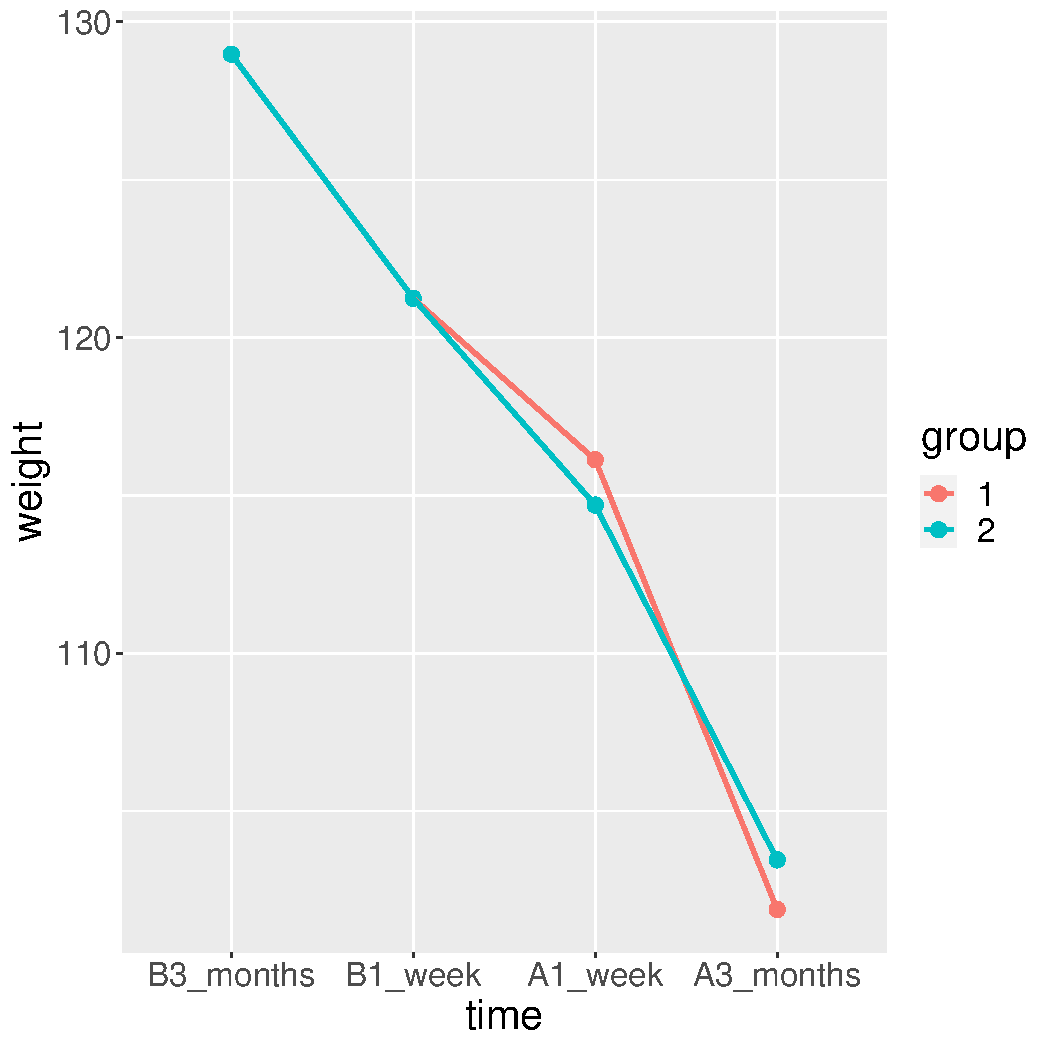
\includegraphics[width=0.4\textwidth]{./figures/gg-baseAdj.pdf}
\end{center}

\subsection{Marginal means}
\label{sec:org0860361}

The \texttt{emmeans} package can be used to output marginal means. Consider
the following model:
\lstset{language=r,label= ,caption= ,captionpos=b,numbers=none}
\begin{lstlisting}
dfL$group2 <- as.numeric(dfL$id) %% 3 == 0
e.group <- lmm(glucagon ~ time*group2, data = dfL,
               repetition = ~time|id, structure = "UN")
\end{lstlisting}

We can for instance compute the average value over time \emph{assuming balanced groups}:
\lstset{language=r,label= ,caption= ,captionpos=b,numbers=none}
\begin{lstlisting}
emmeans(e.group, specs=~time)
\end{lstlisting}

\begin{verbatim}
NOTE: Results may be misleading due to involvement in interactions
 time emmean    SE   df lower.CL upper.CL
 B3m    4.45 0.156 18.0     4.12     4.78
 B1w    4.32 0.131 18.0     4.05     4.60
 A1w    5.95 0.262 18.4     5.40     6.50
 A3m    5.12 0.187 18.0     4.73     5.51

Results are averaged over the levels of: group2 
Confidence level used: 0.95
\end{verbatim}


This differs from the average value over time over the whole sample:
\lstset{language=r,label= ,caption= ,captionpos=b,numbers=none}
\begin{lstlisting}
df.pred <- predict(e.group, newdata = dfL, keep.newdata = TRUE)
summarize(formula = estimate~time, data = df.pred)
\end{lstlisting}

\begin{verbatim}
  time observed missing     mean        sd      min       q1   median       q3      max
1  B3m       20       0 4.514352 0.1502565 4.290643 4.290643 4.610227 4.610227 4.610227
2  B1w       19       0 4.384638 0.1643256 4.149209 4.149209 4.493298 4.493298 4.493298
3  A1w       19       0 6.060587 0.2030009 5.729961 5.954314 6.178668 6.178668 6.178668
4  A3m       20       0 5.057642 0.1465315 4.964144 4.964144 4.964144 5.275805 5.275805
\end{verbatim}


as the groups are not balanced:
\lstset{language=r,label= ,caption= ,captionpos=b,numbers=none}
\begin{lstlisting}
table(group = dfL$group2, time = dfL$time)
\end{lstlisting}

\begin{verbatim}
       time
group   B3m B1w A1w A3m
  FALSE  14  13  14  14
  TRUE    6   6   5   6
\end{verbatim}


The "emmeans" approach gives equal "weight" to the expected value of
both group:
\lstset{language=r,label= ,caption= ,captionpos=b,numbers=none}
\begin{lstlisting}
mu.group1 <-  as.double(coef(e.group)["(Intercept)"])
mu.group2 <-  as.double(coef(e.group)["(Intercept)"] + coef(e.group)["group2TRUE"])
p.group1 <- 14/20          ; p.group2 <- 6/20
c(emmeans = (mu.group1+mu.group2)/2, predict = mu.group1 * p.group1 + mu.group2 * p.group2)
\end{lstlisting}

\begin{verbatim}
 emmeans  predict 
4.450435 4.514352
\end{verbatim}


Which one is relevant depends on the application. The \texttt{emmeans}
function can also be used to display expected value in each group over
time:
\lstset{language=r,label= ,caption= ,captionpos=b,numbers=none}
\begin{lstlisting}
emmeans.group <- emmeans(e.group, specs = ~group2|time)
emmeans.group
\end{lstlisting}

\begin{verbatim}
time = B3m:
 group2 emmean    SE   df lower.CL upper.CL
 FALSE    4.61 0.171 18.0     4.25     4.97
  TRUE    4.29 0.262 18.0     3.74     4.84

time = B1w:
 group2 emmean    SE   df lower.CL upper.CL
 FALSE    4.49 0.145 18.4     4.19     4.80
  TRUE    4.15 0.219 17.9     3.69     4.61

time = A1w:
 group2 emmean    SE   df lower.CL upper.CL
 FALSE    6.18 0.277 17.8     5.60     6.76
  TRUE    5.73 0.446 18.6     4.80     6.66

time = A3m:
 group2 emmean    SE   df lower.CL upper.CL
 FALSE    4.96 0.205 18.0     4.53     5.39
  TRUE    5.28 0.313 18.0     4.62     5.93

Confidence level used: 0.95
\end{verbatim}

\clearpage

Using the \texttt{pair} function displays the differences:
\lstset{language=r,label= ,caption= ,captionpos=b,numbers=none}
\begin{lstlisting}
epairs.group <- pairs(emmeans.group, reverse = TRUE)
epairs.group
\end{lstlisting}

\begin{verbatim}
time = B3m:
 contrast     estimate    SE   df t.ratio p.value
 TRUE - FALSE   -0.320 0.313 18.0  -1.022  0.3202

time = B1w:
 contrast     estimate    SE   df t.ratio p.value
 TRUE - FALSE   -0.344 0.262 18.0  -1.311  0.2062

time = A1w:
 contrast     estimate    SE   df t.ratio p.value
 TRUE - FALSE   -0.449 0.525 18.4  -0.855  0.4034

time = A3m:
 contrast     estimate    SE   df t.ratio p.value
 TRUE - FALSE    0.312 0.374 18.0   0.834  0.4153
\end{verbatim}

One can adjust for multiple comparison via the \texttt{adjust} argument and
display confidence intervals setting the argument \texttt{infer} to \texttt{TRUE}:
\lstset{language=r,label= ,caption= ,captionpos=b,numbers=none}
\begin{lstlisting}
summary(epairs.group, by = NULL, adjust = "mvt", infer = TRUE)
\end{lstlisting}

\begin{verbatim}
 contrast     time estimate    SE   df lower.CL upper.CL t.ratio p.value
 TRUE - FALSE B3m    -0.320 0.313 18.0    -1.16    0.518  -1.022  0.6928
 TRUE - FALSE B1w    -0.344 0.262 18.0    -1.05    0.359  -1.311  0.5066
 TRUE - FALSE A1w    -0.449 0.525 18.4    -1.86    0.958  -0.855  0.7961
 TRUE - FALSE A3m     0.312 0.374 18.0    -0.69    1.314   0.834  0.8085

Confidence level used: 0.95 
Conf-level adjustment: mvt method for 4 estimates 
P value adjustment: mvt method for 4 tests
\end{verbatim}


This should also work when doing baseline adjustment (because of
baseline adjustment no difference is expected at the first two
timepoints):
\lstset{language=r,label= ,caption= ,captionpos=b,numbers=none}
\begin{lstlisting}
summary(pairs(emmeans(eC3.lmm , specs = ~treat2|time), reverse = TRUE), by = NULL)
\end{lstlisting}

\begin{verbatim}
Note: adjust = "tukey" was changed to "sidak"
because "tukey" is only appropriate for one set of pairwise comparisons
 contrast          time estimate    SE  df t.ratio p.value
 treat20 - treat21 B3m      0.00 0.000 Inf     NaN     NaN
 treat20 - treat21 B1w      0.00 0.000 Inf     NaN     NaN
 treat20 - treat21 A1w     -0.24 0.648  18  -0.369  0.9935
 treat20 - treat21 A3m     -3.83 2.107  18  -1.819  0.3019

P value adjustment: sidak method for 4 tests
\end{verbatim}


\clearpage

\subsection{Predictions}
\label{sec:org96eff1e}

Two types of predictions can be performed with the \texttt{predict} method:
\begin{itemize}
\item \textbf{static predictions} that are only conditional on the covariates:
\end{itemize}
\lstset{language=r,label= ,caption= ,captionpos=b,numbers=none}
\begin{lstlisting}
news <- dfL[dfL$id==1,]
news$glucagon <- 0
predict(eUN.lmm, newdata = news)
\end{lstlisting}

\begin{verbatim}
  estimate       se       df     lower    upper
1 132.9801 4.664247 19.75815 123.24305 142.7172
2 125.0979 4.388294 19.91418 115.94155 134.2543
3 121.1922 4.214230 20.55331 112.41660 129.9678
4 106.8577 3.942058 20.95499  98.65871 115.0568
\end{verbatim}


which can be computing by creating a design matrix:
\lstset{language=r,label= ,caption= ,captionpos=b,numbers=none}
\begin{lstlisting}
X.12 <- model.matrix(formula(eUN.lmm), news)
X.12
\end{lstlisting}

\begin{verbatim}
   (Intercept) timeB1w timeA1w timeA3m glucagon
1            1       0       0       0        0
21           1       1       0       0        0
41           1       0       1       0        0
61           1       0       0       1        0
attr(,"assign")
[1] 0 1 1 1 2
attr(,"contrasts")
attr(,"contrasts")$time
[1] "contr.treatment"
\end{verbatim}

and then multiplying it with the regression coefficients:
\lstset{language=r,label= ,caption= ,captionpos=b,numbers=none}
\begin{lstlisting}
X.12 %*% coef(eUN.lmm)
\end{lstlisting}

\begin{verbatim}
       [,1]
1  132.9801
21 125.0979
41 121.1922
61 106.8577
\end{verbatim}


\clearpage

\begin{itemize}
\item \textbf{dynamic predictions} that are conditional on the covariates and the
outcome measured at other timepoints. Consider two subjects for who
we would like to predict the weight 1 week before the intervention
based on the weight 3 months before the intervention:
\end{itemize}

\lstset{language=r,label= ,caption= ,captionpos=b,numbers=none,otherkeywords={}, deletekeywords={}}
\begin{lstlisting}
newd <- rbind(
  data.frame(id = 1, time = "B3m", weight = coef(eUN.lmm)["(Intercept)"], glucagon = 0),
  data.frame(id = 1, time = "B1w", weight = NA, glucagon = 0),
  data.frame(id = 2, time = "B3m", weight = 100, glucagon = 0),
  data.frame(id = 2, time = "B1w", weight = NA, glucagon = 0)
)
predict(eUN.lmm, newdata = newd, type = "dynamic", keep.newdata = TRUE)
\end{lstlisting}

\begin{verbatim}
  id time   weight glucagon  estimate        se  df     lower    upper
1  1  B3m 132.9801        0        NA        NA Inf        NA       NA
2  1  B1w       NA        0 125.09790 0.6362754 Inf 123.85083 126.3450
3  2  B3m 100.0000        0        NA        NA Inf        NA       NA
4  2  B1w       NA        0  94.47017 7.2279385 Inf  80.30367 108.6367
\end{verbatim}


The first subjects has the average weight while the second has a much
  lower weight. The predicted weight for the first subject is then the
  average weight one week before while it is lower for the second
  subject due to the positive correlation over time. The predicted
  value is computed using the formula of the conditional mean for a
  Gaussian vector:
\lstset{language=r,label= ,caption= ,captionpos=b,numbers=none}
\begin{lstlisting}
mu1 <- coef(eUN.lmm)[1]
mu2 <- sum(coef(eUN.lmm)[1:2])
Omega_11 <- sigma(eUN.lmm)["B3m","B3m"]
Omega_21 <- sigma(eUN.lmm)["B1w","B3m"]
as.double(mu2 + Omega_21 * (100 - mu1) / Omega_11)
\end{lstlisting}

\begin{verbatim}
[1] 94.47017
\end{verbatim}



\clearpage

\section{Equivalence with other statistical methods}
\label{sec:orge17d74b}
\subsection{T-test}
\label{sec:org2ff7a25}
A t-test:
\lstset{language=r,label= ,caption= ,captionpos=b,numbers=none}
\begin{lstlisting}
t.test(weight4 ~ group, data = gastricbypassW)
\end{lstlisting}

\begin{verbatim}

	Welch Two Sample t-test

data:  weight4 by group
t = 0.59144, df = 17.679, p-value = 0.5617
alternative hypothesis: true difference in means between group 0 and group 1 is not equal to 0
95 percent confidence interval:
 -11.73582  20.91582
sample estimates:
mean in group 0 mean in group 1 
         104.66          100.07
\end{verbatim}

is equivalent to an independent covariance pattern with a different
variable for each group:
\lstset{language=r,label= ,caption= ,captionpos=b,numbers=none}
\begin{lstlisting}
e.ttest4 <- lmm(weight4 ~ group, structure = IND(~group), 
               data = gastricbypassW, trace = FALSE)
model.tables(e.ttest4)
\end{lstlisting}

\begin{verbatim}
            estimate       se       df     lower     upper      p.value
(Intercept)   104.66 5.104469  9.00180  93.11324 116.20676 7.270954e-09
group          -4.59 7.760674 17.68244 -20.91558  11.73558 5.617090e-01
\end{verbatim}


Multiple t-tests:
\lstset{language=r,label= ,caption= ,captionpos=b,numbers=none}
\begin{lstlisting}
e.ttest1 <- lmm(weight1 ~ group, structure = IND(~group), 
                data = gastricbypassW, trace = FALSE)
e.ttest2 <- lmm(weight2 ~ group, structure = IND(~group), 
                data = gastricbypassW, trace = FALSE)
e.ttest3 <- lmm(weight3 ~ group, structure = IND(~group), 
                data = gastricbypassW, trace = FALSE)
\end{lstlisting}

can be adjusted for multiple comparison by first using the \texttt{anova}
function to specify the parameter of interest and combining the
results using \texttt{rbind}:
\lstset{language=r,label= ,caption= ,captionpos=b,numbers=none}
\begin{lstlisting}
e.mttest <- rbind(anova(e.ttest1, effects = "group=0"),
                  anova(e.ttest2, effects = "group=0"),
                  anova(e.ttest3, effects = "group=0"),
                  anova(e.ttest4, effects = "group=0"))
model.tables(e.mttest, method = "bonferroni")
\end{lstlisting}

\begin{verbatim}
               estimate       se       df     lower    upper p.value
weight1: group   -10.60 8.971747 17.96464 -35.49775 14.29775       1
weight2: group    -9.50 8.395143 17.98540 -32.79464 13.79464       1
weight3: group    -8.92 8.129458 17.95876 -31.48110 13.64110       1
weight4: group    -4.59 7.760674 17.68244 -26.16472 16.98472       1
\end{verbatim}


\Warning efficient adjustment for multiple comparisons (like
\texttt{"single-step"}) will not be valid as the correlation structure has
not be specified. To do so it is more conveniently to work with a the
long format:
\lstset{language=r,label= ,caption= ,captionpos=b,numbers=none}
\begin{lstlisting}
e.mttest2 <- mlmm(weight ~ group, structure = IND(~group),
                  data = gastricbypassL, trace = FALSE,
                  effects = "group=0", by = "time", repetition = ~time|id)
model.tables(e.mttest2, method = "single-step2")
\end{lstlisting}

\begin{verbatim}
   by parameter estimate       se       df     lower     upper   p.value
1 B3m     group   -10.60 8.971747 17.96464 -30.89407  9.694068 0.3155368
2 B1w     group    -9.50 8.395143 17.98540 -28.48979  9.489791 0.3387166
3 A1w     group    -8.92 8.129458 17.95876 -27.30881  9.468813 0.3554664
4 A3m     group    -4.59 7.760674 17.68244 -22.14462 12.964624 0.6640334
\end{verbatim}


or call the dedicated function \texttt{mt.test}:
\lstset{language=r,label= ,caption= ,captionpos=b,numbers=none}
\begin{lstlisting}
mt.test(weight1+weight2+weight3+weight4~group, data = gastricbypassW)
\end{lstlisting}

\begin{verbatim}
       by parameter estimate       se       df     lower     upper   p.value
1 weight1     group   -10.60 8.971747 17.96464 -30.97670  9.776698 0.3197968
2 weight2     group    -9.50 8.395143 17.98540 -28.56711  9.567110 0.3423566
3 weight3     group    -8.92 8.129458 17.95876 -27.38368  9.543685 0.3584364
4 weight4     group    -4.59 7.760674 17.68244 -22.21610 13.036099 0.6649434
\end{verbatim}

\subsection{Linear regression on the change}
\label{sec:orgb48e702}

A widely spread approach to analyze longitudinal data is to reduce the
number of repetitions to 1 by working on the change and then apply
'usual' statistical methods. For instance one could compare the pre-
and post- operation values using:

\lstset{language=r,label= ,caption= ,captionpos=b,numbers=none}
\begin{lstlisting}
gastricbypassW$changeG41 <- gastricbypassW$glucagonAUC4-gastricbypassW$glucagonAUC1
e.change41 <- lm(changeG41 ~ weight1, data = gastricbypassW)
summary(e.change41)$coef
\end{lstlisting}

\begin{verbatim}
             Estimate Std. Error   t value   Pr(>|t|)
(Intercept) 17865.953 9292.61106  1.922598 0.07050076
weight1      -113.696   71.22173 -1.596367 0.12781371
\end{verbatim}


\clearpage

This turns out to be equivalent to the following mixed model:
\lstset{language=r,label= ,caption= ,captionpos=b,numbers=none}
\begin{lstlisting}
gastricbypassL41 <- gastricbypassL[gastricbypassL$visit %in% c(1,4),]
gastricbypassL41$time <- droplevels(gastricbypassL41$time)
gastricbypassL41$weight1 <- gastricbypassW$weight1[gastricbypassL41$id]

e.lmm41 <- lmm(glucagonAUC ~ time + time*weight1,
               repetition =~ time|id, structure = "UN",
               data = gastricbypassL41)
model.tables(e.lmm41)
\end{lstlisting}

\begin{verbatim}
                    estimate         se       df       lower       upper    p.value
(Intercept)      7730.051990 5737.22268 18.00298 -4323.26268 19783.36666 0.19458155
timeA3m         17865.953183 9292.61106 18.00104 -1657.01749 37388.92385 0.07049983
weight1             1.011014   43.97202 18.00298   -91.36968    93.39171 0.98190941
timeA3m:weight1  -113.695981   71.22173 18.00104  -263.32666    35.93469 0.12781271
\end{verbatim}


This equivalence only holds as there is no missing data.
\lstset{language=r,label= ,caption= ,captionpos=b,numbers=none}
\begin{lstlisting}
index.missing41 <- which(is.na(gastricbypassW$changeG41))
index.missing41
\end{lstlisting}

\begin{verbatim}
integer(0)
\end{verbatim}

\subsection{Correlation between changes}
\label{sec:orgf8a6238}

In some studies, one is interested in studying the relation between
two evolutions. Say weight and glucagon before and after the
operation:
\lstset{language=r,label= ,caption= ,captionpos=b,numbers=none}
\begin{lstlisting}
gastricbypassW$changeG41 <- gastricbypassW$glucagonAUC4-gastricbypassW$glucagonAUC1
gastricbypassW$changeW41 <- gastricbypassW$weight4-gastricbypassW$weight1
\end{lstlisting}

\clearpage

One can evaluate their correlation:
\lstset{language=r,label= ,caption= ,captionpos=b,numbers=none}
\begin{lstlisting}
cor.test(gastricbypassW$changeW41, gastricbypassW$changeG41)
\end{lstlisting}

\begin{verbatim}

	Pearson's product-moment correlation

data:  gastricbypassW$changeW41 and gastricbypassW$changeG41
t = 1.8667, df = 18, p-value = 0.07831
alternative hypothesis: true correlation is not equal to 0
95 percent confidence interval:
 -0.0484149  0.7174011
sample estimates:
      cor 
0.4027343
\end{verbatim}

or regress one against the other:
\lstset{language=r,label= ,caption= ,captionpos=b,numbers=none}
\begin{lstlisting}
e2.change41 <- lm(changeG41 ~ changeW41, data = gastricbypassW)
summary(e2.change41)$coef
\end{lstlisting}

\begin{verbatim}
              Estimate Std. Error  t value   Pr(>|t|)
(Intercept) 13321.9427  5592.8058 2.381978 0.02845909
changeW41     380.3556   203.7541 1.866738 0.07831464
\end{verbatim}


This problem can be recast using all measurement as outcomes:
\lstset{language=r,label= ,caption= ,captionpos=b,numbers=none}
\begin{lstlisting}
keep.col <- c("id","weight1","weight4","glucagonAUC1","glucagonAUC4")
gastricbypassL4 <- reshape(gastricbypassW[,keep.col], direction = "long",
                           idvar = "id", varying = 2:5, timevar = "type", v.names = "value")
gastricbypassL4$type <- factor(gastricbypassL4$type, labels = keep.col[-1])
gastricbypassL4 <- gastricbypassL4[order(gastricbypassL4$id),]
head(gastricbypassL4)
\end{lstlisting}

\begin{verbatim}
    id         type   value
1.1  1      weight1  127.20
1.2  1      weight4  108.10
1.3  1 glucagonAUC1 5032.50
1.4  1 glucagonAUC4 9249.45
2.1  2      weight1  165.20
2.2  2      weight4  132.00
\end{verbatim}


fitting an unstructured mixed model:
\lstset{language=r,label= ,caption= ,captionpos=b,numbers=none}
\begin{lstlisting}
e.lmm4 <- lmm(value ~ type,
              repetition = ~type|id, structure = "UN",
              data = gastricbypassL4)
\end{lstlisting}

extract the residual covariance matrix:
\lstset{language=r,label= ,caption= ,captionpos=b,numbers=none}
\begin{lstlisting}
sigma.lmm4 <- sigma(e.lmm4)
sigma.lmm4
\end{lstlisting}

\begin{verbatim}
                 weight1     weight4  glucagonAUC1 glucagonAUC4
weight1         410.8475    326.8357      415.3727    -46296.33
weight4         326.8357    290.8350    -5983.5871    -34434.03
glucagonAUC1    415.3727  -5983.5871 14299430.9269  -4229230.69
glucagonAUC4 -46296.3339 -34434.0320 -4229230.6877  20065722.32
\end{verbatim}


Deduce the residual covariance matrix for the change:
\lstset{language=r,label= ,caption= ,captionpos=b,numbers=none}
\begin{lstlisting}
Mcon <- cbind(c(-1,1,0,0),c(0,0,-1,1))
sigmeChange.lmm4 <- t(Mcon) %*% sigma.lmm4 %*% Mcon
dimnames(sigmeChange.lmm4) <- list(c("d.weight","d.glucagonAUC"),
                                   c("d.weight","d.glucagonAUC"))
sigmeChange.lmm4
\end{lstlisting}

\begin{verbatim}
                 d.weight d.glucagonAUC
d.weight         48.01103      18261.26
d.glucagonAUC 18261.26175   42823614.62
\end{verbatim}


and the corrrelation or covariance:
\lstset{language=r,label= ,caption= ,captionpos=b,numbers=none}
\begin{lstlisting}
cov2cor(sigmeChange.lmm4)[1,2]
sigmeChange.lmm4[1,2]/sigmeChange.lmm4[1,1]
\end{lstlisting}

\begin{verbatim}
[1] 0.4027343
[1] 380.3556
\end{verbatim}


The uncertainty can be quantified using a delta method:
\lstset{language=r,label= ,caption= ,captionpos=b,numbers=none}
\begin{lstlisting}
estimate(e.lmm4, function(p){
  Sigma.change <- t(Mcon) %*% sigma(e.lmm4, p = p) %*% Mcon
  c(cor = cov2cor(Sigma.change)[1,2],
    beta = Sigma.change[1,2]/Sigma.change[1,1])
})
\end{lstlisting}

\begin{verbatim}
        estimate          se       df        lower       upper   p.value
cor    0.4027343   0.1922078 2.660595   -0.2555602    1.061029 0.1386265
beta 380.3555798 198.3453360 2.798661 -277.3518013 1038.062961 0.1575655
\end{verbatim}


The standard errors and degrees of freedom do not match the univariate
analysis, suggesting probably poor small sample properties of this
technic.

\clearpage

\section{Missing values and imputation}
\label{sec:orgb6e8a5e}

We reconsider the example of the previous section, but now in presence
of missing values. The \texttt{summarize} function can be used to describe
the amount of missing data at each repetition:
\lstset{language=r,label= ,caption= ,captionpos=b,numbers=none}
\begin{lstlisting}
sss <- summarize(glucagon ~ time, data = gastricbypassL, na.rm = TRUE)
cbind(sss[,1:4], pc = paste0(100 * sss$missing / (sss$missing + sss$observed), "%"))
\end{lstlisting}

\begin{verbatim}
   outcome time observed missing pc
1 glucagon  B3m       20       0 0%
2 glucagon  B1w       19       1 5%
3 glucagon  A1w       19       1 5%
4 glucagon  A3m       20       0 0%
\end{verbatim}


For more detail about the missing data patters, see the \texttt{summarizeNA}
function:
\lstset{language=r,label= ,caption= ,captionpos=b,numbers=none}
\begin{lstlisting}
summarizeNA(data = gastricbypassL, repetition = ~ time|id)
\end{lstlisting}

\begin{verbatim}
    variable frequency missing.pattern n.missing id B3m B1w A1w A3m
       visit        20           00000         0  0   0   0   0   0
      weight        20           00000         0  0   0   0   0   0
 glucagonAUC        18           00000         0  0   0   0   0   0
                     1           00100         1  0   0   1   0   0
                     1           00010         1  0   0   0   1   0
    baseline        20           00000         0  0   0   0   0   0
    glucagon        18           00000         0  0   0   0   0   0
                     1           00100         1  0   0   1   0   0
                     1           00010         1  0   0   0   1   0
       group        20           00000         0  0   0   0   0   0
\end{verbatim}

To begin with we will only consider 1 week before and 1 week after
surgery:
\lstset{language=r,label= ,caption= ,captionpos=b,numbers=none}
\begin{lstlisting}
## long format
gastricbypassL32 <- gastricbypassL[gastricbypassL$visit %in% c(3,2),]
gastricbypassL32$time <- droplevels(gastricbypassL32$time)
gastricbypassL32$weight1 <- gastricbypassW$weight1[gastricbypassL32$id]
## wide format
gastricbypassW$changeG32 <- gastricbypassW$glucagonAUC3-gastricbypassW$glucagonAUC2
\end{lstlisting}

\clearpage

\subsection{Full information approach}
\label{sec:org4461a17}

LMM uses a full information approach:
\lstset{language=r,label= ,caption= ,captionpos=b,numbers=none}
\begin{lstlisting}
e.lmm32 <- lmm(glucagonAUC ~ time + time*weight1,
               repetition =~ time|id, structure = "UN",
               data = gastricbypassL32)
model.tables(e.lmm32)
\end{lstlisting}

\begin{verbatim}
                   estimate         se       df       lower       upper      p.value
(Intercept)      2226.30678 4973.21491 17.01148 -8265.72037 12718.33393 0.6600471546
timeA1w         37469.89400 8950.26818 17.88948 18657.74792 56282.04008 0.0005612515
weight1            37.90933   37.87004 17.01113   -41.98548   117.80414 0.3308362562
timeA1w:weight1  -213.20181   68.15807 17.71309  -356.56304   -69.84058 0.0058968630
\end{verbatim}


whereas a linear model would perform a complete case approach:
\lstset{language=r,label= ,caption= ,captionpos=b,numbers=none}
\begin{lstlisting}
e.change32 <- lm(changeG32 ~ weight1, data = gastricbypassW)
summary(e.change32)$coef
\end{lstlisting}

\begin{verbatim}
              Estimate Std. Error   t value     Pr(>|t|)
(Intercept) 38101.9400 9417.61506  4.045816 0.0009373023
weight1      -217.2672   71.25218 -3.049271 0.0076504030
\end{verbatim}


In the former the likelihood is evaluated using all observations, even
those from individuals with some (but not all) missing outcome values:
baseline is used even if follow-up is missing. In the later the
likelihood is only evaluated on individuals with no missing outcome
values: if follow-up is missing then baseline is not used. Indeed:
\lstset{language=r,label= ,caption= ,captionpos=b,numbers=none}
\begin{lstlisting}
coef(lm(changeG32 ~ weight1, data = gastricbypassW[-c(5,15),]))

\end{lstlisting}

\begin{verbatim}
(Intercept)     weight1 
 38101.9400   -217.2672
\end{verbatim}


The estimates of the LMM can be retrived using a linear model where we
have imputed the conditional expectation of the missing values given
the observed value and the estimated model parameters: (see section
\ref{imputation} for a graphical representation)
\lstset{language=r,label= ,caption= ,captionpos=b,numbers=none}
\begin{lstlisting}
gastricbypassWA <- fitted(e.lmm32, impute = TRUE, format = "wide")
gastricbypassWA$change32 <- gastricbypassWA$glucagonAUC_A1w - gastricbypassWA$glucagonAUC_B1w
gastricbypassWA$weight1 <- gastricbypassW$weight1[match(gastricbypassW$id,gastricbypassWA$id)]
coef(lm(change32 ~ weight1, data = gastricbypassWA))
\end{lstlisting}

\begin{verbatim}
(Intercept)     weight1 
 37469.8940   -213.2018
\end{verbatim}



\Warning Standard errors, confidence intervals, and p-values from this
linear model should not be trusted as they do not account for the
uncertainty in the imputed values.

\subsection{Complete case approach}
\label{sec:org27628cb}

The \texttt{lmmCC} can be used to obtain the LMM that is equivalent to a
linear regression. In the case of the comparing the change between
groups, the \texttt{repetition} argument should indicate how the change has
been computed:
\lstset{language=r,label= ,caption= ,captionpos=b,numbers=none}
\begin{lstlisting}
e.lmmCC <- lmmCC(e.change32, repetition = changeG32 ~ glucagonAUC3-glucagonAUC2|id)
model.tables(e.lmmCC)
\end{lstlisting}

\begin{verbatim}
Remove 2 clusters (4 observations) 
 - 2 observations with missing data (2 clusters) 
 - 0 missing repetitions (0 clusters)
                estimate          se       df        lower       upper      p.value
(Intercept)  -36283.0356 12841.66795 15.99997 -63506.15929 -9059.91191 0.0121849728
time          38101.9400  9417.61506 16.00030  18137.51789 58066.36212 0.0009372705
weight1         257.7767    97.15802 15.99997     51.81085   463.74249 0.0173566171
time:weight1   -217.2672    71.25218 16.00030   -368.31484   -66.21956 0.0076502759
\end{verbatim}


As output, the data from two clusters (i.e. 4 observations) has been
excluded before fitting the LMM (instead of just the 2 observations
with missing values for the full information approach). The
interaction term of the LMM matches the regression coefficient of the
linear model:
\lstset{language=r,label= ,caption= ,captionpos=b,numbers=none}
\begin{lstlisting}
summary(e.change32)$coef
\end{lstlisting}

\begin{verbatim}
              Estimate Std. Error   t value     Pr(>|t|)
(Intercept) 38101.9400 9417.61506  4.045816 0.0009373023
weight1      -217.2672   71.25218 -3.049271 0.0076504030
\end{verbatim}


In the case of regressing two changes:
\lstset{language=r,label= ,caption= ,captionpos=b,numbers=none}
\begin{lstlisting}
gastricbypassW$changeW32 <- gastricbypassW$weight3 - gastricbypassW$weight2

e2g.change32 <- lm(changeG32 ~ changeW32 + group, data = gastricbypassW)
summary(e2g.change32)$coef
\end{lstlisting}

\begin{verbatim}
             Estimate Std. Error    t value  Pr(>|t|)
(Intercept) 2720.5540   6930.588  0.3925430 0.7001787
changeW32   -783.8895   1122.541 -0.6983171 0.4956633
group       6059.7378   3525.140  1.7190062 0.1061756
\end{verbatim}


the \texttt{repetition} argument should indicate how each change has
been computed:
\lstset{language=r,label= ,caption= ,captionpos=b,numbers=none}
\begin{lstlisting}
e2.lmmCC <-  lmmCC(e2g.change32, repetition = list(changeG32 ~ glucagonAUC3-glucagonAUC2|id,
                                                   changeW32 ~ weight3-weight2|id))
model.tables(e2.lmmCC)
\end{lstlisting}

\begin{verbatim}
Remove 2 clusters (8 observations) 
 - 2 observations with missing data (2 clusters) 
 - 0 missing repetitions (0 clusters)
         estimate           se       df        lower       upper   p.value
cor    -0.1774435    0.2416113 1.714523    -1.401851    1.046964 0.5499188
beta -783.8895353 1081.5567036 2.338122 -4848.482516 3280.703446 0.5342415
\end{verbatim}



We retrieve the same estimate for the effect of change in weights but
the uncertainty (standard error, confidence intervals, p.value) do not
match. They should be asymptotically correct but may not have very
good small smaple properties.

\subsection{Imputation}
\label{imputation}
When fitting a linear mixed model on a dataset with missing values:
\lstset{language=r,label= ,caption= ,captionpos=b,numbers=none}
\begin{lstlisting}
eUN.lmmNA <- lmm(glucagon ~ time, repetition = ~time|id, data = gastricbypassL)
nobs(eUN.lmmNA)
\end{lstlisting}

\begin{verbatim}
obs         cluster     missing.obs missing.cluster 
 78              20               2               0
\end{verbatim}


It is possible to extract the most likely value for these missing
observations using the \texttt{fitted} function with argument \texttt{impute=TRUE}:
\lstset{language=r,label= ,caption= ,captionpos=b,numbers=none}
\begin{lstlisting}
eData <- fitted(eUN.lmmNA, impute = TRUE, keep.newdata = TRUE)
eData$treat <- eData$treat2 <- eData$timeXtreat <- NULL
eData[eData$id %in% eData[eData$imputed,"id"],]
\end{lstlisting}

\begin{verbatim}
   id visit time weight glucagonAUC baseline glucagon group group2 imputed
5   5     1  B3m  113.1      7090.5     TRUE 4.383738     1  FALSE   FALSE
15 15     1  B3m  115.0      5410.5     TRUE 4.098741     1   TRUE   FALSE
25  5     2  B1w  105.6          NA     TRUE 4.256984     1  FALSE    TRUE
35 15     2  B1w  109.7      7833.0     TRUE 4.509697     1   TRUE   FALSE
45  5     3  A1w   99.9     19155.0    FALSE 6.430376     1  FALSE   FALSE
55 15     3  A1w  103.5          NA    FALSE 6.497856     1   TRUE    TRUE
65  5     4  A3m   87.7     12345.0    FALSE 5.275118     1  FALSE   FALSE
75 15     4  A3m   94.1     18148.5    FALSE 6.259632     1   TRUE   FALSE
\end{verbatim}


Missing outcome values in the dataset have been replaced by its most
likely value (which is the same as the dynamic prediction, describedy
previously). A column \texttt{imputed} has also been added to differentiate
between the the modeled and observed value. Visually:
\lstset{language=r,label= ,caption= ,captionpos=b,numbers=none}
\begin{lstlisting}
ggplot(eData, aes(x=time,y=glucagon, group=id)) + geom_line() + geom_point(aes(color=imputed))
\end{lstlisting}

\begin{center}
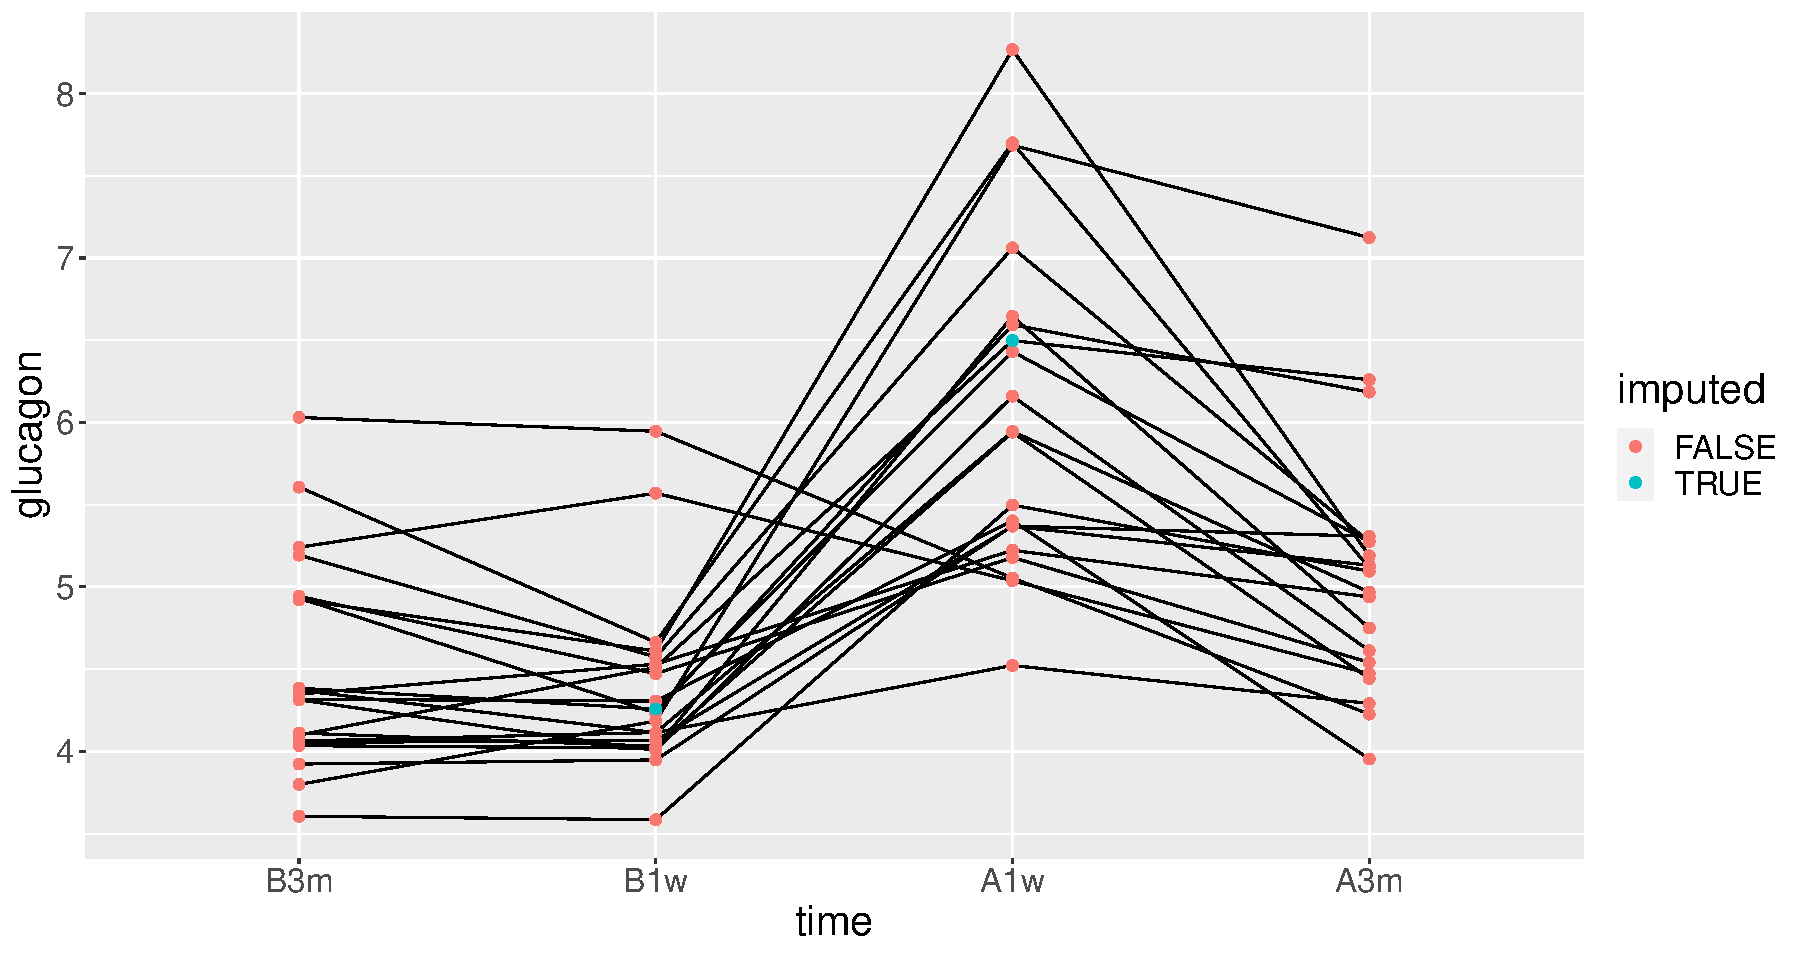
\includegraphics[trim={0 0 0 0},width=1\textwidth]{./figures/imputation.pdf}
\end{center}

It is possible to sample from the estimated distribution of the
missing value instead of using the most likely value, e.g. accounting
for residual variance and uncertainty related to parameter estimation:
\lstset{language=r,label= ,caption= ,captionpos=b,numbers=none}
\begin{lstlisting}
set.seed(10)
fitted(eUN.lmmNA, impute = TRUE, se = "total")
fitted(eUN.lmmNA, impute = TRUE, se = "total")
fitted(eUN.lmmNA, impute = TRUE, se = "total")
\end{lstlisting}

\begin{verbatim}
[1] 4.262434 6.305287
[1] 3.858267 5.871642
[1] 4.342624 6.905246
\end{verbatim}


\clearpage

\subsection{Multiple imputation}
\label{sec:orgfb2655f}

The \texttt{mlmm} function can used to perform stratify analyses, typically
useful when performing multiple imputations. Consider the wide format
of the dataset where a few values are missing:
\lstset{language=r,label= ,caption= ,captionpos=b,numbers=none}
\begin{lstlisting}
data(gastricbypassW, package = "LMMstar")
colSums(is.na(gastricbypassW))
\end{lstlisting}

\begin{verbatim}
          id      weight1      weight2      weight3      weight4 glucagonAUC1 glucagonAUC2 
           0            0            0            0            0            0            1 
glucagonAUC3 glucagonAUC4 
           1            0
\end{verbatim}


We use \texttt{mice} to generate a number of imputed datasets (here 5):
\lstset{language=r,label= ,caption= ,captionpos=b,numbers=none}
\begin{lstlisting}
library(mice)
set.seed(10)
gastricbypassW.mice <- mice(gastricbypassW, m = 5, printFlag = FALSE)
gastricbypassW.NNA <- complete(gastricbypassW.mice, action = "long")
table(gastricbypassW.NNA$.imp)
\end{lstlisting}

\begin{verbatim}
Advarselsbesked:
Number of logged events: 110

 1  2  3  4  5 
20 20 20 20 20
\end{verbatim}


We can then use \texttt{mlmm} to perform a separate linear regression per dataset:
\lstset{language=r,label= ,caption= ,captionpos=b,numbers=none}
\begin{lstlisting}
e.mlmm <- mlmm(glucagonAUC3~glucagonAUC2+weight2, data=gastricbypassW.NNA,
               by = ".imp", effects = "weight2=0", trace = FALSE)
model.tables(e.mlmm)
\end{lstlisting}

\begin{verbatim}
  by parameter  estimate       se      df     lower     upper     p.value
1  1   weight2 -204.6291 62.88617 17.0034 -337.3053 -71.95289 0.004670840
2  2   weight2 -194.4004 62.31006 17.0034 -325.8611 -62.93968 0.006231893
3  3   weight2 -211.9042 65.51654 17.0034 -350.1299 -73.67848 0.004872354
4  4   weight2 -199.8417 62.12071 17.0034 -330.9029 -68.78041 0.005058119
5  5   weight2 -199.9269 62.16057 17.0034 -331.0722 -68.78152 0.005065662
\end{verbatim}


and pool the results using Rubin's rule:
\lstset{language=r,label= ,caption= ,captionpos=b,numbers=none}
\begin{lstlisting}
model.tables(e.mlmm, method = "pool.rubin")
\end{lstlisting}

\begin{verbatim}
        estimate      se       df     lower     upper     p.value
<1, 5> -202.1404 63.4192 15.09811 -337.2388 -67.04208 0.006078676
\end{verbatim}


This matches\footnote{almost exactly, only the degrees of freedom are a
little different} the results obtained with the mice package:
\lstset{language=r,label= ,caption= ,captionpos=b,numbers=none}
\begin{lstlisting}
e.mice <- with(data=gastricbypassW.mice,exp=lm(glucagonAUC3~glucagonAUC2+weight2))
summary(pool(e.mice))
\end{lstlisting}

\begin{verbatim}
          term      estimate    std.error  statistic       df      p.value
1  (Intercept)  4.119699e+04 7674.2675772  5.3681988 15.08457 7.675819e-05
2 glucagonAUC2  7.038742e-02    0.3689445  0.1907805 15.23549 8.512165e-01
3      weight2 -2.021404e+02   63.4191998 -3.1873698 15.09481 6.080058e-03
\end{verbatim}


\clearpage

One can use the \texttt{plot} function to obtain a forest plot of the
individual estimates along with the pooled estimate:
\lstset{language=r,label= ,caption= ,captionpos=b,numbers=none}
\begin{lstlisting}
plot(e.mlmm, method = c("pool.rubin","none"))
\end{lstlisting}

\begin{center}
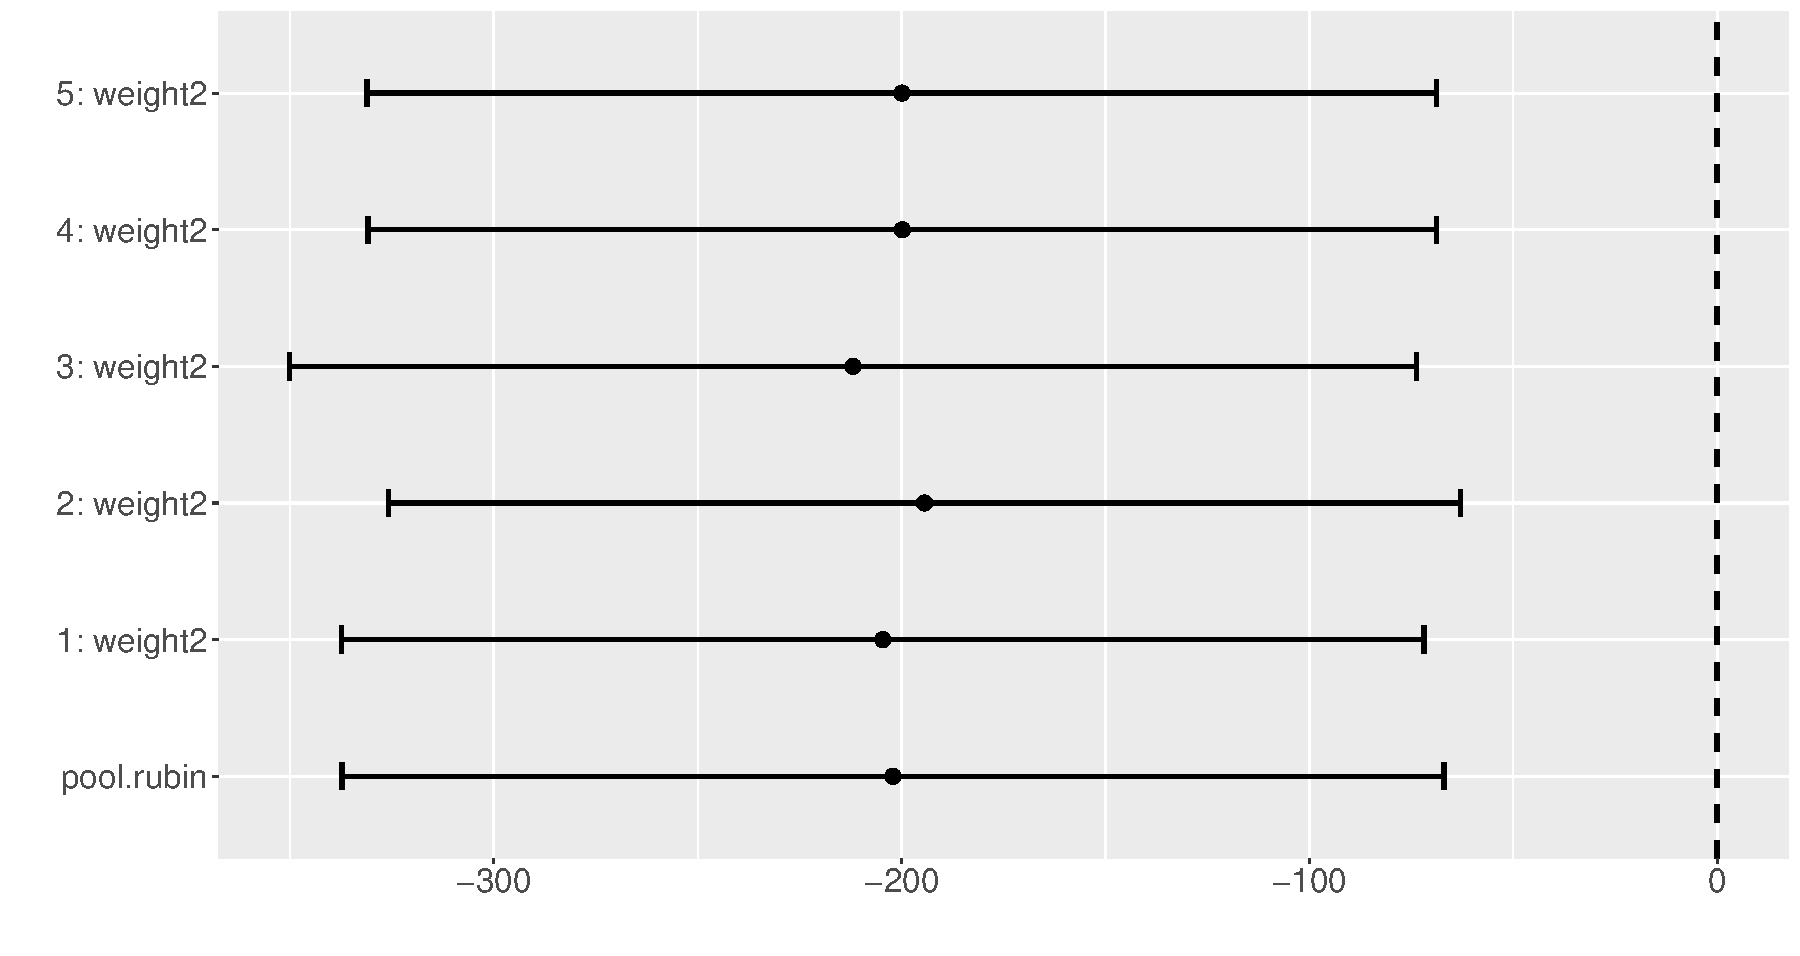
\includegraphics[trim={0 0 0 0},width=1\textwidth]{./figures/forestplot.pdf}
\end{center}

\clearpage

\section{Data generation}
\label{sec:org2042a10}
Simulate some data in the wide format:
\lstset{language=r,label= ,caption= ,captionpos=b,numbers=none}
\begin{lstlisting}
set.seed(10) ## ensure reproductibility
n.obs <- 100
n.times <- 4
mu <- rep(0,4)
gamma <- matrix(0, nrow = n.times, ncol = 10) ## add interaction
gamma[,6] <- c(0,1,1.5,1.5)
dW <- sampleRem(n.obs, n.times = n.times, mu = mu, gamma = gamma, format = "wide")
head(round(dW,3))
\end{lstlisting}

\begin{verbatim}
  id X1 X2 X3 X4 X5     X6     X7     X8    X9    X10     Y1     Y2     Y3     Y4
1  1  1  0  1  1  0 -0.367  1.534 -1.894 1.729  0.959  1.791  2.429  3.958  2.991
2  2  1  0  1  2  0 -0.410  2.065  1.766 0.761 -0.563  2.500  4.272  3.002  2.019
3  3  0  0  2  1  0 -1.720 -0.178  2.357 1.966  1.215 -3.208 -5.908 -4.277 -5.154
4  4  0  0  0  1  0  0.923 -2.089  0.233 1.307 -0.906 -2.062  0.397  1.757 -1.380
5  5  0  0  2  1  0  0.987  5.880  0.385 0.028  0.820  7.963  7.870  7.388  8.609
6  6  0  0  1  1  2 -1.075  0.479  2.202 0.900 -0.739  0.109 -1.602 -1.496 -1.841
\end{verbatim}


Simulate some data in the long format:
\lstset{language=r,label= ,caption= ,captionpos=b,numbers=none}
\begin{lstlisting}
set.seed(10) ## ensure reproductibility
dL <- sampleRem(n.obs, n.times = n.times, mu = mu, gamma = gamma, format = "long")
head(dL)
\end{lstlisting}

\begin{verbatim}
  id visit        Y X1 X2 X3 X4 X5         X6       X7        X8        X9        X10
1  1     1 1.791444  1  0  1  1  0 -0.3665251 1.533815 -1.894425 1.7288665  0.9592499
2  1     2 2.428570  1  0  1  1  0 -0.3665251 1.533815 -1.894425 1.7288665  0.9592499
3  1     3 3.958350  1  0  1  1  0 -0.3665251 1.533815 -1.894425 1.7288665  0.9592499
4  1     4 2.991198  1  0  1  1  0 -0.3665251 1.533815 -1.894425 1.7288665  0.9592499
5  2     1 2.500179  1  0  1  2  0 -0.4097541 2.065413  1.765841 0.7613348 -0.5630173
6  2     2 4.272357  1  0  1  2  0 -0.4097541 2.065413  1.765841 0.7613348 -0.5630173
\end{verbatim}


\clearpage

\section{Modifying default options}
\label{sec:orgc3a136b}
The \texttt{LMMstar.options} method enable to get and set the default options
used by the package. For instance, the default option for the information matrix is:
\lstset{language=r,label= ,caption= ,captionpos=b,numbers=none}
\begin{lstlisting}
LMMstar.options("type.information")
\end{lstlisting}

\begin{verbatim}
$type.information
[1] "observed"
\end{verbatim}


To change the default option to "expected" (faster to compute but less accurate p-values and confidence intervals in small samples) use:
\lstset{language=r,label= ,caption= ,captionpos=b,numbers=none}
\begin{lstlisting}
LMMstar.options(type.information = "expected")
\end{lstlisting}

To restore the original default options do:
\lstset{language=r,label= ,caption= ,captionpos=b,numbers=none}
\begin{lstlisting}
LMMstar.options(reinitialise = TRUE)
\end{lstlisting}

\clearpage

\section{R session}
\label{sec:orgb555587}
Details of the R session used to generate this document:
\lstset{language=r,label= ,caption= ,captionpos=b,numbers=none}
\begin{lstlisting}
sessionInfo()
\end{lstlisting}

\begin{verbatim}
R version 4.2.0 (2022-04-22 ucrt)
Platform: x86_64-w64-mingw32/x64 (64-bit)
Running under: Windows 10 x64 (build 19045)

Matrix products: default

locale:
[1] LC_COLLATE=Danish_Denmark.utf8  LC_CTYPE=Danish_Denmark.utf8    LC_MONETARY=Danish_Denmark.utf8
[4] LC_NUMERIC=C                    LC_TIME=Danish_Denmark.utf8    

attached base packages:
[1] stats     graphics  grDevices utils     datasets  methods   base     

other attached packages:
 [1] mice_3.14.0         lme4_1.1-29         Matrix_1.5-1        LMMstar_0.8.10     
 [5] nlme_3.1-158        ggpubr_0.4.0        multcomp_1.4-20     TH.data_1.1-1      
 [9] MASS_7.3-57         survival_3.3-1      mvtnorm_1.1-3       qqtest_1.2.0       
[13] emmeans_1.8.1-90002 ggplot2_3.4.0      

loaded via a namespace (and not attached):
 [1] tidyr_1.2.0         splines_4.2.0       carData_3.0-5       datawizard_0.6.1   
 [5] assertthat_0.2.1    stats4_4.2.0        bayestestR_0.13.0   globals_0.16.1     
 [9] numDeriv_2016.8-1.1 pillar_1.8.1        backports_1.4.1     lattice_0.20-45    
[13] glue_1.6.2          digest_0.6.29       ggsignif_0.6.3      minqa_1.2.4        
[17] colorspace_2.0-3    sandwich_3.0-2      cowplot_1.1.1       plyr_1.8.7         
[21] pcaPP_2.0-2         pkgconfig_2.0.3     broom_0.8.0         listenv_0.8.0      
[25] purrr_0.3.4         xtable_1.8-4        scales_1.2.1        copula_1.1-0       
[29] lava_1.6.10         tibble_3.1.8        ADGofTest_0.3       mgcv_1.8-40        
[33] generics_0.1.2      farver_2.1.1        car_3.1-0           withr_2.5.0        
[37] cli_3.4.1           effectsize_0.7.0.5  magrittr_2.0.3      estimability_1.4.1 
[41] future_1.28.0       fansi_1.0.3         parallelly_1.32.1   gsl_2.1-7.1        
[45] rstatix_0.7.0       textshaping_0.3.6   tools_4.2.0         lifecycle_1.0.3    
[49] pspline_1.0-19      stringr_1.4.0       munsell_0.5.0       stabledist_0.7-1   
[53] compiler_4.2.0      systemfonts_1.0.4   rlang_1.0.6         grid_4.2.0         
[57] nloptr_2.0.3        parameters_0.18.2   labeling_0.4.2      boot_1.3-28        
[61] lmerTest_3.1-3      gtable_0.3.1        codetools_0.2-18    abind_1.4-5        
[65] DBI_1.1.3           reshape2_1.4.4      R6_2.5.1            zoo_1.8-11         
[69] dplyr_1.0.9         future.apply_1.9.1  utf8_1.2.2          insight_0.18.4     
[73] ragg_1.2.2          stringi_1.7.6       parallel_4.2.0      Rcpp_1.0.8.3       
[77] vctrs_0.5.1         tidyselect_1.1.2    coda_0.19-4
\end{verbatim}

\clearpage

\section*{References}
\label{sec:org0dcd3f1}
\begingroup
\renewcommand{\section}[2]{}

\bibliographystyle{apalike}
\bibliography{bibliography}

\endgroup

\clearpage

\appendix
\titleformat{\section}
{\normalfont\Large\bfseries}{Appendix~\thesection}{1em}{}

\renewcommand{\thefigure}{\Alph{figure}}
\renewcommand{\thetable}{\Alph{table}}
\renewcommand{\theequation}{\Alph{equation}}

\setcounter{figure}{0}    
\setcounter{table}{0}    
\setcounter{equation}{0}    

\section{Likelihood in a linear mixed model}
\label{SM:likelihood}
Denote by \(\VY\) a vector of \(m\) outcomes, \(\VX\) a vector of
\(p\) covariates, \(\mu(\Vparam,\VX)\) the modeled mean, and
\(\Omega(\Vparam,\VX)\) the modeled residual variance-covariance. We
consider \(n\) replicates (i.e. \(\VY_1,\ldots,\VY_n)\) and
\(VX_1,\ldots,\VX_n\)) along with a vector of weights
\(\omega=(w_1,\ldots,w_n)\), which are by default all equal to 1.

\subsection{Log-likelihood}
\label{sec:org19b3c6a}

The restricted log-likelihood in a linear mixed model can then be
written:
\begin{align}
\Likelihood(\Vparam|\VY,\VX) =& \textcolor{\darkred}{ \frac{p}{2} \log(2\pi)-\frac{1}{2} \log\left(\left|\sum_{i=1}^n w_i \VX_i \Omega_i^{-1}(\Vparam) \trans{\VX}_i\right|\right)} \notag \\
& + \sum_{i=1}^{n} w_i \left(\textcolor{\darkblue}{-\frac{m}{2} \log(2\pi) - \frac{1}{2} \log\left|\Omega_i(\Vparam)\right| - \frac{1}{2} (\VY_i-\mu(\Vparam,\VX_i)) \Omega_i(\Vparam)^{-1} \trans{(\VY_i-\mu(\Vparam,\VX_i))}} \right)  \label{eq:log-likelihood}
\end{align}

This is what the \texttt{logLik} method is computing for the REML
criteria. The red term is specific to the REML criteria and prevents
from computing individual contributions to the likelihood\footnote{The REML is the
likelihood of the observations divided by the prior on the estimated
mean parameters \(\VparamHat_{\mu} \sim \Gaus(\mu,\left(\VX
 \Omega^{-1}(\Vparam) \trans{\VX}\right)^{-1})\). This corresponds to
\(\frac{1}{\sqrt{2\pi}^p \left|\left(\sum_{i=1}^n \VX_i
 \Omega_i^{-1}(\Vparam) \trans{\VX}_i\right)^{-1}\right|}
 \exp\left(-(\VparamHat_{\mu}-\mu)\left(2\sum_{i=1}^n \VX_i
 \Omega_i^{-1}(\Vparam)
 \trans{\VX}_i\right)^{-1})\trans{(\VparamHat_{\mu}-\mu)}\right)\)
Since \(\mu\) will be estimated to be \(\Vparam_{\mu}\), the
exponential term equals 1 and thus does not contribute to the
log-likelihood. One divided by the other term gives \(\sqrt{2\pi}^p
 \left(\left|\sum_{i=1}^n \VX_i \Omega_i^{-1}(\Vparam)
 \trans{\VX}_i\right|\right)^{-1}\). The log of this term equals the red
term}. The blue term is what \texttt{logLik} outputs for the ML criteria
when setting the argument \texttt{indiv} to \texttt{TRUE}.

\bigskip

\subsection{Score}
\label{sec:orgcc15bda}

 Using that \(\partial \log(\det(X))=tr(X^{-1}\partial(X))\), the
score is obtained by derivating once the log-likelihood, i.e., for
\(\theta \in \Vparam\):
\begin{align*}
   \Score(\theta) =& \dpartial[\Likelihood(\Vparam|\VY,\VX)][\theta]
= \textcolor{\darkred}{ \frac{1}{2} tr \left( \left(\sum_{i=1}^n w_i \VX_i \Omega_i^{-1}(\Vparam) \trans{\VX}_i\right)^{-1} \left(\sum_{i=1}^n w_i \VX_i \Omega_i^{-1}(\Vparam) \dpartial[\Omega_i(\Vparam)][\theta] \Omega_i(\Vparam)^{-1} \trans{\VX}_i\right)  \right) } \\
&+ \sum_{i=1}^n w_i \left( \textcolor{\darkblue}{ -\frac{1}{2} tr\left(\Omega_i(\Vparam)^{-1} \dpartial[\Omega_i(\Vparam)][\theta]\right) + \dpartial[\mu(\Vparam,\VX_i)][\theta] \Omega_i(\Vparam)^{-1} \trans{(\VY_i-\mu(\Vparam,\VX_i))} } \right. \\
 & \qquad \qquad \left. \textcolor{\darkblue}{ + \frac{1}{2} (\VY_i-\mu(\Vparam,\VX_i)) \Omega_i(\Vparam)^{-1} \dpartial[\Omega_i(\Vparam)][\theta] \Omega_i(\Vparam)^{-1} \trans{(\VY_i-\mu(\Vparam,\VX_i))} } \right).
\end{align*}

This is what the \texttt{score} method is computing for the REML
criteria. The red term is specific to the REML criteria and prevents
from computing the score relative to each cluster. The blue term is
what \texttt{score} outputs for the ML criteria when setting the argument
\texttt{indiv} to \texttt{TRUE}.

\bigskip

\clearpage

\subsection{Hessian}
\label{sec:org8484436}

Derivating a second time the log-likelihood gives the hessian, \(\Hessian(\Vparam)\), with element\footnote{if one is relative to the mean and the other to the variance then they are respectively \(\theta\) and \(\theta'\)}:
\begin{align*}
& \Hessian(\theta,\theta^{\prime}) = \ddpartial[\Likelihood(\Vparam|\VY,\VX)][\theta][\theta^{\prime}] = \dpartial[\Score(\theta)][\theta^{\prime}] \\
=& \textcolor{\darkred}{\frac{1}{2} tr \left( \left(\sum_{i=1}^n w_i \VX_i \Omega_i^{-1}(\Vparam) \trans{\VX}_i\right)^{-1} \left\{ \sum_{i=1}^n w_i \VX_i \Omega_i^{-1}(\Vparam) \left(\ddpartial[\Omega_i(\Vparam)][\theta][\theta^{\prime}] - 2 \dpartial[\Omega_i(\Vparam)][\theta] \Omega_i^{-1}(\Vparam) \dpartial[\Omega_i(\Vparam)][\theta^{\prime}]\right)\Omega_i(\Vparam)^{-1} \trans{\VX}_i \right.  \right.}  \\
& \textcolor{\darkred}{ \left. \left. + \left(\sum_{i=1}^n w_i \VX_i \Omega_i^{-1}(\Vparam) \dpartial[\Omega_i(\Vparam)][\theta] \Omega_i(\Vparam)^{-1} \trans{\VX}_i\right) \left(\sum_{i=1}^n w_i \VX_i\Omega_i^{-1}(\Vparam) \trans{\VX}_i \right)^{-1} \left(\sum_{i=1}^n w_i \VX_i \Omega_i^{-1}(\Vparam) \dpartial[\Omega_i(\Vparam)][\theta^{\prime}] \Omega_i(\Vparam)^{-1} \trans{\VX}_i\right) \right\} \right) } \\
& +\sum_{i=1}^n w_i \left( \textcolor{\darkblue}{ \frac{1}{2} tr\left(\Omega_i(\Vparam)^{-1} \dpartial[\Omega_i(\Vparam)][\theta^{\prime}] \Omega_i(\Vparam)^{-1} \dpartial[\Omega_i(\Vparam)][\theta] - \Omega_i(\Vparam)^{-1} \ddpartial[\Omega_i(\Vparam)][\theta][\theta^{\prime}] \right) } \right.\\
& \qquad \textcolor{\darkblue}{ -  \dpartial[\mu(\Vparam,\VX_i)][\theta] \Omega_i(\Vparam)^{-1} \dpartial[\Omega_i(\Vparam)][\theta^{\prime}] \Omega_i(\Vparam)^{-1} \trans{\Vvarepsilon_i(\Vparam)} - \dpartial[\mu(\Vparam,\VX_i)][\theta] \Omega_i(\Vparam)^{-1} \trans{\dpartial[\mu(\Vparam,\VX_i)][\theta^{\prime}]} } \\
& \qquad \left. \textcolor{\darkblue}{ + \frac{1}{2} \Vvarepsilon_i(\Vparam) \Omega_i(\Vparam)^{-1} \left(\ddpartial[\Omega_i(\Vparam)][\theta][\theta^{\prime}] - \dpartial[\Omega_i(\Vparam)][\theta^{\prime}] \Omega_i(\Vparam)^{-1} \dpartial[\Omega_i(\Vparam)][\theta] - \dpartial[\Omega_i(\Vparam)][\theta] \Omega_i(\Vparam)^{-1} \dpartial[\Omega_i(\Vparam)][\theta^{\prime}] \right) \Omega_i(\Vparam)^{-1} \trans{\Vvarepsilon_i(\Vparam)} } \right).
\end{align*}
where \(\Vvarepsilon_i(\Vparam) = \VY_i-\mu(\Vparam,\VX_i)\).

\bigskip

The \texttt{information} method will (by default) return the (observed)
information which is the opposite of the hessian. So multiplying the
previous formula by -1 gives what \texttt{information} output for the REML
criteria. The red term is specific to the REML criteria and prevents
from computing the information relative to each cluster. The blue term
is what \texttt{information} outputs for the ML criteria (up to a factor -1)
when setting the argument \texttt{indiv} to \texttt{TRUE}.

\bigskip

A possible simplification is to use the expected hessian at the maximum likelihood. Indeed for
any deterministic matrix \(A\):
\begin{itemize}
\item \(\Esp[A \trans{(\VY_i-\mu(\Vparam,\VX_i))}|\VX_i] = 0\)
\item \(\Esp[(\VY_i-\mu(\Vparam,\VX_i)) A \trans{(\VY_i-\mu(\Vparam,\VX_i))}||\VX_i] = tr(A \Var(\VY_i-\mu(\Vparam,\VX_i)))\)
\end{itemize}
when \(\Esp[\VY_i-\mu(\Vparam,\VX_i)]=0\). This leads to:
\begin{align}
 & \Esp[\Hessian(\theta,\theta^{\prime})|\VX] \notag\\ 
 &= \textcolor{\darkred}{ \frac{1}{2} tr \left( \left(\sum_{i=1}^n w_i \VX_i \Omega_i^{-1}(\Vparam) \trans{\VX}_i\right)^{-1}  \left\{ \sum_{i=1}^n w_i \VX_i \Omega_i^{-1}(\Vparam) \left( \ddpartial[\Omega_i(\Vparam)][\theta][\theta^{\prime}] - 2 \dpartial[\Omega_i(\Vparam)][\theta]  \Omega_i^{-1}(\Vparam) \dpartial[\Omega_i(\Vparam)][\theta^{\prime}]\right) \Omega_i(\Vparam)^{-1} \trans{\VX}_i \right.  \right.} \notag \\
 & \textcolor{\darkred}{ \left. \left. +  \left(\sum_{i=1}^n w_i \VX_i \Omega_i^{-1}(\Vparam) \dpartial[\Omega_i(\Vparam)][\theta] \Omega_i(\Vparam)^{-1} \trans{\VX}_i\right) \left(\sum_{i=1}^n w_i \VX_i \Omega_i^{-1}(\Vparam) \trans{\VX}_i \right)^{-1} \left(\sum_{i=1}^n w_i \VX_i \Omega_i^{-1}(\Vparam) \dpartial[\Omega_i(\Vparam)][\theta^{\prime}] \Omega_i(\Vparam)^{-1} \trans{\VX}_i\right) \right\} \right) } \notag\\
 & + \sum_{i=1}^n w_i \left( \textcolor{\darkblue}{
- \frac{1}{2} tr\left(\Omega_i(\Vparam)^{-1} \dpartial[\Omega_i(\Vparam)][\theta^{\prime}] \Omega_i(\Vparam)^{-1} \dpartial[\Omega_i(\Vparam)][\theta]\right)
 - \dpartial[\mu(\Vparam,\VX_i)][\theta] \Omega_i(\Vparam)^{-1} \trans{\dpartial[\mu(\Vparam,\VX_i)][\theta^{\prime}]}
 } \right) \label{eq:expectedInfo}
\end{align}

This is what \texttt{information} output when the argument \texttt{type.information}
is set to \texttt{"expected"} (up to a factor -1).

\clearpage

\subsection{Degrees of freedom}
\label{sec:org9cafd88}

Degrees of freedom are computed using a Satterthwaite approximation,
i.e. for an estimate coefficient \(\widehat{\beta}\in\widehat{\Vparam}\) with standard
error \(\sigma_{\widehat{\beta}}\), the degree of freedom is:
\begin{align*}
df\left(\sigma_{\widehat{\beta}}\right) = \frac{2 \sigma^4_{\widehat{\beta}}}{\Var[\widehat{\sigma}_{\widehat{\beta}}]}
\end{align*}
Using a first order Taylor expansion we can approximate the variance term as:
\begin{align*}
\Var[\widehat{\sigma}_{\widehat{\beta}}] & \approx \dpartial[\widehat{\sigma}_{\widehat{\beta}}][\Vparam] \Sigma_{\Vparam}  \trans{\dpartial[\widehat{\sigma}_{\widehat{\beta}}][\Vparam]} \\
& \approx c_{\beta} \left(\widehat{\Information}_{\widehat{\Vparam}}\right)^{-1} \dpartial[\widehat{\Information}_{\widehat{\Vparam}}][\Vparam] \left(\widehat{\Information}_{\widehat{\Vparam}}\right)^{-1} \trans{c_{\beta}} \Sigma_{\Vparam} \trans{c_{\beta}} \left(\widehat{\Information}_{\widehat{\Vparam}}\right)^{-1} \trans{\dpartial[\widehat{\Information}_{\widehat{\Vparam}}][\Vparam]} \left(\widehat{\Information}_{\widehat{\Vparam}}\right)^{-1} c_{\beta}
\end{align*}

where \(\Sigma_{\Vparam}\) is the variance-covariance matrix of all
  model coefficients, \(\Information_{\Vparam}\) the information
  matrix for all model coefficients, \(c_{\beta}\) a matrix used to
  select the element relative to \(\beta\) in the first derivative of
  the information matrix, and \(\dpartial[.][\Vparam]\) denotes the
  vector of derivatives with respect to all model coefficients.

\bigskip

The derivative of the information matrix (i.e. negative hessian) can
then be computed using numerical derivatives or using analytical
formula. To obtain the later we first notice that:
\begin{align}
&\Hessian(\theta,\theta^{\prime}) = \Esp[\Hessian(\theta,\theta^{\prime})|\VX] \notag \\
& + \sum_{i=1}^n  w_i \left( \textcolor{\darkblue}{ tr\left(\Omega_i(\Vparam)^{-1} \dpartial[\Omega_i(\Vparam)][\theta^{\prime}] \Omega_i(\Vparam)^{-1} \dpartial[\Omega_i(\Vparam)][\theta] - \Omega_i(\Vparam)^{-1} \ddpartial[\Omega_i(\Vparam)][\theta][\theta^{\prime}] \right) } \right. \notag \\
& \qquad \textcolor{\darkblue}{ -  \dpartial[\mu(\Vparam,\VX_i)][\theta] \Omega_i(\Vparam)^{-1} \dpartial[\Omega_i(\Vparam)][\theta^{\prime}] \Omega_i(\Vparam)^{-1} \trans{\Vvarepsilon_i(\Vparam)}} \notag \\
& \qquad \left. \textcolor{\darkblue}{ + \frac{1}{2} \Vvarepsilon_i(\Vparam) \Omega_i(\Vparam)^{-1} \left(\ddpartial[\Omega_i(\Vparam)][\theta][\theta^{\prime}] - \dpartial[\Omega_i(\Vparam)][\theta^{\prime}] \Omega_i(\Vparam)^{-1} \dpartial[\Omega_i(\Vparam)][\theta] - \dpartial[\Omega_i(\Vparam)][\theta] \Omega_i(\Vparam)^{-1} \dpartial[\Omega_i(\Vparam)][\theta^{\prime}] \right) \Omega_i(\Vparam)^{-1} \trans{\Vvarepsilon_i(\Vparam)} } \right) \label{eq:diffInfo}
\end{align}
where
\begin{align*}
\Esp[\Hessian(\theta,\theta^{\prime})|\VX] &=& \textcolor{\darkred}{
\frac{1}{2} tr \left(A(\Vparam)^{-1} \left(\sum_{i=1}^n w_i b_i(\Vparam) B_i(\Vparam) \trans{b}_i(\Vparam) + C(\Vparam)A(\Vparam)^{-1} \trans{C}(\Vparam) \right)\right)
}  + \sum_{i=1}^n w_i \textcolor{\darkblue}{E_i(\Vparam)} \\
\textcolor{\darkblue}{E_i(\Vparam)} &=& \textcolor{\darkblue}{\frac{1}{2} tr\left(\Omega_i(\Vparam)^{-1} \dpartial[\Omega_i(\Vparam)][\theta^{\prime}] \Omega_i(\Vparam)^{-1} \dpartial[\Omega_i(\Vparam)][\theta]\right)
                                        - \dpartial[\mu(\Vparam,\VX_i)][\theta] \Omega_i(\Vparam)^{-1} \trans{\dpartial[\mu(\Vparam,\VX_i)][\theta^{\prime}]}} \\
\textcolor{\darkred}{A(\Theta)} &=& \textcolor{\darkred}{\sum_{i=1}^n w_i \VX_i \Omega_i^{-1}(\Vparam) \trans{\VX}_i }\\
\textcolor{\darkred}{B(\Theta)} &=& \textcolor{\darkred}{\ddpartial[\Omega_i(\Vparam)][\theta][\theta^{\prime}] - 2 \dpartial[\Omega_i(\Vparam)][\theta]  \Omega_i^{-1}(\Vparam) \dpartial[\Omega_i(\Vparam)][\theta^{\prime}] }\\
\textcolor{\darkred}{b_i(\Theta)} &=& \textcolor{\darkred}{\VX_i \Omega_i^{-1} }\\
\textcolor{\darkred}{C(\Theta)} &=& \textcolor{\darkred}{\sum_{i=1}^n w_i \VX_i \Omega_i^{-1}(\Vparam) \dpartial[\Omega_i(\Vparam)][\theta] \Omega_i(\Vparam)^{-1} \trans{\VX}_i }
\end{align*}
So we will first derive the derivative of
\(\Esp[\Hessian(\theta,\theta^{\prime})|\VX]\) and then the one of the
blue term in \autoref{eq:diffInfo}.  To simplify the derivation of the
formula we will only derive them at the maximum likelihood, i.e. when
\(\Esp\left[\dpartial[\Hessian(\theta,\theta^{\prime}|\VX)][\theta^{\prime\prime}]\right]=\frac{\partial
\Esp[\Hessian(\theta,\theta^{\prime}|\VX)]}{\partial
\theta^{\prime\prime}}\) where the expectation is taken over
\(\VX\). We first notice that the derivative with respect to the mean
parameters is 0. So we just need to compute the derivative with
respect to a variance parameter \(\theta^{\prime\prime}\):
\begin{align*}
 & \frac{\partial \textcolor{\darkred}{ A(\Vparam)^{-1} \left(\sum_{i=1}^n w_i b_i(\Vparam) B_i(\Vparam) \trans{b}_i(\Vparam) + C(\Vparam)A(\Vparam)^{-1} \trans{C}(\Vparam) \right)}}{\partial \theta^{\prime\prime}} \\
 =& \textcolor{\darkred}{A(\Vparam)^{-1} \dpartial[A(\Vparam)][\theta^{\prime\prime}] A(\Vparam)^{-1} \left(\sum_{i=1}^n w_i b_i(\Vparam) B_i(\Vparam) \trans{b}_i(\Vparam) + C(\Vparam)A(\Vparam)^{-1} \trans{C}(\Vparam) \right)} \\
 & +\textcolor{\darkred}{A(\Vparam)^{-1} \left(\sum_{i=1}^n w_i \left(
 \dpartial[b_i(\Vparam)][\theta^{\prime\prime}]  B_i(\Vparam) \trans{b}_i(\Vparam)
 + b_i(\Vparam) \dpartial[B_i(\Vparam)][\theta^{\prime\prime}]   \trans{b}_i(\Vparam)
 + b_i(\Vparam) B_i(\Vparam) \dpartial[\trans{b}_i(\Vparam)][\theta^{\prime\prime}] \right. \right. } \\
& \qquad \qquad \qquad \qquad \quad + \textcolor{\darkred}{\left. \left.
 \dpartial[C(\Vparam)][\theta^{\prime\prime}]  A^{-1}(\Vparam) \trans{C}(\Vparam)
 + C(\Vparam) A^{-1}\dpartial[A(\Vparam)][\theta^{\prime\prime}]A^{-1}   \trans{C}(\Vparam)
 + C(\Vparam) A^{-1}(\Vparam) \dpartial[\trans{C}(\Vparam)][\theta^{\prime\prime}]
\right) \right)}
\end{align*}

and

\begin{align*}
 \dpartial[\textcolor{\darkblue}{E(\Vparam)}][\theta^{\prime\prime}]=&
 \sum_{i=1}^n w_i \left( \textcolor{\darkblue}{
- \frac{1}{2} tr\left(
-2\Omega_i(\Vparam)^{-1} \dpartial[\Omega_i(\Vparam)][\theta^{\prime\prime}] \Omega_i(\Vparam)^{-1} \dpartial[\Omega_i(\Vparam)][\theta^{\prime}] \Omega_i(\Vparam)^{-1} \dpartial[\Omega_i(\Vparam)][\theta] \right. } \right. \\
& \qquad \qquad \textcolor{\darkblue}{\left. + \Omega_i(\Vparam)^{-1} \ddpartial[\Omega_i(\Vparam)][\theta^{\prime}][\theta^{\prime\prime}] \Omega_i(\Vparam)^{-1} \dpartial[\Omega_i(\Vparam)][\theta]
+ \Omega_i(\Vparam)^{-1} \dpartial[\Omega_i(\Vparam)][\theta^{\prime}] \Omega_i(\Vparam)^{-1} \ddpartial[\Omega_i(\Vparam)][\theta][\theta^{\prime\prime}]
\right)} \\
& \qquad \qquad  \textcolor{\darkblue}{\left. + \dpartial[\mu(\Vparam,\VX_i)][\theta] \Omega_i(\Vparam)^{-1} \dpartial[\Omega_i(\Vparam)][\theta^{\prime\prime}] \Omega_i(\Vparam)^{-1}   \trans{\dpartial[\mu(\Vparam,\VX_i)][\theta^{\prime}]}
 \right)}
\end{align*}

where:
\begin{align*}
\textcolor{\darkred}{\dpartial[A(\Vparam)][\theta^{\prime\prime}]} &= \textcolor{\darkred}{\sum_{i=1}^n w_i \VX_i \Omega^{-1}_i(\Vparam) \dpartial[\Omega_i(\Vparam)][\theta^{\prime\prime}]\Omega^{-1}_i(\Vparam) \trans{\VX}_i} \\
\textcolor{\darkred}{\dpartial[b_i(\Vparam)][\theta^{\prime\prime}]} &= \textcolor{\darkred}{\VX_i \Omega^{-1}_i(\Vparam) \dpartial[\Omega_i(\Vparam)][\theta^{\prime\prime}]\Omega^{-1}_i(\Vparam)} \\
\textcolor{\darkred}{\dpartial[B_i(\Vparam)][\theta^{\prime\prime}]} &= \textcolor{\darkred}{
  \frac{\partial^3 \Omega_i(\Vparam)}{\theta\theta^{\prime}\theta^{\prime\prime}} } \\
  & \textcolor{\darkred}{ - 2 \left(
  \ddpartial[\Omega_i(\Vparam)][\theta][\theta^{\prime\prime}]\Omega^{-1}_i(\Vparam)\dpartial[\Omega_i(\Vparam)][\theta^{\prime}]
+ \dpartial[\Omega_i(\Vparam)][\theta]\Omega^{-1}_i(\Vparam)\dpartial[\Omega_i(\Vparam)][\theta^{\prime\prime}]\Omega^{-1}_i(\Vparam)\dpartial[\Omega_i(\Vparam)][\theta^{\prime}]
+ \dpartial[\Omega_i(\Vparam)][\theta]\Omega^{-1}_i(\Vparam)\ddpartial[\Omega_i(\Vparam)][\theta^{\prime}][\theta^{\prime\prime}]
\right)
  } \\
\textcolor{\darkred}{\dpartial[C(\Vparam)][\theta^{\prime\prime}]} &= \textcolor{\darkred}{\sum_{i=1}^n w_i \VX_i \Omega^{-1}_i(\Vparam) \left(
\dpartial[\Omega_i(\Vparam)][\theta^{\prime\prime}] \Omega^{-1}_i(\Vparam) \dpartial[\Omega_i(\Vparam)][\theta]
+ \ddpartial[\Omega_i(\Vparam)][\theta][\theta^{\prime\prime}]
+ \dpartial[\Omega_i(\Vparam)][\theta] \Omega^{-1}_i(\Vparam) \dpartial[\Omega_i(\Vparam)][\theta^{\prime\prime}]
\right) \Omega^{-1}_i(\Vparam) \trans{\VX}_i} 
\end{align*}



\clearpage

\section{Likelihood ratio test with the REML criterion}
\label{SM:LRT-REML}
The blue term of \autoref{eq:log-likelihood} in the log-likelihood is
invariant to re-parameterisation while the red term is not. This means
that a re-parametrisation of \(X\) into \(\tilde{X} = B X\) with \(B\)
invertible would not change the likelihood when using ML but would
decrease the log-likelihood by \(\log(|B|)\) when using REML. \newline
Let's take an example:
\lstset{language=r,label= ,caption= ,captionpos=b,numbers=none}
\begin{lstlisting}
## data(dfL, package = "LMMstar")
dfTest <- dfL
dfTest$glucagon2 <- dfTest$glucagon*2
\end{lstlisting}

where we multiply one column of the design matrix by 2. As mentionned
previously this does not affect the log-likelihood when using ML:
\lstset{language=r,label= ,caption= ,captionpos=b,numbers=none}
\begin{lstlisting}
eML.lmmUN <- lmm(weight ~ time+glucagon, data = dfTest, repetition = ~time|id, method = "ML")
eML.lmmUN2 <- lmm(weight ~ time+glucagon2, data = dfTest, repetition = ~time|id, method = "ML")
\end{lstlisting}

\lstset{language=r,label= ,caption= ,captionpos=b,numbers=none}
\begin{lstlisting}
logLik(eML.lmmUN)
logLik(eML.lmmUN2)
\end{lstlisting}

\begin{verbatim}
[1] -218.71
[1] -218.71
\end{verbatim}


but it does when using REML:
\lstset{language=r,label= ,caption= ,captionpos=b,numbers=none}
\begin{lstlisting}
eREML.lmmUN <- lmm(weight ~ time + glucagon, data = dfTest, repetition = ~time|id, method = "REML")
eREML.lmmUN2 <- lmm(weight ~ time + glucagon2, data = dfTest, repetition = ~time|id, method = "REML")
\end{lstlisting}

\lstset{language=r,label= ,caption= ,captionpos=b,numbers=none}
\begin{lstlisting}
logLik(eREML.lmmUN)-logLik(eREML.lmmUN2)
log(2)
\end{lstlisting}

\begin{verbatim}
[1] 0.6931472
[1] 0.6931472
\end{verbatim}


Therefore, when comparing models with different mean effects there is
a risk that the difference (or part of it) in log-likelihood is due to
a new parametrisation and no only to a difference in model fit. This
would typically be the case when adding an interaction where we can
have a smaller restricted log-likehood when considering a more complex
model:

\lstset{language=r,label= ,caption= ,captionpos=b,numbers=none}
\begin{lstlisting}
set.seed(5) 
dfTest$ff <- rbinom(NROW(dfTest), size = 1, prob = 0.5)
logLik(lmm(weight ~ time+glucagon, data = dfTest, repetition = ~time|id, method = "REML"))
logLik(lmm(weight ~ time+glucagon*ff, data = dfTest, repetition = ~time|id, method = "REML"))
\end{lstlisting}

\begin{verbatim}
[1] -216.3189
[1] -216.8425
\end{verbatim}


This is quite counter-intuitive as more complex model should lead to
better fit and would never happen when using ML:
\lstset{language=r,label= ,caption= ,captionpos=b,numbers=none}
\begin{lstlisting}
logLik(lmm(weight ~ time + glucagon, data = dfTest, repetition = ~time|id, method = "ML"))
logLik(lmm(weight ~ time + glucagon*ff, data = dfTest, repetition = ~time|id, method = "ML"))
\end{lstlisting}

\begin{verbatim}
[1] -218.71
[1] -218.6259
\end{verbatim}


This is why, unless one knows what he/she is doing, it is not
recommanded to use likelihood ratio test to assess relevance of mean
parameters in mixed models estimated with REML.

\clearpage

\section{Sum of squares in a linear mixed model}
\label{SM:sumSquares}
All mixed models implemented in LMMstar can be written as:
\[ Y_{it} = X_{it}\beta + \varepsilon_{it} \text{ where } \varepsilon_{i} \sim \Gaus\left(0,\Omega\right)\]
where \(Y\) denote the outcome repeteadly measured within each cluster
\(i\) where \(t\) indexes the repetitions. \(X\) denotes the
covariates, \(\beta\) the mean parameters, \(\varepsilon\) the
residuals, and \(\Omega\) the residual variance-covariance matrix.
\(\Omega\) must be positive definite so there must exist a square
postive definite matrix \(\Omega^{1/2}\) such that
\(\Omega^{1/2}\Omega^{1/2} = \Omega\). Therefore the previous model is
equivalent to:
\[ Y^*_{it} = X^*_{it}\beta + \varepsilon^*_{it} \text{ where } \varepsilon_{i} \sim \Gaus\left(0,I_T\right)\]
where \(Y^*_{i} = \Omega^{-1/2} Y_{i}\), \(X^*_{i} = \Omega^{-1/2}
X_{i}\), \(\varepsilon^*_{i} = \Omega^{-1/2} \varepsilon_{i}\), and
\(I_x\) is the identity matrix with \(x\) rows and columns. One can
then introduce the projectors \(H= X \left(\trans{X}\Omega^{-1}
X\right)^{-1}\trans{X} \Omega^{-1}\) and \(H^*= X^*
\left(\trans{X^*}X^*\right)^{-1}\trans{X^*}\) onto the space spanned
by \(X\) and \(X^*\) respectively. We can now define the "normalized"
residual sum of squares as the squared sum of the normalized
residuals:
\begin{align*}
SSE^* = \trans{\varepsilon^*} \varepsilon^* &= \trans{Y^*} (I_{nT}-H^*) Y^* \\
&= \trans{Y} \Omega^{-1} Y - \trans{Y} \Omega^{-1} X \left(\trans{X}\Omega^{-1} X\right)^{-1} \trans{X} \Omega^{-1} Y \\
&= \trans{Y} (I_{nT}-\trans{H}) \Omega^{-1} (I_{nT}-H) Y 
\end{align*}
The previous to last line uses that: \((I_{nT}-\trans{H}) \Omega^{-1}
(I_{nT}-H)= \Omega^{-1} - \trans{H} \Omega^{-1} - \Omega^{-1}H +
\trans{H} \Omega^{-1} H = \Omega^{-1} - \trans{H}\Omega^{-1}\) as
\(\trans{H} \Omega^{-1} H = \Omega^{-1}HH=\Omega^{-1}H\) since \(H\)
is a projector. Note that compared to the "traditional" SSE defined
for linear regression and random effect models (e.g. see
\cite{christensen2002plane} section 2.7), \(SSE=\delta SSE^{*}\) where
\(\delta\) is the residual variance conditional on any random effects,
i.e. \(SSE^{*}\) are the residual degrees of freedom. This is because
the same definition for the sum of squares is used except that
\(\varepsilon_{i} \sim \Gaus\left(0,\delta\Omega\right)\).

\bigskip

We can also define the "normalized" regression sum of squares:
\begin{align*}
SSR^* = \trans{(X^*\beta)}X^*\beta &= \trans{\left(H^* Y^*\right)} H^* Y^* = \trans{Y^*} H^* Y^* \\
&= \trans{Y} \trans{H} \Omega^{-1} Y^* = \trans{Y} \trans{H} \trans{H} \Omega^{-1} Y^* = \trans{Y} \trans{H} \Omega^{-1} H Y^* \\
&= \widehat{\beta} \trans{X} \Omega^{-1} X \widehat{\beta}
\end{align*}
where \(\widehat{\beta}= \left(\trans{X}\Omega^{-1}
X\right)^{-1}\trans{X} \Omega^{-1} Y\). Note that when using the
expected information \(SSR^* = \widehat{\beta}
\Sigma^{-1}_{\widehat{\beta}} \widehat{\beta}\), i.e. it is the
F-statistics times the number of parameters. Again the "traditional"
SSR defined for linear regression and random effect models is
proportional to this normalized SSR: \(SSR=\delta SSR^{*}\).

\bigskip

The proportion of explained variance of \(p\) parameters can thus be
re-expressed as:
\begin{align*}
R^2 &= \frac{SSR}{SSR+SSE} = \frac{SSR^*}{SSR^*+SSE^*}= \frac{Fp}{Fp+df}
\end{align*}

where \(df\) denotes the residual degrees of freedom, typically
\(n-p\) in a univariate linear model fitted with \(n\)
observations. \newline \Warning In practice \(df\) is estimated using the
Satterthwaite approximation of the degrees of freedom of the
regression coefficient. This is only equivalent to the "SSR/SSE"
formula in univariate linear regression.

\bigskip
\bigskip

\textbf{Illustration for a univariate linear model:}

\bigskip

Data without missing values:
\lstset{language=r,label= ,caption= ,captionpos=b,numbers=none}
\begin{lstlisting}
df.aov <- dfL[!is.na(dfL$glucagon),]
\end{lstlisting}

Traditional anova decomposition:
\lstset{language=r,label= ,caption= ,captionpos=b,numbers=none}
\begin{lstlisting}
e.lm <- lm(weight ~ time + glucagon, data = df.aov)
car::Anova(e.lm, type = "II")
\end{lstlisting}

\begin{verbatim}
Anova Table (Type II tests)

Response: weight
           Sum Sq Df F value    Pr(>F)    
time       6367.3  3  6.4308 0.0006329 ***
glucagon   1964.8  1  5.9531 0.0171207 *  
Residuals 24093.1 73                      
---
Signif. codes:  0 '***' 0.001 '**' 0.01 '*' 0.05 '.' 0.1 ' ' 1
\end{verbatim}


Fit \texttt{lmm}:
\lstset{language=r,label= ,caption= ,captionpos=b,numbers=none}
\begin{lstlisting}
e.lmm <- lmm(weight ~ time + glucagon, data = df.aov)
\end{lstlisting}

Residual sum of squares (SSE):
\lstset{language=r,label= ,caption= ,captionpos=b,numbers=none}
\begin{lstlisting}
SSEstar <- crossprod(residuals(e.lmm, type = "normalized"))
c(SSEstar = SSEstar, SSE = SSEstar * sigma(e.lmm))
\end{lstlisting}

\begin{verbatim}
SSEstar      SSE 
  73.00 24093.11
\end{verbatim}


The normalized SSE can also be obtained using the \texttt{df.residual} method:
\lstset{language=r,label= ,caption= ,captionpos=b,numbers=none}
\begin{lstlisting}
df.residual(e.lmm)
\end{lstlisting}

\begin{verbatim}
[1] 73
\end{verbatim}


Regression sum of squares (SSR):
\lstset{language=r,label= ,caption= ,captionpos=b,numbers=none}
\begin{lstlisting}
eBeta.lmm <- coef(e.lmm)
eVcov.lmm <- vcov(e.lmm, type.information = "expected")

SSRstar.glucagon <- eBeta.lmm[5] %*% solve(eVcov.lmm[5,5]) %*% eBeta.lmm[5] 
SSRstar.time <- eBeta.lmm[2:4] %*% solve(eVcov.lmm[2:4,2:4]) %*% eBeta.lmm[2:4] 
c(SSR.glucagon = SSRstar.glucagon * sigma(e.lmm),
  SSR.time = SSRstar.time * sigma(e.lmm),
  F.glucagon = SSRstar.glucagon,
  F.time = SSRstar.time/3)
\end{lstlisting}

\begin{verbatim}
SSR.glucagon     SSR.time   F.glucagon       F.time 
 1964.764452  6367.324429     5.953062     6.430810
\end{verbatim}


So the proportion of explained variance is:
\lstset{language=r,label= ,caption= ,captionpos=b,numbers=none}
\begin{lstlisting}
R2.glucagon <- SSRstar.glucagon/(SSRstar.glucagon+SSEstar)
R2.glucagon
\end{lstlisting}

\begin{verbatim}
           [,1]
[1,] 0.07540002
\end{verbatim}


and the corresponding partial correlation is:
\lstset{language=r,label= ,caption= ,captionpos=b,numbers=none}
\begin{lstlisting}
sign(coef(e.lmm)["glucagon"])*sqrt(R2.glucagon)
\end{lstlisting}

\begin{verbatim}
           [,1]
[1,] -0.2745906
\end{verbatim}


which matches the output of \texttt{partialCor}:
\lstset{language=r,label= ,caption= ,captionpos=b,numbers=none}
\begin{lstlisting}
summary(partialCor(e.lmm, R2 = TRUE))
\end{lstlisting}

\begin{verbatim}

		Partial correlation 

            estimate    se df  lower  upper  p.value
   timeB1w    -0.153 0.113 73 -0.378  0.072   0.1796
   timeA1w    -0.038 0.117 73  -0.27  0.195   0.7475
   timeA3m    -0.413 0.088 73 -0.589 -0.236 1.36e-05
   glucagon   -0.275 0.104 73 -0.482 -0.067   0.0102
   ------------------------------------------------ 
  Columns lower and upper contain 95% pointwise confidence intervals for each coefficient.
  Degrees of freedom were computed using a Satterthwaite approximation (column df). 

		Coefficient of determination (R2)

            estimate    se df  lower upper  p.value
   time        0.209 0.075 73  0.059 0.359 0.006976
   glucagon    0.075 0.057 73 -0.038 0.189 0.191156
   global      0.285 0.076 73  0.134 0.435 0.000328
   ------------------------------------------------ 
  Columns lower and upper contain 95% pointwise confidence intervals for each coefficient.
  Degrees of freedom were computed using a Satterthwaite approximation (column df).
\end{verbatim}

\clearpage

\section{Equivalent with other R packages}
\label{sec:org259eefc}

\subsection{nlme package}
\label{sec:orgbc42a95}

The model class obtained with the \texttt{lmm} function overlaps the model
class of the \texttt{lme} and \texttt{gls} functions from the nlme package.
\lstset{language=r,label= ,caption= ,captionpos=b,numbers=none}
\begin{lstlisting}
library(nlme)
\end{lstlisting}

For instance, the compound symmetry is equivalent to \texttt{corCompSymm}
correlation structure, or to a random intercept model (when the within
subject correlation is positive):
\lstset{language=r,label= ,caption= ,captionpos=b,numbers=none}
\begin{lstlisting}
eCS.gls <- gls(weight ~ time + glucagon, correlation = corCompSymm(form=~time|id),
               data = dfL, na.action = na.omit)
eCS.lme <- lme(weight ~ time + glucagon, random = ~1|id,
               data = dfL, na.action = na.omit)
logLik(eCS.lme)
logLik(eCS.gls)
logLik(eCS.lmm)
\end{lstlisting}

\begin{verbatim}
'log Lik.' -243.6005 (df=7)
'log Lik.' -243.6005 (df=7)
[1] -243.6005
\end{verbatim}


The estimated random effect also match:
\lstset{language=r,label= ,caption= ,captionpos=b,numbers=none}
\begin{lstlisting}
range(coef(eCS.lmm, effects = "ranef")-ranef(eCS.lme))
\end{lstlisting}

\begin{verbatim}
[1] -3.136988e-08  2.384361e-08
\end{verbatim}


Unstructured residual covariance matrix can also be obtained with
\texttt{gls}:
\lstset{language=r,label= ,caption= ,captionpos=b,numbers=none}
\begin{lstlisting}
eUN.gls <- gls(weight ~ time + glucagon,
               correlation = corSymm(form=~as.numeric(time)|id),
               weights = varIdent(form=~1|time),
               data = dfL, na.action = na.omit)
logLik(eUN.gls)
logLik(eUN.lmm)
\end{lstlisting}

\begin{verbatim}
'log Lik.' -216.3189 (df=15)
[1] -216.3189
\end{verbatim}


\clearpage

\subsection{lme4 package}
\label{sec:org8ea2484}

The model class obtained with the \texttt{lmm} function overlaps the model
class of the \texttt{lmer} function from the lme4 package.
\lstset{language=r,label= ,caption= ,captionpos=b,numbers=none}
\begin{lstlisting}
library(lme4)
library(lmerTest)
\end{lstlisting}

For instance, the compound symmetry is equivalent to a random
intercept model (when the within subject correlation is positive):
\lstset{language=r,label= ,caption= ,captionpos=b,numbers=none}
\begin{lstlisting}
eCS.lmer <- lmer(weight ~ time + glucagon + (1|id),
                 data = dfL)
logLik(eCS.lmer)
logLik(eCS.lmm)
\end{lstlisting}

\begin{verbatim}
'log Lik.' -243.6005 (df=7)
[1] -243.6005
\end{verbatim}


The estimated random effects match:
\lstset{language=r,label= ,caption= ,captionpos=b,numbers=none}
\begin{lstlisting}
range(coef(eCS.lmm, effects = "ranef")-ranef(eCS.lmer)$id)
\end{lstlisting}

\begin{verbatim}
[1] -3.167863e-08  2.406745e-08
\end{verbatim}


Nested random effects correspond to block unstructured:
\lstset{language=r,label= ,caption= ,captionpos=b,numbers=none}
\begin{lstlisting}
eBCS.lmer <- lmer(weight ~ time*group + (1|id/baseline),
                  data = dfL)
logLik(eBCS.lmer)
logLik(eBCS.lmm)
\end{lstlisting}

\begin{verbatim}
'log Lik.' -230.5328 (df=11)
[1] -230.5328
\end{verbatim}


And the estimated random effects still match:
\lstset{language=r,label= ,caption= ,captionpos=b,numbers=none}
\begin{lstlisting}
eRanefBCS.lmm <- coef(eBCS.lmm, effects = "ranef")
eRanefBCS.lmer <- ranef(eBCS.lmer)
## id
range(eRanefBCS.lmm[,"id"]-eRanefBCS.lmer$id)
## baseline
range(c(eRanefBCS.lmm[,"baseline1"],eRanefBCS.lmm[,"baseline2"])-ranef(eBCS.lmer)$`baseline:id`)
\end{lstlisting}

\begin{verbatim}
[1] -7.457484e-05  1.182242e-04
[1] -0.0001493705  0.0001080902
\end{verbatim}


\clearpage

An unstructure residual covariance matrix can also be obtained using
random slopes:
\lstset{language=r,label= ,caption= ,captionpos=b,numbers=none}
\begin{lstlisting}
eUN.lmer <- lmer(weight ~ time + glucagon + (0 + time|id),
                 data = dfL, control = lmerControl(check.nobs.vs.nRE = "ignore"))
logLik(eUN.lmer)
logLik(eUN.lmm)
\end{lstlisting}

\begin{verbatim}
'log Lik.' -216.3189 (df=16)
[1] -216.3189
\end{verbatim}


Note that however the uncertainty is quantified in a slightly different way, e.g.:
\lstset{language=r,label= ,caption= ,captionpos=b,numbers=none}
\begin{lstlisting}
anova(eUN.lmm)
\end{lstlisting}

\begin{verbatim}
	     Multivariate Wald test 

               F-statistic       df  p.value    
mean: time          86.743 (3,19.0) 2.84e-11 ***
    : glucagon      13.518 (1,13.7)  0.00257  **
\end{verbatim}


do not match
\lstset{language=r,label= ,caption= ,captionpos=b,numbers=none}
\begin{lstlisting}
anova(eUN.lmer)
\end{lstlisting}

\begin{verbatim}
Type III Analysis of Variance Table with Satterthwaite's method
          Sum Sq Mean Sq NumDF  DenDF F value    Pr(>F)    
time     114.275  38.092     3 20.483  87.242 7.784e-12 ***
glucagon  10.125  10.125     1 16.784  23.191 0.0001671 ***
---
Signif. codes:  0 '***' 0.001 '**' 0.01 '*' 0.05 '.' 0.1 ' ' 1
\end{verbatim}


I think this is because \texttt{lmer} base uncertainty computation on the
expected information (instead of the observed information). Doing so
leads to more similar results:
\lstset{language=r,label= ,caption= ,captionpos=b,numbers=none}
\begin{lstlisting}
eUN2.lmm <- lmm(weight ~ time + glucagon, repetition = ~time|id,
                structure = "UN", data = dfL, type.information = "expected")
suppressWarnings(anova(eUN2.lmm))
\end{lstlisting}

\begin{verbatim}
	     Multivariate Wald test 

               F-statistic       df  p.value    
mean: time          87.253 (3,22.5) 1.48e-12 ***
    : glucagon      23.198 (1,19.4) 0.000114 ***
\end{verbatim}


It is also possible to fit cross-random effects such as:
\lstset{language=r,label= ,caption= ,captionpos=b,numbers=none}
\begin{lstlisting}
data("Penicillin")
fm03 <- lmer(diameter ~ 1 + (1|plate) + (1|sample), Penicillin)
logLik(fm03)
\end{lstlisting}

\begin{verbatim}
'log Lik.' -165.4303 (df=4)
\end{verbatim}


using \texttt{lmm} with a small hack: using a block compound symmetry
structure with heterogeneous set to -1 to remove the correlation
coefficient for pairs that have none of the covariate defining the
blocks in common:
\lstset{language=r,label= ,caption= ,captionpos=b,numbers=none}
\begin{lstlisting}
Penicillin$index <- paste(Penicillin$sample,Penicillin$plate,sep=".")
Penicillin$id <- 1

e.lmm <- lmm(diameter ~ 1,
             repetition = ~index|id,
             structure = CS(list(~1,~plate+sample), heterogeneous = -1),
             data = Penicillin)
logLik(e.lmm)
\end{lstlisting}

\begin{verbatim}
[1] -165.4303
\end{verbatim}

\subsection{mmrm package}
\label{sec:org87dcfb1}

The package \texttt{mmrm} is an alternative implementation of mixed models
specified via covariance structures:
\lstset{language=r,label= ,caption= ,captionpos=b,numbers=none}
\begin{lstlisting}
library(mmrm)
e.mmrm <- mmrm(
  formula = FEV1 ~ RACE + SEX + ARMCD * AVISIT + us(AVISIT | USUBJID),
  data = fev_data
)
\end{lstlisting}

It leads nearly identical results compared to \texttt{lmm}:
\lstset{language=r,label= ,caption= ,captionpos=b,numbers=none}
\begin{lstlisting}
e.lmm <- lmm(
  formula = FEV1 ~ RACE + SEX + ARMCD * AVISIT,
  repetition = ~ AVISIT | USUBJID, structure = "UN",
  data = fev_data, type.information = "expected"
)
\end{lstlisting}
\lstset{language=r,label= ,caption= ,captionpos=b,numbers=none}
\begin{lstlisting}
logLik(e.mmrm) - logLik(e.lmm)
range(coef(e.mmrm) - coef(e.lmm))
range(vcov(e.mmrm) - vcov(e.lmm))
\end{lstlisting}

\begin{verbatim}
[1] -2.541298e-06
[1] -0.0001830095  0.0001626755
[1] -0.0003971008  0.0002047941
\end{verbatim}


The main differences are:
\begin{itemize}
\item \texttt{mmrm} uses the expected information matrix to quantify uncertainty
instead of the observed information matrix.
\item \texttt{mmrm} implements the Kenward and Roger method for computing the degrees of
freedom and not only the Satterthwaite approximation
\item \texttt{mmrm} implements different covariance patterns
\item \texttt{mmrm} is faster and probably more memorry efficient
\item \texttt{mmrm} have fewer post-processing methods (e.g. no \texttt{residuals}
function in the current CRAN version 0.2.2)
\end{itemize}

\subsection{effectsize package (\(R^2\) or \(\eta^2\))}
\label{sec:orgf50520b}

Partial \(\eta^2\) can be computed based on \texttt{lmer} using the effectsize package:
\lstset{language=r,label= ,caption= ,captionpos=b,numbers=none}
\begin{lstlisting}
library(effectsize)
eta_squared(eCS.lmer)
cat("\n")
\end{lstlisting}

\begin{verbatim}
# Effect Size for ANOVA (Type III)

Parameter | Eta2 (partial) |       95% CI
-----------------------------------------
time      |           0.92 | [0.89, 1.00]
glucagon  |           0.03 | [0.00, 1.00]

- One-sided CIs: upper bound fixed at [1.00].>
\end{verbatim}


and are approximately equal to what one can compute "manually":
\lstset{language=r,label= ,caption= ,captionpos=b,numbers=none}
\begin{lstlisting}
eCS.Wald <- anova(eCS.lmm)$multivariate
eCS.Wald$df.num*eCS.Wald$statistic/(eCS.Wald$df.num*eCS.Wald$statistic+eCS.Wald$df.denom)
\end{lstlisting}

\begin{verbatim}
[1] 0.92380363 0.03162017
\end{verbatim}


The will not be true for heteroschedastic models:
\lstset{language=r,label= ,caption= ,captionpos=b,numbers=none}
\begin{lstlisting}
eUN.Wald <- anova(eUN.lmm)$multivariate
eUN.Wald$df.num*eUN.Wald$statistic/(eUN.Wald$df.num*eUN.Wald$statistic+eUN.Wald$df.denom)
\end{lstlisting}

\begin{verbatim}
[1] 0.9319379 0.4965135
\end{verbatim}


compared to:
\lstset{language=r,label= ,caption= ,captionpos=b,numbers=none}
\begin{lstlisting}
eta_squared(eUN.lmer)
cat("\n")
\end{lstlisting}

\begin{verbatim}
# Effect Size for ANOVA (Type III)

Parameter | Eta2 (partial) |       95% CI
-----------------------------------------
time      |           0.93 | [0.87, 1.00]
glucagon  |           0.58 | [0.29, 1.00]

- One-sided CIs: upper bound fixed at [1.00].>
\end{verbatim}


But in that case both may be misleading as the proportion of explained
variance is not clearly defined.

\subsection{MuMIn package (\(R^2\))}
\label{sec:orgc264787}

\lstset{language=r,label= ,caption= ,captionpos=b,numbers=none}
\begin{lstlisting}
library(MuMIn)
r.squaredGLMM(eCS.lmer)
cat("\n")
\end{lstlisting}

\begin{verbatim}
           R2m       R2c
[1,] 0.2163302 0.9764382
\end{verbatim}


To reproduce these R2, we extract from the random intercept model:
\begin{itemize}
\item the residual variance
\end{itemize}
\lstset{language=r,label= ,caption= ,captionpos=b,numbers=none}
\begin{lstlisting}
sigmaW <- sigma(eCS.lmm)[1,1]-sigma(eCS.lmm)[1,2]
\end{lstlisting}

\begin{itemize}
\item the variance of the random effect
\end{itemize}
\lstset{language=r,label= ,caption= ,captionpos=b,numbers=none}
\begin{lstlisting}
sigmaB <- sigma(eCS.lmm)[1,2]
\end{lstlisting}

\begin{itemize}
\item the variance of the fitted values:
\end{itemize}
\lstset{language=r,label= ,caption= ,captionpos=b,numbers=none}
\begin{lstlisting}
sigma2_XB <- var(fitted(eCS.lmm))
\end{lstlisting}

and evalutae the ratios:
\lstset{language=r,label= ,caption= ,captionpos=b,numbers=none}
\begin{lstlisting}
c(R2m = sigma2_XB/(sigmaW + sigmaB + sigma2_XB),
  R2c = (sigma2_XB + sigmaB)/(sigmaW + sigmaB + sigma2_XB))
\end{lstlisting}

\begin{verbatim}
      R2m       R2c 
0.2163302 0.9764382
\end{verbatim}

\subsection{stats package (partial residuals)}
\label{sec:orgab45d96}

The function \texttt{residuals.lm} can be used to extract partial residuals
from \texttt{lm} objects:
\lstset{language=r,label= ,caption= ,captionpos=b,numbers=none}
\begin{lstlisting}
eIID.lm <- lm(weight ~ time + glucagon, data = dfL)
pRes.lm <- residuals(eIID.lm, type = "partial")
head(pRes.lm)
\end{lstlisting}

\begin{verbatim}
       time   glucagon
1  3.359543   1.475108
2 49.419060  39.475108
3 -8.145299 -16.024892
4 24.241798  20.475108
5 -8.407618 -12.624892
6 41.027985  33.075108
\end{verbatim}


Those generally differ (by a constant) from the one provided by
\texttt{residuals.lmm}:
\lstset{language=r,label= ,caption= ,captionpos=b,numbers=none}
\begin{lstlisting}
eIID.lmm <- lmm(weight ~ time + glucagon, data = dfL)
head(residuals(eIID.lmm, type = "partial", var = "glucagon"))
\end{lstlisting}

\begin{verbatim}
[1] -31.9349871   6.0650129 -49.4349871 -12.9349871 -46.0349871  -0.3349871
\end{verbatim}


Indeed, \texttt{residuals.lm} centers the design matrix of the variable
relative to which the partial residuals are computed:
\lstset{language=r,label= ,caption= ,captionpos=b,numbers=none}
\begin{lstlisting}
m.pres2 <- dfL$weight - cbind(model.matrix(~time,dfL), mean(dfL$glucagon)) %*% coef(eIID.lmm)
range(pRes.lm[,"glucagon"] - m.pres2, na.rm = TRUE)
\end{lstlisting}

\begin{verbatim}
[1] -3.348433e-13  4.654055e-13
\end{verbatim}


For continuous variable with a linear effect, these residuals can be
obtained by setting the \texttt{type} argument to \texttt{"partial-center"}:
\lstset{language=r,label= ,caption= ,captionpos=b,numbers=none}
\begin{lstlisting}
eIID.lmm <- lmm(weight ~ time + glucagon, data = dfL)
pRes.lmm <- residuals(eIID.lmm, type = "partial-center", var = "glucagon")
range(pRes.lm[,"glucagon"]-pRes.lmm)
\end{lstlisting}

\begin{verbatim}
[1] -3.330669e-13  4.725109e-13
\end{verbatim}


\Warning When evaluating the partial residuals relative to categorical
variables, interactions, or non-linear terms, the output obtained with
\texttt{partial-center} will not match the one of \texttt{residuals.lm}. Indeed
\texttt{partial-center} will, when numeric, center the original variable
whereas \texttt{residuals.lm} will center the column relative to the
coefficient in the design matrix.
\end{document}